% report_all_short.tex -- short summary of report_all.tex (Part III: data compared with SMASH, eta yields, X17 limit)
% Build: cd docs/latex && pdflatex report_all_short (three passes; no bibtex)
% Every number is taken from report_all.tex. Readability rewrite of 16 November 2026 (analyst's instructions I1-I4): results, their
% uncertainties, the evidence figures and their meaning; no internal labels in text, tables and captions; every caption states its
% selection in plain words and explains the symbols still printed inside the figure (\figlabels). Figures: plain-legend versions
% (*_plain*, trimmed ones as *_crop* copies without the hidden panels). Previous versions: scratchpad backups
% final/integ6/backup/short_all_writer/ (23:46), final/integ6/backup/allshort_writer_r/ (01:10), backup/allshort_final/ (02:57).
\documentclass[11pt,a4paper]{article}
\usepackage[T1]{fontenc}
\usepackage[utf8]{inputenc}
\usepackage{lmodern}
\usepackage[margin=2.0cm]{geometry}
\usepackage{amsmath}
\usepackage{graphicx}
\usepackage{booktabs}
\usepackage{tabularx}
\usepackage{longtable}
\usepackage{array}
\usepackage{xcolor}
\usepackage{caption}
\usepackage{float}
\usepackage{microtype}
\usepackage{xspace}
\usepackage[colorlinks=true,linkcolor=blue!50!black,urlcolor=blue!50!black]{hyperref}

\captionsetup{font=small,labelfont=bf,margin=0.3cm,singlelinecheck=false}
\setlength{\parskip}{0.4em}
\setlength{\parindent}{0pt}
\setlength{\emergencystretch}{3em}
\renewcommand{\arraystretch}{1.15}
\newcolumntype{L}{>{\raggedright\arraybackslash}X}

\newcommand{\pip}{\ensuremath{\pi^{+}}\xspace}
\newcommand{\pim}{\ensuremath{\pi^{-}}\xspace}
\newcommand{\piz}{\ensuremath{\pi^{0}}\xspace}
\newcommand{\ee}{\ensuremath{e^{+}e^{-}}\xspace}
\newcommand{\pipi}{\ensuremath{\pi^{+}\pi^{-}}\xspace}
\newcommand{\ppee}{\ensuremath{\pi^{+}\pi^{-}e^{+}e^{-}}\xspace}
\newcommand{\Mfour}{\ensuremath{M(\pi^{+}\pi^{-}e^{+}e^{-})}\xspace}
\newcommand{\Mee}{\ensuremath{M(e^{+}e^{-})}\xspace}
\newcommand{\Mpipi}{\ensuremath{M(\pi^{+}\pi^{-})}\xspace}
\newcommand{\nbinv}{\ensuremath{\mathrm{nb}^{-1}}\xspace}
\newcommand{\GeVcc}{\ensuremath{\mathrm{GeV}/c^{2}}\xspace}
\newcommand{\MeVcc}{\ensuremath{\mathrm{MeV}/c^{2}}\xspace}
\newcommand{\vz}{\ensuremath{v_z}\xspace}
\newcommand{\sigeta}{\ensuremath{\sigma(pp\to\eta X)}\xspace}
\newcommand{\BRX}{\ensuremath{\mathrm{BR}(\eta\to\pipi X17)\,\mathrm{BR}(X17\to\ee)}\xspace}
\newcommand{\keybox}[1]{\par\noindent\fcolorbox{blue!50!black}{blue!5}{\parbox{\dimexpr\linewidth-2\fboxsep-2\fboxrule\relax}{#1}}\par}
\newcommand{\inshort}[1]{\par\noindent\fcolorbox{blue!30}{blue!3}{\parbox{\dimexpr\linewidth-2\fboxsep-2\fboxrule\relax}{\textbf{In short:} #1}}\par}
% plain-words selections, written out in full in every caption (analyst's instruction I2)
\newcommand{\ptthree}{PT3 trigger (at least two sectors with an inner-TOF hit in coincidence with TOF or RPC, and at least three
inner-TOF paddles hit; trigger bit 8192)\xspace}
\newcommand{\selid}{pions and leptons identified by their START-free velocity (pions within 3$\sigma$, leptons within 5$\sigma$ of the
expected band; leptons with a matched RICH ring, pions without one); energy-loss-corrected momenta for all four tracks; all \ppee
combinations of each event whose four tracks pass the identification (an event can give more than one count)\xspace}
\newcommand{\selbase}{\ptthree; a reconstructed event vertex inside the target region ($\vz>-160$\,mm); \selid}
\newcommand{\selnovtx}{\ptthree; \selid}
\newcommand{\selnom}{\selbase; both pions used in the fit of the event vertex\xspace}
\newcommand{\cbsel}{CB $=2\sqrt{N_{++}N_{--}}$ from the like-sign data ($\pi^+\pi^-e^+e^+$, $\pi^+\pi^-e^-e^-$) with the same cuts, in
10\,\MeVcc cells of \Mfour}
\newcommand{\cbspread}{\cbsel, shared out over the \Mpipi slices and \Mee classes by the like-sign share of each 50\,\MeVcc band of \Mfour}
\newcommand{\smashsel}{SMASH p+p at 4.5\,GeV (standard, lepton and $\eta$ simulation sets, 221.05\,\nbinv each), every channel at its
SMASH cross section $\times$ PDG branching ratio $\times$ the $\eta$-decay physics weights, the same cuts (simulated trigger bit 8192),
simulated \Mfour$\times0.99615$ and \Mpipi$\times0.9952$ (moved to the data mass scale)\xspace}
\newcommand{\lumisel}{data counts $\times64/63$ (trigger-bit correction), $L=6079.2\,\nbinv$\xspace}
\newcommand{\seltyp}{the typical cuts of earlier analyses: angle between the \pipi and \ee momenta below $50^\circ$ in the laboratory and above
$140^\circ$ in the $\eta$ rest frame, \Mpipi below 0.46\,\GeVcc, \ee opening angle above $2^\circ$\xspace}
\newcommand{\slicesfive}{the five \Mpipi slices below 0.34, 0.34--0.37, 0.37--0.39, 0.39--0.43 and above 0.43\,\GeVcc}
\newcommand{\slicesfour}{the four \Mpipi slices 0.30--0.34, 0.34--0.37, 0.37--0.39 and 0.39--0.40\,\GeVcc}
\newcommand{\usel}{$0.30\le\Mpipi<0.40$\,\GeVcc and \Mee below 135\,\MeVcc (the \piz mass; above it $u$ is not defined); CB $=2\sqrt{N_{++}N_{--}}$
from the like-sign data with the same cuts, in 10\,\MeVcc cells of $u$, separately in \slicesfour}
\newcommand{\Sel}{\emph{Selection:}\xspace}
% explanation of the symbols that the figure itself still prints
\newcommand{\figlabels}[1]{{\footnotesize\emph{Symbols in the figure:} #1}}
% figure-heavy report: float pages must be well filled, and large floats may stand at the top of a text page (as in Part II)
\renewcommand{\topfraction}{0.9}\renewcommand{\bottomfraction}{0.6}\renewcommand{\textfraction}{0.07}\renewcommand{\floatpagefraction}{0.75}
\setcounter{topnumber}{3}\setcounter{bottomnumber}{2}\setcounter{totalnumber}{4}
\makeatletter
\newcommand{\floatbarrier}{\par\begingroup\let\@elt\relax\edef\@tempa{\@botlist\@deferlist\@dbldeferlist}\ifx\@tempa\@empty\else\clearpage\fi\endgroup}
\makeatother

\title{\Large $p + p \to \pi^{+}\pi^{-}e^{+}e^{-}$ Analysis Report\\[0.3em]
       \normalsize Short summary of Part III: the data compared with SMASH, the $\eta$ yields and the X17 limit}
\author{W.~Przygoda}
\date{16 November 2026}

\begin{document}
\maketitle
\vspace{-2.5em}

\keybox{\small\textbf{\large Key results in plain words}
\begin{enumerate}\setlength{\itemsep}{1pt}\setlength{\topsep}{2pt}
\item \textbf{$\eta$ production:} $\sigeta=0.43\pm0.17\,(\mathrm{measurement})\,^{+0.08}_{-0.03}\,(\mathrm{production~model})$\,mb, preliminary:
      $0.40\pm0.16$ of the SMASH $\eta$ (1.07\,mb); not presented as confirmed: below the published HADES values at 3.5\,GeV (1.14, 0.93\,mb),
      which SMASH matches. Largest open question: the make-up of the $\eta$ peak (direct decays alone 0.52\,mb, converted photons alone
      0.25\,mb; Fig.~\ref{fig:eta-summary}).
\item \textbf{The $\eta$ peak is measured:} $5088\pm432\,(\mathrm{stat})\pm584\,(\mathrm{syst})\pm245\,(\mathrm{MC})$ counts, 0.418 of SMASH; of
      the peak methods, the side bands are the only one that recovered the known answer on simulated pseudo-data (Fig.~\ref{fig:res-peaks}b).
\item \textbf{The $\eta$ bump is measured through its kinematic edge:} in the distance to the edge, $u$, one step of 21$\sigma$ at $u=0$,
      $0.426\pm0.020\,(\mathrm{stat})\pm0.034\,(\mathrm{syst})\pm0.030\,(\mathrm{MC})$ of the SMASH bump (simulated \piz Dalitz decay angle corrected
      to QED); \sigeta from the bump 0.444\,mb, as the peak (a weak test); a like-sign step is explained (pairs from the two \piz photons;
      consistent with the CB rule) (Figs.~\ref{fig:res-edgeus}, \ref{fig:res-edges}, \ref{fig:res-eesteps}); the background-subtracted bump
      area is not determined (Figs.~\ref{fig:res-peaks}a, \ref{fig:res-afters}).
\item \textbf{Full reconstruction of the bump with the ECAL photon} (feasibility): about 12\,\% of the bump as a clean peak; data/prediction
      $1.16\pm0.21$ or $0.84\pm0.15$ (simulated or data-like photon energy scale); needs the photon calibration, the module efficiency, a
      START-free photon cut, more simulation (Fig.~\ref{fig:res-ecals}).
\item \textbf{X17: no signal.} 90\,\% CL$_s$ limit: X17 makes at most 11\,\% of the direct decays ($r<0.114$), i.e.\ $\BRX<3.16\times10^{-5}$ at
      17\,\MeVcc (PDG 2026)\footnotemark{}; expected $2.7\times10^{-5}$; procedure fixed before the signal region was opened (Figs.~\ref{fig:x17-mee}, \ref{fig:x17-limit}).
\item \textbf{X17 against other searches:} two times weaker than BESIII at 17\,\MeVcc ($\approx1.5\times10^{-5}$); numerically similar
      to the HADES preliminary $2.58\times10^{-5}$, which is built differently, not a cross-check (Table~\ref{tab:x17other}).
\item \textbf{SMASH does not describe the spectrum shape} (data/SMASH 0.74--1.27 across \Mfour); 13--15\,\% of the data minus the combinatorial
      background in 0.40--0.70\,\GeVcc comes from the target walls, not simulated (Figs.~\ref{fig:res-befores}, \ref{fig:res-afters}, \ref{fig:res-wallss}).
\item \textbf{SMASH with a free scale per channel} (a description): the three $\eta$ signal channels share one scale, $0.46\pm0.06$ of SMASH
      ($0.57\pm0.07$ after correcting the downward bias that the noise of the simulated shapes causes, as measured on pseudo-data); the
      background above the peak is 10--30\,\% above SMASH; the model is incomplete ($p<0.001$) (Fig.~\ref{fig:res-freescale}).
\item \textbf{Checks that came out fine:} the requirement of a reconstructed event vertex keeps $99.4\pm2.1$\,\% of the $\eta$ (Fig.~\ref{fig:vtx}); the target walls
      carry only $3^{+4}_{-3}$\,\% of the $\eta$ signal (Fig.~\ref{fig:res-fetas}).
\item \textbf{A simulation defect:} HGeant decays the virtual photon of $\piz\to\gamma\ee$ isotropically, not as $1+\cos^2\theta^*$:
      simulated bump efficiency about 16\,\% too high; corrected in the bump edges (Fig.~\ref{fig:res-qed}).
\item \textbf{Typical cuts of earlier analyses (comparison only):} the data still exceed SMASH as it is by 16--45\,\% above the peak; no gain
      for the $\eta$ or for an X17 count (Fig.~\ref{fig:res-typcuts}). Drawn as in the earlier analysis, SMASH scaled to the data integral gets
      the total right but the parts wrong (bump about 20\,\% too high, above the peak about 10\,\% too low), and a three-scale fit gives $\eta$
      scales that move with the treatment of the simulated shapes (Figs.~\ref{fig:prev-m4}, \ref{fig:prev-fit}).
\end{enumerate}}
\footnotetext{\label{fn:x17pdg}With the PDG 2020 value $(2.68\pm0.11)\times10^{-4}$, which the fixed procedure used: $3.06\times10^{-5}$.}

\smallskip
The full report \texttt{report\_all.pdf} derives every number step by step; its Appendix~A, ``Decisions of the analyst'', lists the analysis
decisions behind these results.

%======================================================================
\section{Results}
\label{sec:res}
%======================================================================
Part~III compares the HADES p+p data at 4.5\,GeV (analysed alone in Part~II) with the SMASH simulation (Part~I), measures how many $\eta$
mesons the data contain and searches for a hypothetical light boson X17 in $\eta\to\pipi X17$, $X17\to\ee$. The combinatorial background (CB)
always comes from the like-sign data, never from the simulation.

\textbf{Conventions.} Unless a caption says otherwise, every number uses the \emph{nominal selection}: \selnom. The \emph{base selection}
(the base cuts of Part~II) is the same without the pion-vertex condition.

\emph{Trigger.} PT3, the main reaction trigger of the February 2022 beam time, requires fullSecMult\,$\ge2$ and iTOFPadMult\,$\ge3$: at least
two of the six sectors with a hit in the inner TOF wall (iTOF) together with a hit in the outer TOF wall or the RPC of the same sector, and at
least three inner-TOF paddles hit (P.~Tlusty, ``LVL1 trigger in Feb22 p+p 4.5\,GeV'', HADES internal presentation, 13 December 2024, with
the definition slide of I.~Ciepa\l{}). Only the bit of the trigger signal that arrives first is written: PT3 events carry bit 8192, while the
minimum-bias PT2 events (at least one such sector, recorded with a downscaling of 64) and the events that fired both PT2 and PT3 carry bit
4096. The events with bit 8192 therefore hold 63/64 of all PT3 events, and the data yields are multiplied by 64/63.

\emph{Event vertex.} Two vertex conditions are applied. First, the event must have a reconstructed event vertex: the vertex finder, the same
in data and simulation, takes the tracks that pass the beam axis within $-170<z<-30$\,mm and $r<20$\,mm and fits their common point if there
are at least two (otherwise the event carries $\vz=-1000$\,mm; the condition is written $\vz>-500$\,mm); the fitted point can lie outside
that window, as the vertex distributions of Figs.~\ref{fig:res-wallss} and \ref{fig:res-fetas} show. Second, the vertex must lie in the
target region, $\vz>-160$\,mm. The $\eta$ efficiency of the first condition is measured, $0.994\pm0.021$ (\S\ref{sec:phys}); the second acts
alike in data and simulation and is tested by moving its edge to $-150$ and $-170$\,mm (the selection term of Table~\ref{tab:syst}).

\emph{Normalisation and errors.} The CB is $2\sqrt{N_{++}N_{--}}$ of the like-sign counts with the same cuts; the simulation never provides
it. Data yields are counts $\times64/63$, $L=6079.2\,\nbinv$ ($\pm6.9$\,\%). SMASH enters with every channel at its own cross section
$\times$ PDG branching ratio $\times$ the $\eta$-decay physics weights, with its masses moved to the data mass scale. The $\eta$ scales
(data/SMASH) are quoted with the PDG 2020 branching ratios used in the simulation; \sigeta, BR$(\eta\to\ppee)$ and the X17 limit use PDG 2026
($2.76\times10^{-4}$ for $\eta\to\ppee$ instead of $2.68\times10^{-4}$). With PDG 2026 the scales are slightly lower (peak 0.409 instead of
0.418, bump edge in $u$ 0.424 instead of 0.426; double ratio peak/bump area 1.37 instead of 1.40); Fig.~\ref{fig:eta-summary}a and the X17
variants show them in that form. A \emph{count} is one stored \ppee combination; yields are not corrected for efficiency. Errors are statistical
(stat; from whole events), systematic (syst), simulation statistics (MC) and normalisation (norm.).

\emph{Status words}: \textbf{measured} (derived from the data; where a fit method is involved, the method recovered a known answer on
simulated pseudo-data), \textbf{preliminary} (a cross section with one open question, the make-up of the $\eta$ peak), \textbf{cross-check}
(the method failed the pseudo-data test; shown, not used), \textbf{description} (describes the data, not a measurement) and \textbf{not
determined}.

{\footnotesize
\setlength{\tabcolsep}{3pt}
\begin{longtable}{@{}>{\raggedright\arraybackslash}p{4.6cm} >{\raggedright\arraybackslash}p{\dimexpr\textwidth-8.3cm-6\tabcolsep\relax} >{\raggedright\arraybackslash}p{3.0cm} r@{}}
\caption{Headline numbers. Data with the nominal selection (\selnom), $L=6079.2\,\nbinv$; SMASH at its own cross sections $\times$ PDG
branching ratios. Errors stat $\pm$ syst $\pm$ MC $\pm$ norm.\ where four are given. Last column: section with the details.}
\label{tab:headline}\\
\toprule
quantity & value & status & \S \\
\midrule
\endfirsthead
\toprule
quantity & value & status & \S \\
\midrule
\endhead
\bottomrule
\endfoot
\sigeta [mb] & $0.429\pm0.036\pm0.157\pm0.025^{+0.041}_{-0.043}$ ($0.43\pm0.17$, the peak-tail term included); production model $^{+0.08}_{-0.03}$ quoted apart; $0.401\pm0.157$ of SMASH & preliminary & \ref{sec:phys} \\
\sigeta from the direct decays alone / from the converted photons alone [mb] & $0.52\pm0.06$ / $0.25\pm0.05$ (stat) & alternatives (make-up of the peak, open) & \ref{sec:phys} \\
other estimates of \sigeta [mb] & template fit 0.399, data-only peak fit 0.414 (0.372 at the data width), ECAL tag 0.474 & cross-checks; ECAL tag verification only & \ref{sec:phys} \\
$\sigma\times\mathrm{BR}(\eta\to\ppee)$ / $\sigma\times\mathrm{BR}(\eta\to\pipi\gamma)$ & 118.5\,nb / 18.4\,$\mu$b ($\pm39$\,\%) & derived: \sigeta $\times$ PDG BR & \ref{sec:phys} \\
$\eta$ peak yield [counts] & $5088\pm432\pm584\pm245$ (syst 11.5\,\%) & measured (main result) & \ref{sec:yields} \\
$\eta$ peak / SMASH & $0.418\pm0.035\,(\mathrm{stat})\pm0.025\,(\mathrm{MC})$ & measured & \ref{sec:yields} \\
visible yield of the peak [visible counts per \nbinv] & $0.837\pm0.071\pm0.096\pm0.040\pm0.071$ (counts, not events; not a cross section) & measured & \ref{sec:phys} \\
bump $\eta$ scale (data/SMASH) from the edge in $u$: \piz Dalitz angle corrected / as simulated & $0.426\pm0.020\pm0.034\pm0.030$ / $0.390\pm0.018\pm0.029\pm0.027$ (total 11.6 / 11\,\%; peak-tail term included) & measured; the bump result & \ref{sec:yields} \\
visible bump yield in the bump window, from the edge in $u$ [counts] & $21\,468\pm1003\pm1708\pm1347$ (3.53 visible counts per \nbinv) & measured & \ref{sec:yields} \\
\sigeta from the bump edge in $u$ [mb] & $0.444\pm0.021\pm0.035\pm0.031^{+0.043}_{-0.044}$ (angle corrected); 0.407 without; 0.573 with the simulated photon conversions $\times0.48$ (the ratio of the converted-photon to the direct-decay $\eta$ scale found in the peak, 0.24/0.50) & preliminary, as the peak & \ref{sec:yields} \\
double ratio peak/bump (data/SMASH), edge in $u$ & $0.97\pm0.09\pm0.35\pm0.09$ (with the peak-composition term) & measured; a weak test & \ref{sec:yields} \\
like-sign step at $u=0$, $e^+e^+$ / $e^-e^-$ [counts per 2.5\,\MeVcc] & $2.1\pm6.5$ / $73.5\pm15.7$ ($4.7\sigma$); at \Mee$\ge90$\,\MeVcc $7.3\pm4.3$ / $57.0\pm9.1$; below 50\,\MeVcc $e^-e^-$ $3.6\pm8.9$; scale of these pairs relative to the CB rule $1.00\pm0.39$; charge flip $<1.2$\,\% & explained: pairs from the two \piz photons; consistent with the CB rule & \ref{sec:res} \\
bump edge per \Mpipi slice: $\eta$ scale angle corrected / as simulated; visible yield & $0.423\pm0.023\pm0.038\pm0.048$ / $0.392\pm0.021\pm0.035\pm0.042$ (total 15.4 / 15\,\%); 21\,445 counts & cross-check, agrees & \ref{sec:yields} \\
\sigeta from the bump edge per slice [mb] & $0.442\pm0.024\pm0.040\pm0.050^{+0.042}_{-0.044}$ (angle corrected); 0.409 without; 0.594 with conversions $\times0.48$ & cross-check & \ref{sec:yields} \\
double ratio peak/bump, edge per slice & $0.97\pm0.10\pm0.17\pm0.12$ (24\,\%, without the peak-composition term) & measured; a weak test & \ref{sec:yields} \\
background-subtracted bump area, all \Mee [counts] & $16\,389\pm1129\pm25\,770\pm4110$ (syst 157\,\%) & not determined & \ref{sec:yields} \\
double ratio peak/bump area (PDG 2026; 1.40 with PDG 2020) & $1.37\pm0.15\pm0.92\pm0.52\pm0.06$ & not determined & \ref{sec:phys} \\
BR$(\eta\to\ppee)$ [$10^{-4}$]: template fit of \Mee$\ge20$\,\MeVcc / direct-decay scale of the template fit & $2.67\pm0.37\pm3.39\pm0.66\pm0.09$ / $3.54\pm0.31\pm3.25\pm0.61\pm0.11$ (PDG 2026: $2.76\pm0.16$) & cross-checks & \ref{sec:phys} \\
data/SMASH, nothing adjusted: bump window / peak window / 0.565--0.70 / 0.90--1.10\,\GeVcc & 0.861 / 1.101 / 1.266 / 0.744; one common scale: $\chi^2/\mathrm{ndf}=12$ & measured & \ref{sec:before} \\
target-wall share of the data minus CB, 0.40--0.70\,\GeVcc & $13.1\pm0.9$\,\% (13--15\,\%) & measured & \ref{sec:before} \\
target-wall share of the $\eta$ signal & $3^{+4}_{-3}$\,\% & applied to the $\eta$ yields & \ref{sec:phys} \\
$\eta$ efficiency of the requirement of a reconstructed event vertex, data / SMASH & $0.994\pm0.021$ / 0.9997 & measured & \ref{sec:phys} \\
\piz Dalitz efficiency, QED / isotropic decay angle & 0.875--0.891 (toy, closure); 0.860--0.861 for the edge fits with a QED weight per count & simulation; applied only to the bump edges, per count & \ref{sec:phys} \\
ECAL full reconstruction of the bump: data / expected & $1.16\pm0.21$ (simulated photon energy scale); $0.84\pm0.15$ (data-like) & feasibility; verification only & \ref{sec:res} \\
SMASH with a free scale per channel: common $\eta$ scale; direct decays & $0.46\pm0.06$ ($0.57\pm0.07$ after the template-noise correction); $0.63\pm0.12\pm{\approx}0.1$ & description & \ref{sec:freescale} \\
SMASH with a free scale per channel: non-$\eta$ background in 0.565--0.70\,\GeVcc & 10--30\,\% above SMASH, split not determined; model incomplete ($p<0.001$) & description & \ref{sec:freescale} \\
X17: 90\,\% CL$_s$ limit on \BRX, 17\,\MeVcc & $<3.16\times10^{-5}$ ($r<0.114$; PDG 2026; PDG 2020 value: footnote~\ref{fn:x17pdg}) & measured (fixed procedure) & \ref{sec:x17} \\
X17: expected limit, median [68\,\%] & $2.68\,[1.54,4.92]\times10^{-5}$ & fixed before the opening & \ref{sec:x17} \\
X17: vector-like / yield tied to the fixed $\eta$ scale 0.38 & 3.79 / $3.29\times10^{-5}$ & variants & \ref{sec:x17} \\
X17: one-window count (Rolke method) & $<2.6\times10^{-4}$ & comparison only & \ref{sec:x17} \\
\end{longtable}
}

%----------------------------------------------------------------------
\subsection{How many \texorpdfstring{$\eta$}{eta} mesons are produced}
\inshort{$\sigeta=0.43\pm0.17\,(\mathrm{measurement})\,^{+0.08}_{-0.03}\,(\mathrm{production~model})$\,mb, preliminary, 0.40 of SMASH.}
$\sigeta=0.429\pm0.036\,(\mathrm{stat})\pm0.157\,(\mathrm{syst})\pm0.025\,(\mathrm{MC})^{+0.041}_{-0.043}\,(\mathrm{norm.})$\,mb, quoted as
$0.43\pm0.17\,(\mathrm{measurement})\,^{+0.08}_{-0.03}\,(\mathrm{production~model})$\,mb: the data contain $0.40\pm0.16$ of the $\eta$ that SMASH
predicts (1.07\,mb). The value lies below the published HADES inclusive values at 3.5\,GeV (1.14 and 0.93\,mb), although the cross section should
rise with energy, while SMASH is close to them; so it is not presented as confirmed. A preliminary, unpublished HADES analysis of the same beam
time ($\eta\to\pipi\piz$, both photons in the ECAL) showed 1.15--1.72\,mb without uncertainties (open stars in Fig.~\ref{fig:eta-summary}c): not a
comparison value, but, like the published values, well above the value here.

\textbf{What the error contains.} \emph{The production model} is quoted apart: \sigeta is measured inside the HADES acceptance and extrapolated
with the $\eta$ kinematics of SMASH; the data peak has a softer $p_T$ spectrum than SMASH, and reweighting SMASH in $p_T$ alone gives
$+21\pm9$\,\%, in $y$ alone $-8\pm4$\,\%, in both together $+6\pm16$\,\%; the joint reweighting is dominated by statistical noise,
so the band is taken from the two single reweightings, $^{+0.08}_{-0.03}$\,mb (the ratios to SMASH change by less than 2\,\%). \emph{The
low-mass tail of the peak}, which the simulated $\eta$ peak has from the leptons' radiation in the material and which the data cannot measure,
is kept as simulated; half of it is a systematic term of $\pm8.8$\,\% (inside the $\pm0.17$\,mb). \emph{The make-up of the peak} is the
largest term ($\pm32$\,\%): the direct decays $\eta\to\ppee$ alone give 0.52\,mb, the decays $\eta\to\pipi\gamma$ with a converted photon
alone 0.25\,mb; the value from the whole peak mixes both. A separate analysis of the efficiency for close \ee pairs in data and simulation
can settle it (\S\ref{sec:notdet}): if the data lose such pairs, the direct-decay value (0.52\,mb) becomes the natural result; if not,
0.43\,mb with $\pm32$\,\% stays. Corrections known but not applied move \sigeta up to 0.48\,mb or down by 8--11\,\%. The bump, measured
through its edge with another decay of the $\eta$, gives 0.444\,mb in $u$ (0.442\,mb per slice; 0.407\,mb without the angle correction):
bump and peak agree, but this tests little, because the peak value carries 38\,\% (39\,\% with the normalisation) and the bump moves with
the same open question of the converted photons (0.573\,mb in $u$, 0.594\,mb per slice, with the simulated conversions scaled by 0.48, the
ratio of the converted-photon to the direct-decay $\eta$ scale in the peak, 0.24/0.50).

\begin{figure}[!tbp]
\centering
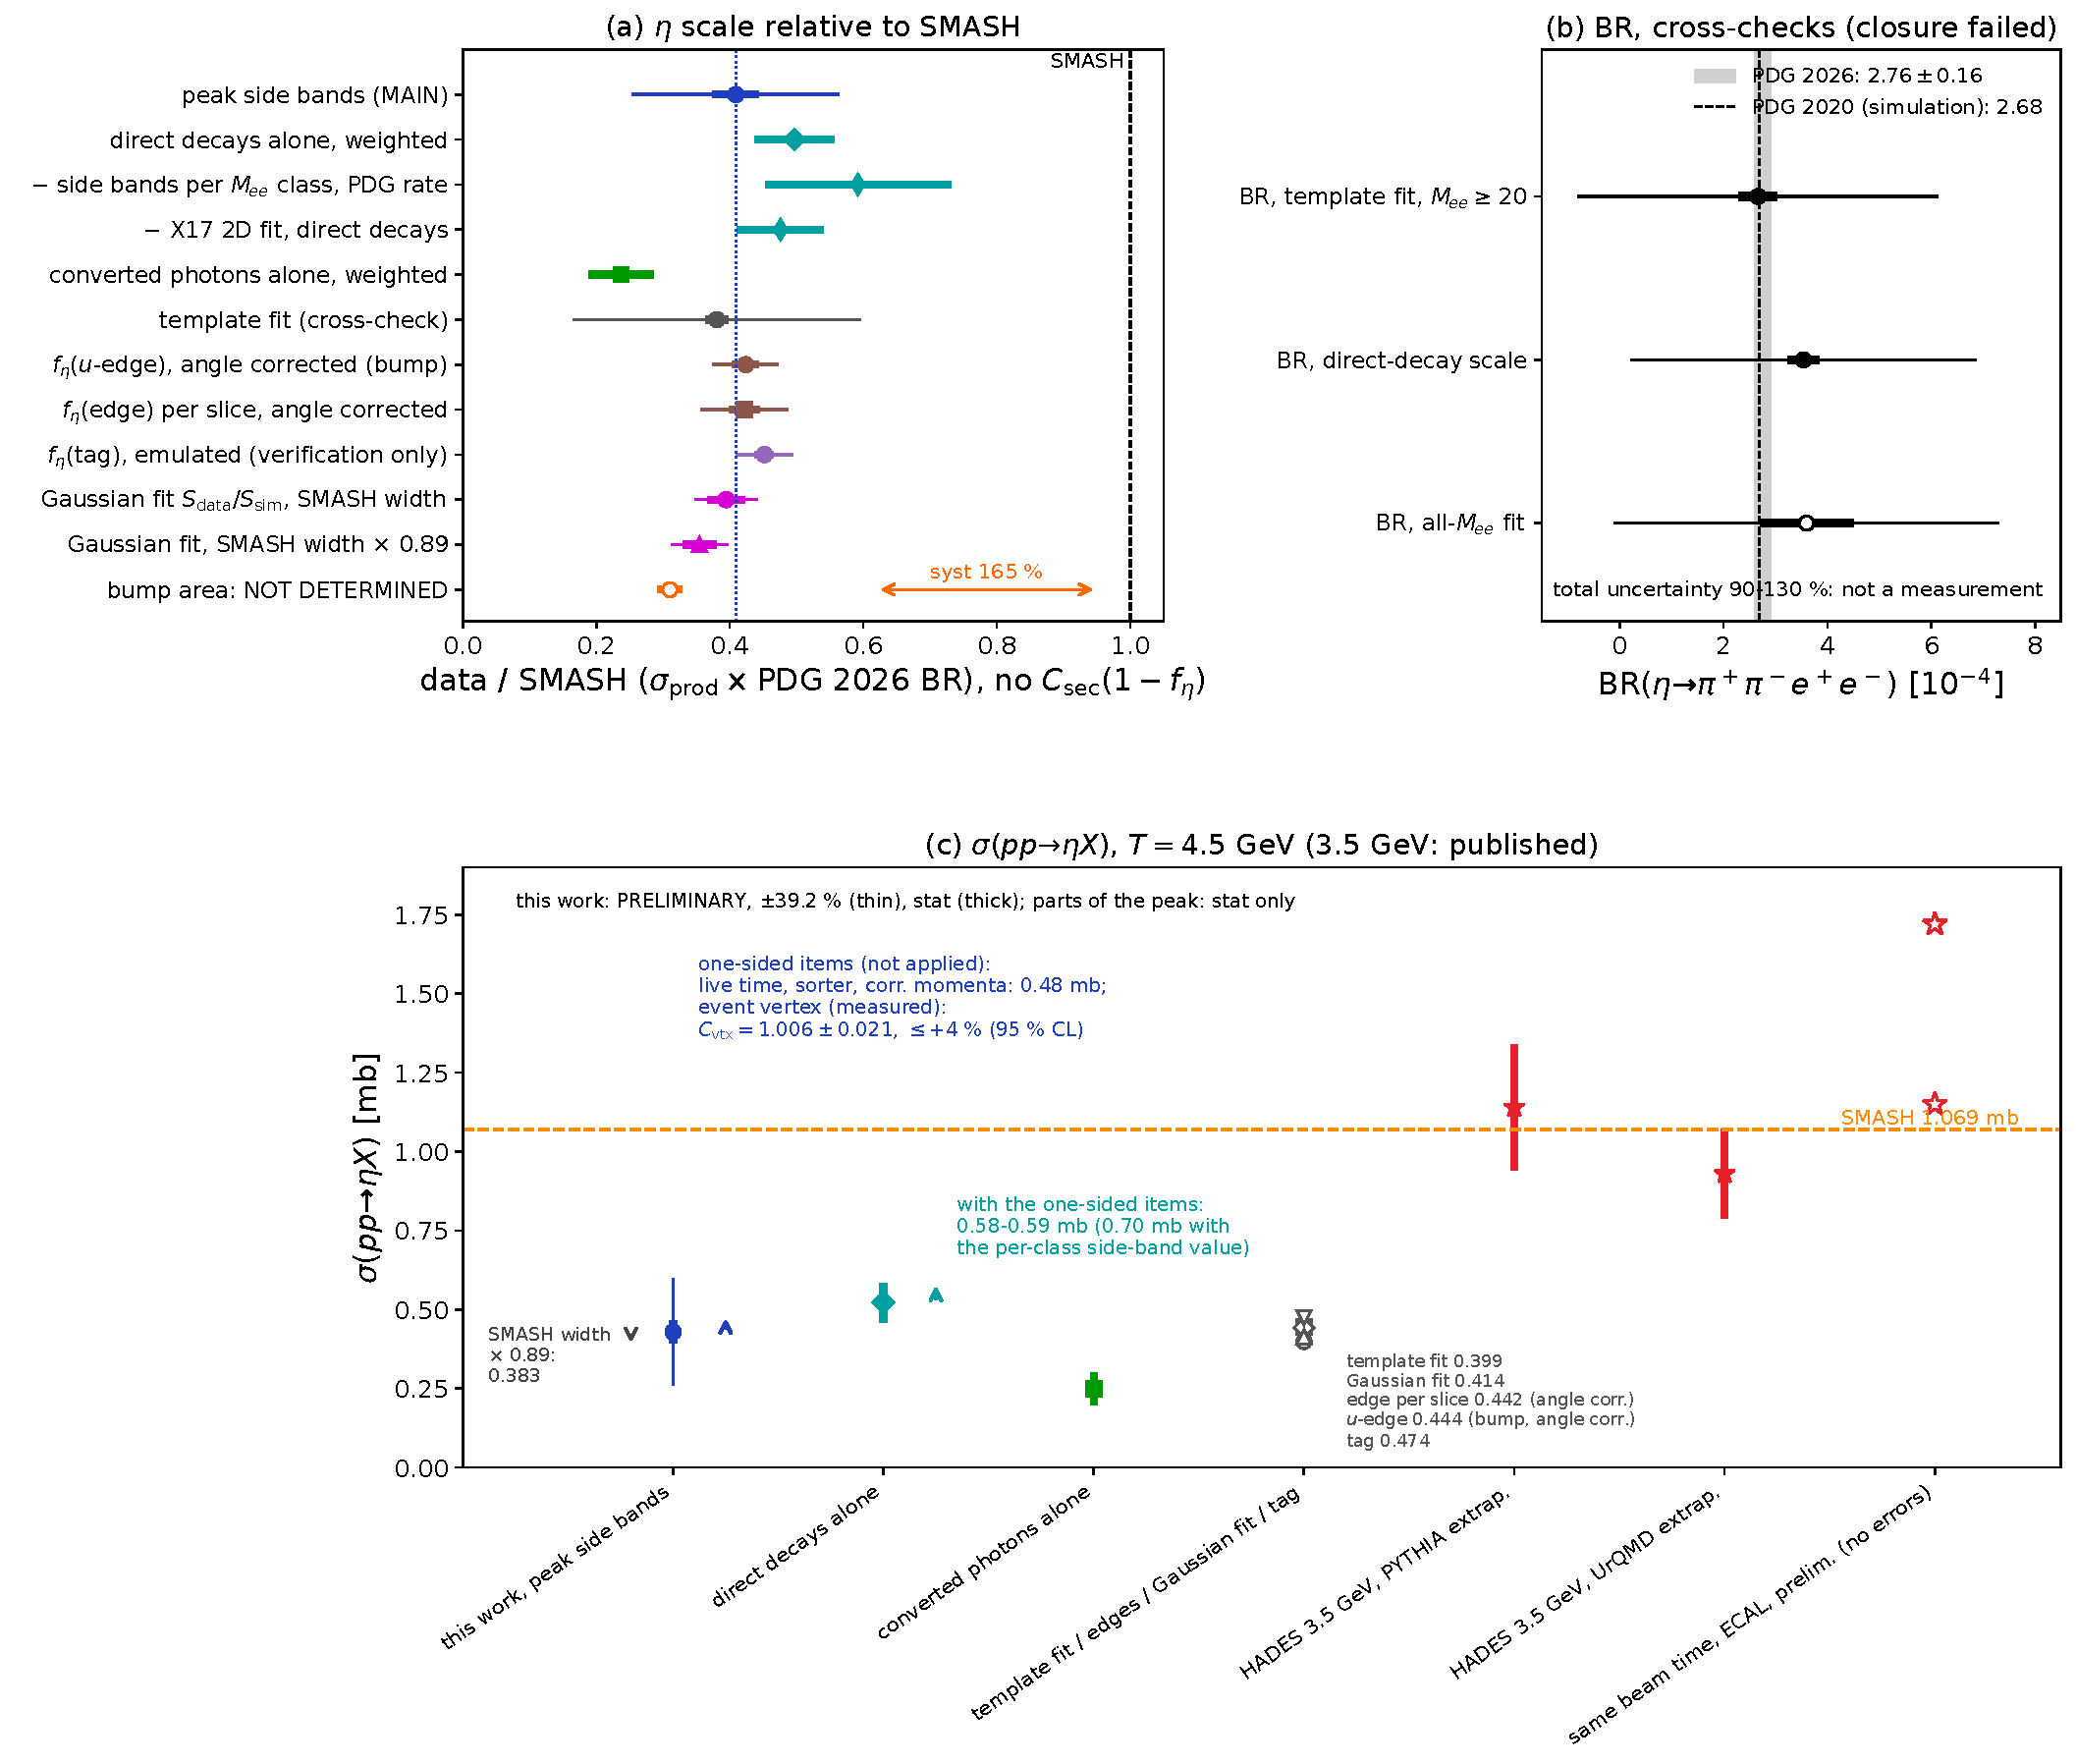
\includegraphics[width=0.76\textwidth]{figs_all/fix2_P1abc_v4_plain4.pdf}
\caption{\textbf{What it shows: \sigeta is about 0.4 of SMASH, below the HADES values at 3.5\,GeV.}
(a) $\eta$ scale data/SMASH from every method, with the PDG 2026 branching ratios (peak 0.409; the tables quote 0.418, with the PDG 2020
values of the simulation), without the trigger-loss and target-wall corrections: the main result (peak side bands), the two parts of the
peak (each the weighted mean of the side bands per \Mee class and of the X17 fit), the template fit, the Gaussian fit of the peak (SMASH
width, and narrowed by 0.89 to the data width), the ECAL-tagged bump (verification only), the bump edges (\piz Dalitz decay angle corrected)
and the background-subtracted bump area (not determined); thick bars statistical, thin bars total. (b) BR$(\eta\to\ppee)$ from the template fits
(cross-checks: they failed the pseudo-data test; open marker: a fit of both \Mee classes, not determined) against PDG. (c) \sigeta
(preliminary) with the two parts of the peak (statistical errors only), the cross-checks and the corrections not applied (arrows and blue
text: trigger live time, events lost in the START-based track sorter and counts without corrected momenta raise it to 0.48\,mb; the data peak
width lowers it to 0.383\,mb), against the published HADES values at 3.5\,GeV (PYTHIA and UrQMD extrapolations) and the unpublished values
of the same beam time (open stars, no errors).
\Sel data: \selnom; \cbsel; \lumisel. SMASH: \smashsel. Each method in its own windows: peak side bands, peak window 0.53364--0.55416,
side bands 0.5250--0.5336 and 0.5542--0.5628\,\GeVcc, all \Mee (the two parts: per \Mee class, below and above 10\,\MeVcc); X17 fit, \Mfour
0.5225--0.6100\,\GeVcc $\times$ \Mee 2--62\,\MeVcc; template fits, \Mfour 0.40--0.70\,\GeVcc in \slicesfive, \Mee$\ge10$\,\MeVcc (BR also
\Mee$\ge20$\,\MeVcc); Gaussian fit, fixed Gaussian (0.5439\,\GeVcc, width 5.4\,\MeVcc) plus a second-order polynomial in
0.5225--0.6100\,\GeVcc; bump edges, $0.30\le\Mpipi<0.40$\,\GeVcc (Figs.~\ref{fig:res-edgeus}, \ref{fig:res-edges}); ECAL tag, the base selection
plus the photon cuts of Fig.~\ref{fig:res-ecals}; bump area, \Mee$\ge10$\,\MeVcc in the bump window 0.4550--0.5225\,\GeVcc (Fig.~\ref{fig:res-peaks}a).
\figlabels{$f_\eta$: bump $\eta$ scale (data/SMASH); $\sigma_{\mathrm{prod}}$: SMASH cross section; $C_{\mathrm{sec}}(1-f_\eta)$: the
trigger-loss correction times one minus the target-wall share of the $\eta$ (not applied in (a)); $C_{\mathrm{vtx}}$: event-vertex correction.}}
\label{fig:eta-summary}
\end{figure}

%----------------------------------------------------------------------
\subsection{The \texorpdfstring{$\eta$}{eta} peak}
\inshort{$5088\pm432\,(\mathrm{stat})\pm584\,(\mathrm{syst})\pm245\,(\mathrm{MC})$ counts, 0.418 of SMASH; measured.}
The peak is counted as the data in the peak window (\Mfour 0.53364--0.55416\,\GeVcc) minus the CB, minus the smooth background taken from two
side bands (0.5250--0.5336 and 0.5542--0.5628\,\GeVcc), corrected for the part of the peak that leaks into them (Fig.~\ref{fig:res-peaks}b):
$5088\pm432\,(\mathrm{stat})\pm584\,(\mathrm{syst})\pm245\,(\mathrm{MC})$ counts, $0.418\pm0.035\,(\mathrm{stat})\pm0.025\,(\mathrm{MC})$ of SMASH. The
cross-checks of the whole peak and of the bump agree (0.36--0.45 of SMASH) but share the same counts and normalisation; only the two parts of the
peak differ (0.24 and 0.50, \S\ref{sec:phys}). \emph{Measured}: of the peak methods, the side bands are the only one that recovered the known
answer on simulated pseudo-data with realistic template noise (bias 0.5\,\%); in the harder test with templates and pseudo-data from different
halves of the simulation no method passes, the side bands included ($+14$\,\% in one scenario; \S\ref{sec:closure}). The count is not comparable with
the data-only report's peak content, 4364: that fit uses another selection (both pion tracks within 40\,mm of the event vertex, missing mass below
2.85\,\GeVcc) and no factor 64/63, so the two parts are compared through the $\eta$ scale relative to SMASH.

\begin{figure}[!tbp]
\centering
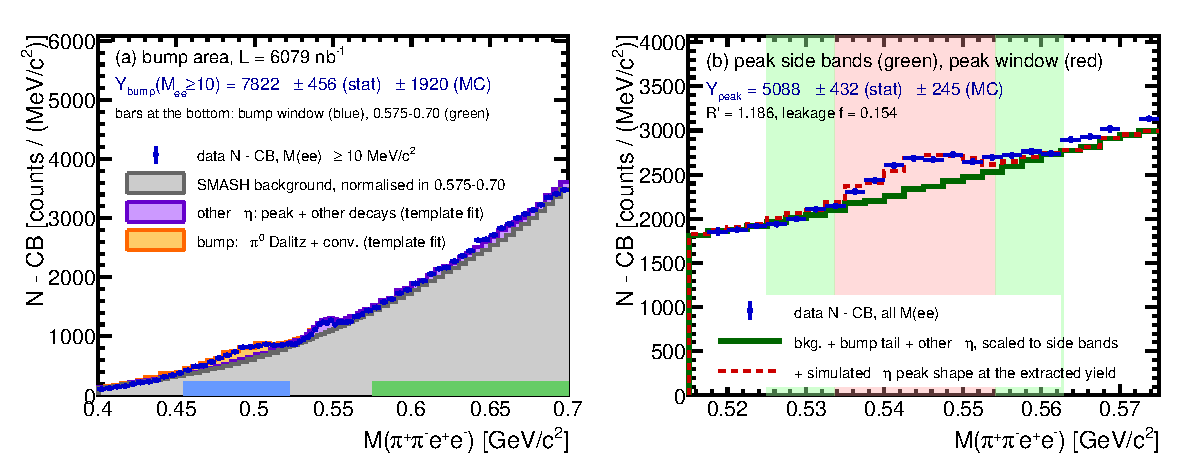
\includegraphics[width=0.80\textwidth]{figs_all/fix_wp6_E4_unrot_cnt_plain3_crop.pdf}
\caption{\textbf{What it shows: a clear $\eta$ peak (b), and the bump on a background that has to be carried down from above the peak (a).}
Data minus CB (blue), raw counts per \MeVcc. (a) The bump region, \Mee$\ge10$\,\MeVcc: grey, the SMASH background without the $\eta$, normalised
to the data in 0.575--0.70\,\GeVcc (green bar at the bottom) and carried down into the bump window 0.4550--0.5225\,\GeVcc (blue bar); violet,
the peak channels and the other $\eta$ decays, orange, the two bump channels (\piz Dalitz decay and converted photon), both at the scales of the
template fit; printed at the top: the background-subtracted bump area, 7822 counts at \Mee$\ge10$\,\MeVcc (not determined). (b) The peak,
all \Mee: peak window 0.53364--0.55416\,\GeVcc (red) and side bands 0.5250--0.5336 and 0.5542--0.5628\,\GeVcc (green); green line: the
normalised background plus the bump tail and the other $\eta$ decays, scaled to the side bands; dashed: plus the simulated peak shape at the
measured yield, 5088 counts.
\Sel data: \selnom; (a) \Mee$\ge10$\,\MeVcc, the five \Mpipi slices summed; (b) all \Mee; \cbspread. SMASH: \smashsel.
\figlabels{$Y_{\mathrm{bump}}$: background-subtracted bump area; $Y_{\mathrm{peak}}$: peak yield; $R'=1.186$: ratio of the background in
the peak window to that in the side bands; leakage $f=0.154$: share of the peak that falls into the side bands.}}
\label{fig:res-peaks}
\end{figure}

%----------------------------------------------------------------------
\subsection{The \texorpdfstring{$\eta$}{eta} bump, measured through its kinematic edge}
\inshort{one step of 21$\sigma$ at the kinematic edge; the bump is $0.426\pm0.020\pm0.034\pm0.030$ of SMASH (11.6\,\% in total); measured.}
In $\eta\to\pipi\piz$ with an \ee pair from the \piz (its Dalitz decay, or a converted photon) and the other photon lost, the four tracks never
exceed a mass limit $E$ set by kinematics alone. $E$ depends on \Mpipi and \Mee of the combination, so every bump combination has its own
edge. In the distance to it, $u=\Mfour-E(\Mpipi,\Mee)$, all edges fall on $u=0$: no simulated bump entry lies above it, and the measured $u$
is smeared by 6.7\,\MeVcc. One fit, a smooth second-order polynomial plus a smeared step at $u=0$, measures the step in the data and, in the same
way, in the SMASH bump (Fig.~\ref{fig:res-edgeus}). \emph{Result}: a step of $1305\pm62$ counts per 2.5\,\MeVcc (21$\sigma$, $\chi^2$/ndf
27.3/32); with the decay angle of the simulated \piz Dalitz decays corrected to QED by a weight per count, the bump is
$0.426\pm0.020\,(\mathrm{stat})\pm0.034\,(\mathrm{syst})\pm0.030\,(\mathrm{MC})$ of SMASH (11.6\,\%; 0.390 uncorrected); visible yield in the
bump window $21\,468\pm1003\pm1708\pm1347$ counts (3.53 visible counts per \nbinv); \sigeta from the bump $0.444\pm0.021\pm0.035\pm0.031^{+0.043}_{-0.044}$\,mb;
double ratio peak/bump $0.97\pm0.09\pm0.35\pm0.09$ (its systematic error contains the make-up of the peak). In plain words: the data hold 0.43 of
the bump that SMASH predicts, about the same fraction as in the peak (0.418), so bump and peak agree; but the agreement is a weak test, because
the peak value carries 38\,\% (39\,\% with the normalisation) and both depend on the same open question of the converted photons.
\emph{Measured.}

\textbf{How reliable it is.} The systematic error, 8.0\,\%, is led by the data/SMASH resolution ratio (4.5\,\%), the step that a smooth
background projects onto the edge (4.0), the peak term with its low-mass tail (3.4) and the CB (2.6\,\%). Pseudo-data are recovered within
2\,\% for smooth backgrounds, and the quadratic background term that moves the background-subtracted bump area by $+150$\,\% moves this result by
$-2.2$\,\%; a resolution mismatch ($+6$\,\%) or a background structure as narrow as the edge ($+8$ to $+17$\,\%) would bias it. The simulated
peak has a low-mass tail that reaches the edge in $u$; without it the result would be 6.9\,\% lower. The data allow $0.3\pm1.0$ of the simulated
tail, so it is kept as simulated with half of it as a systematic term ($\pm3.4$\,\%). The edge per \Mpipi slice (Fig.~\ref{fig:res-edges}; 0.423,
0.442\,mb, total error 15.4\,\%) agrees to 0.5\,\%. The \Mee split of the bump cannot fix the share of converted photons ($0.83\pm0.20\pm0.34$
of SMASH, consistent with 1 and with the peak's 0.48).

\begin{figure}[!tbp]
\centering
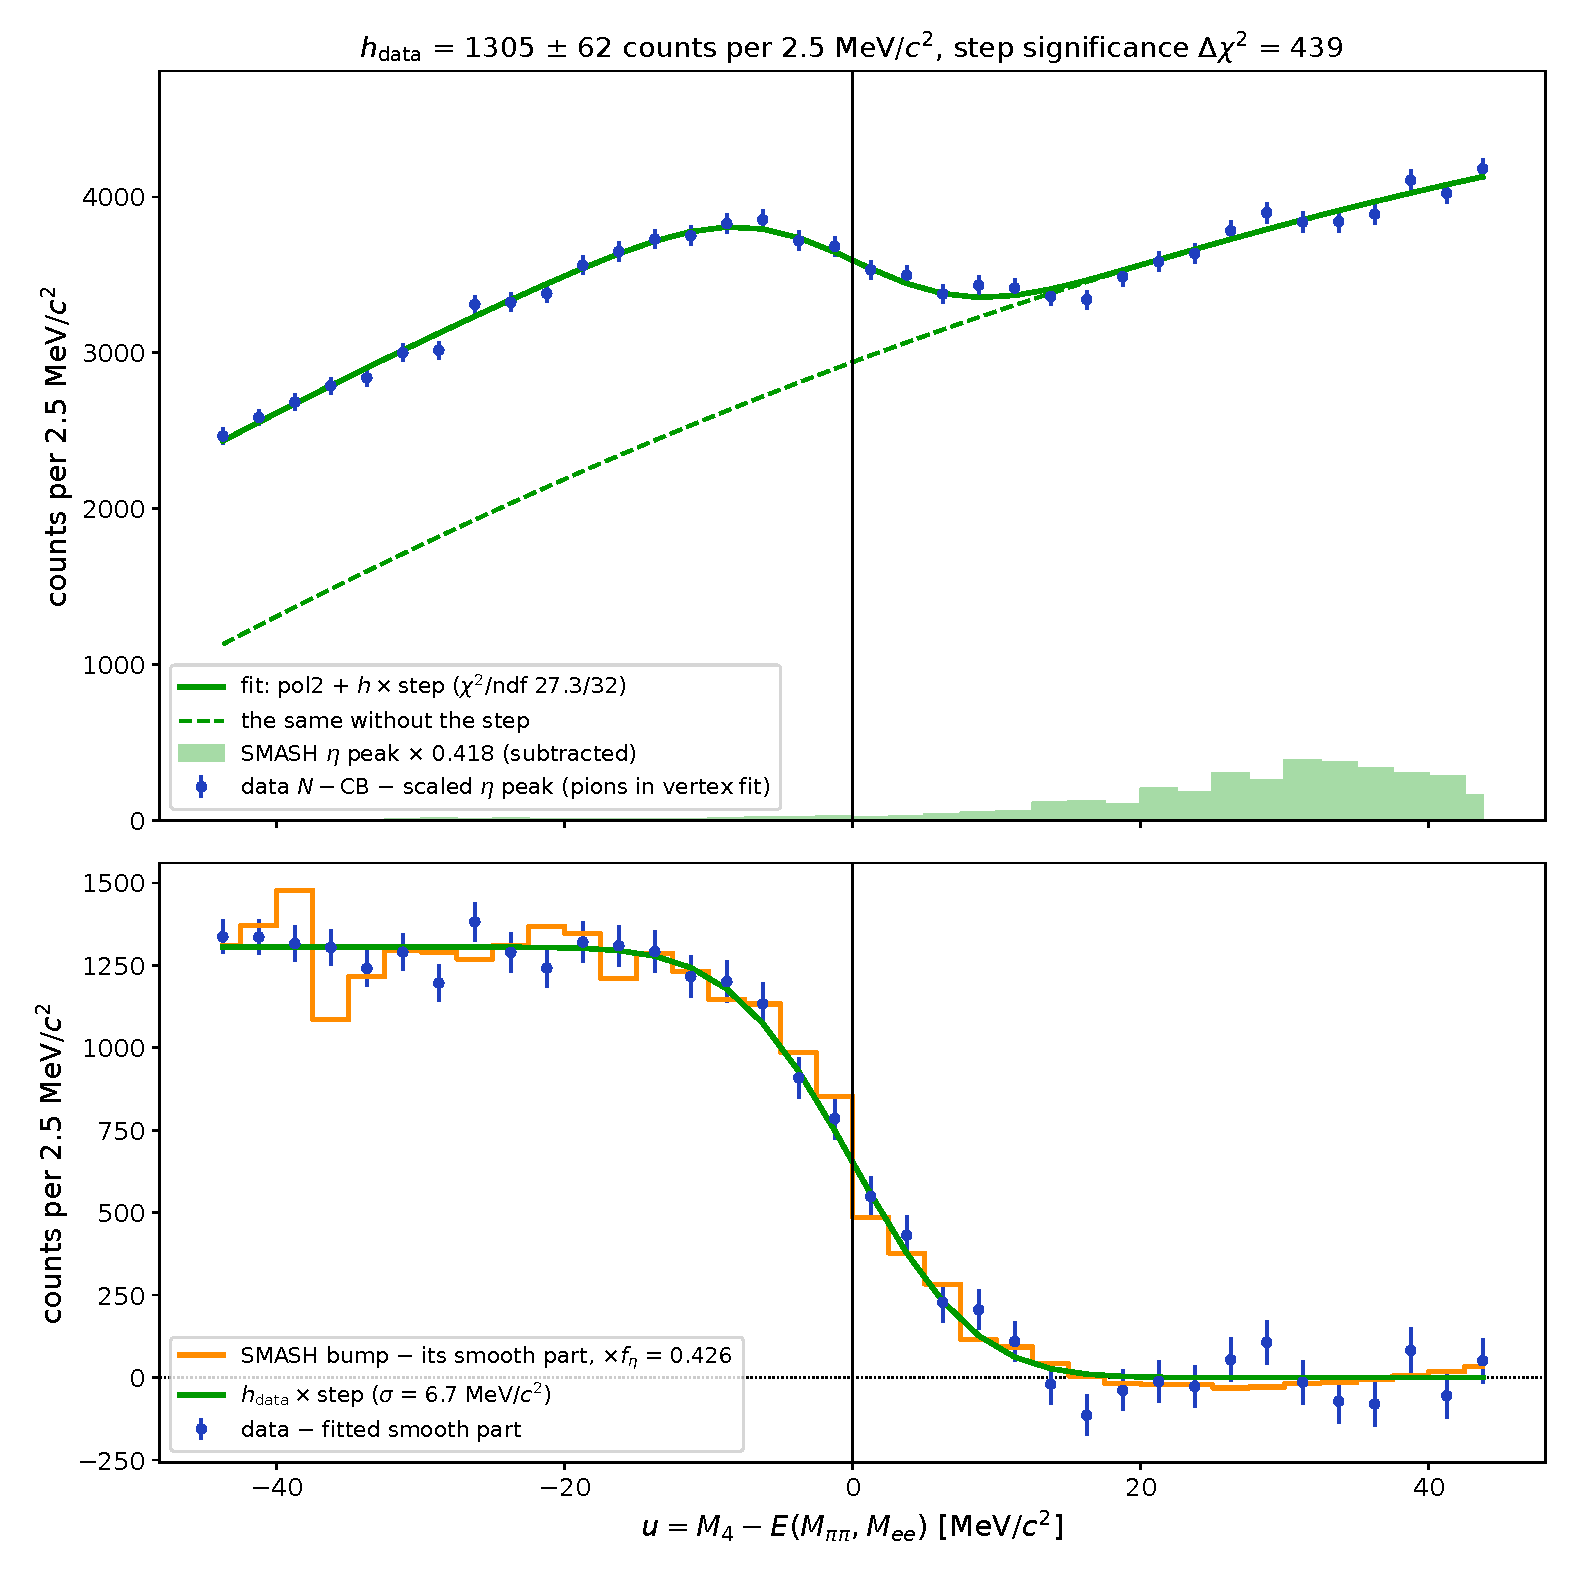
\includegraphics[width=0.62\textwidth]{figs_all/edgeu_fit_v3_plain2.pdf}
\caption{\textbf{What it shows: in the distance to the kinematic edge, $u$, the edges of all bump combinations fall on $u=0$; one fit with a smooth
part and a step describes the data ($\chi^2$/ndf 27.3/32); the step is 21$\sigma$ and has the shape of the SMASH bump scaled by 0.426.}
Counts per 2.5\,\MeVcc against $u=\Mfour-E(\Mpipi,\Mee)$. Top: data minus CB minus the SMASH $\eta$ peak scaled by its measured 0.418 (green
area, subtracted), blue; green line: the fit, a second-order polynomial plus a step at $u=0$; dashed: the smooth part of the same fit, which also
absorbs the slope of the bump below the edge, so it is \emph{not} the background. Bottom: data minus the fitted smooth part (blue); the SMASH bump
(\piz Dalitz decay angle corrected per count) minus its own smooth part, $\times0.426$ (orange); the fitted step (green, smeared by 6.7\,\MeVcc), height
$1305\pm62$ counts per 2.5\,\MeVcc.
\Sel data: \selnom; \usel; fit range $-45\le u<45$\,\MeVcc in 2.5\,\MeVcc bins; $L=6079.2\,\nbinv$. SMASH: \smashsel.
\figlabels{$h_{\mathrm{data}}$: step height in the data; pol2: second-order polynomial; $\Delta\chi^2=439$: the fit without the step is worse
by 439; $f_\eta$: bump $\eta$ scale data/SMASH; $M_4$, $M_{\pi\pi}$, $M_{ee}$: \Mfour, \Mpipi, \Mee.}}
\label{fig:res-edgeus}
\end{figure}

\begin{figure}[!tbp]
\centering
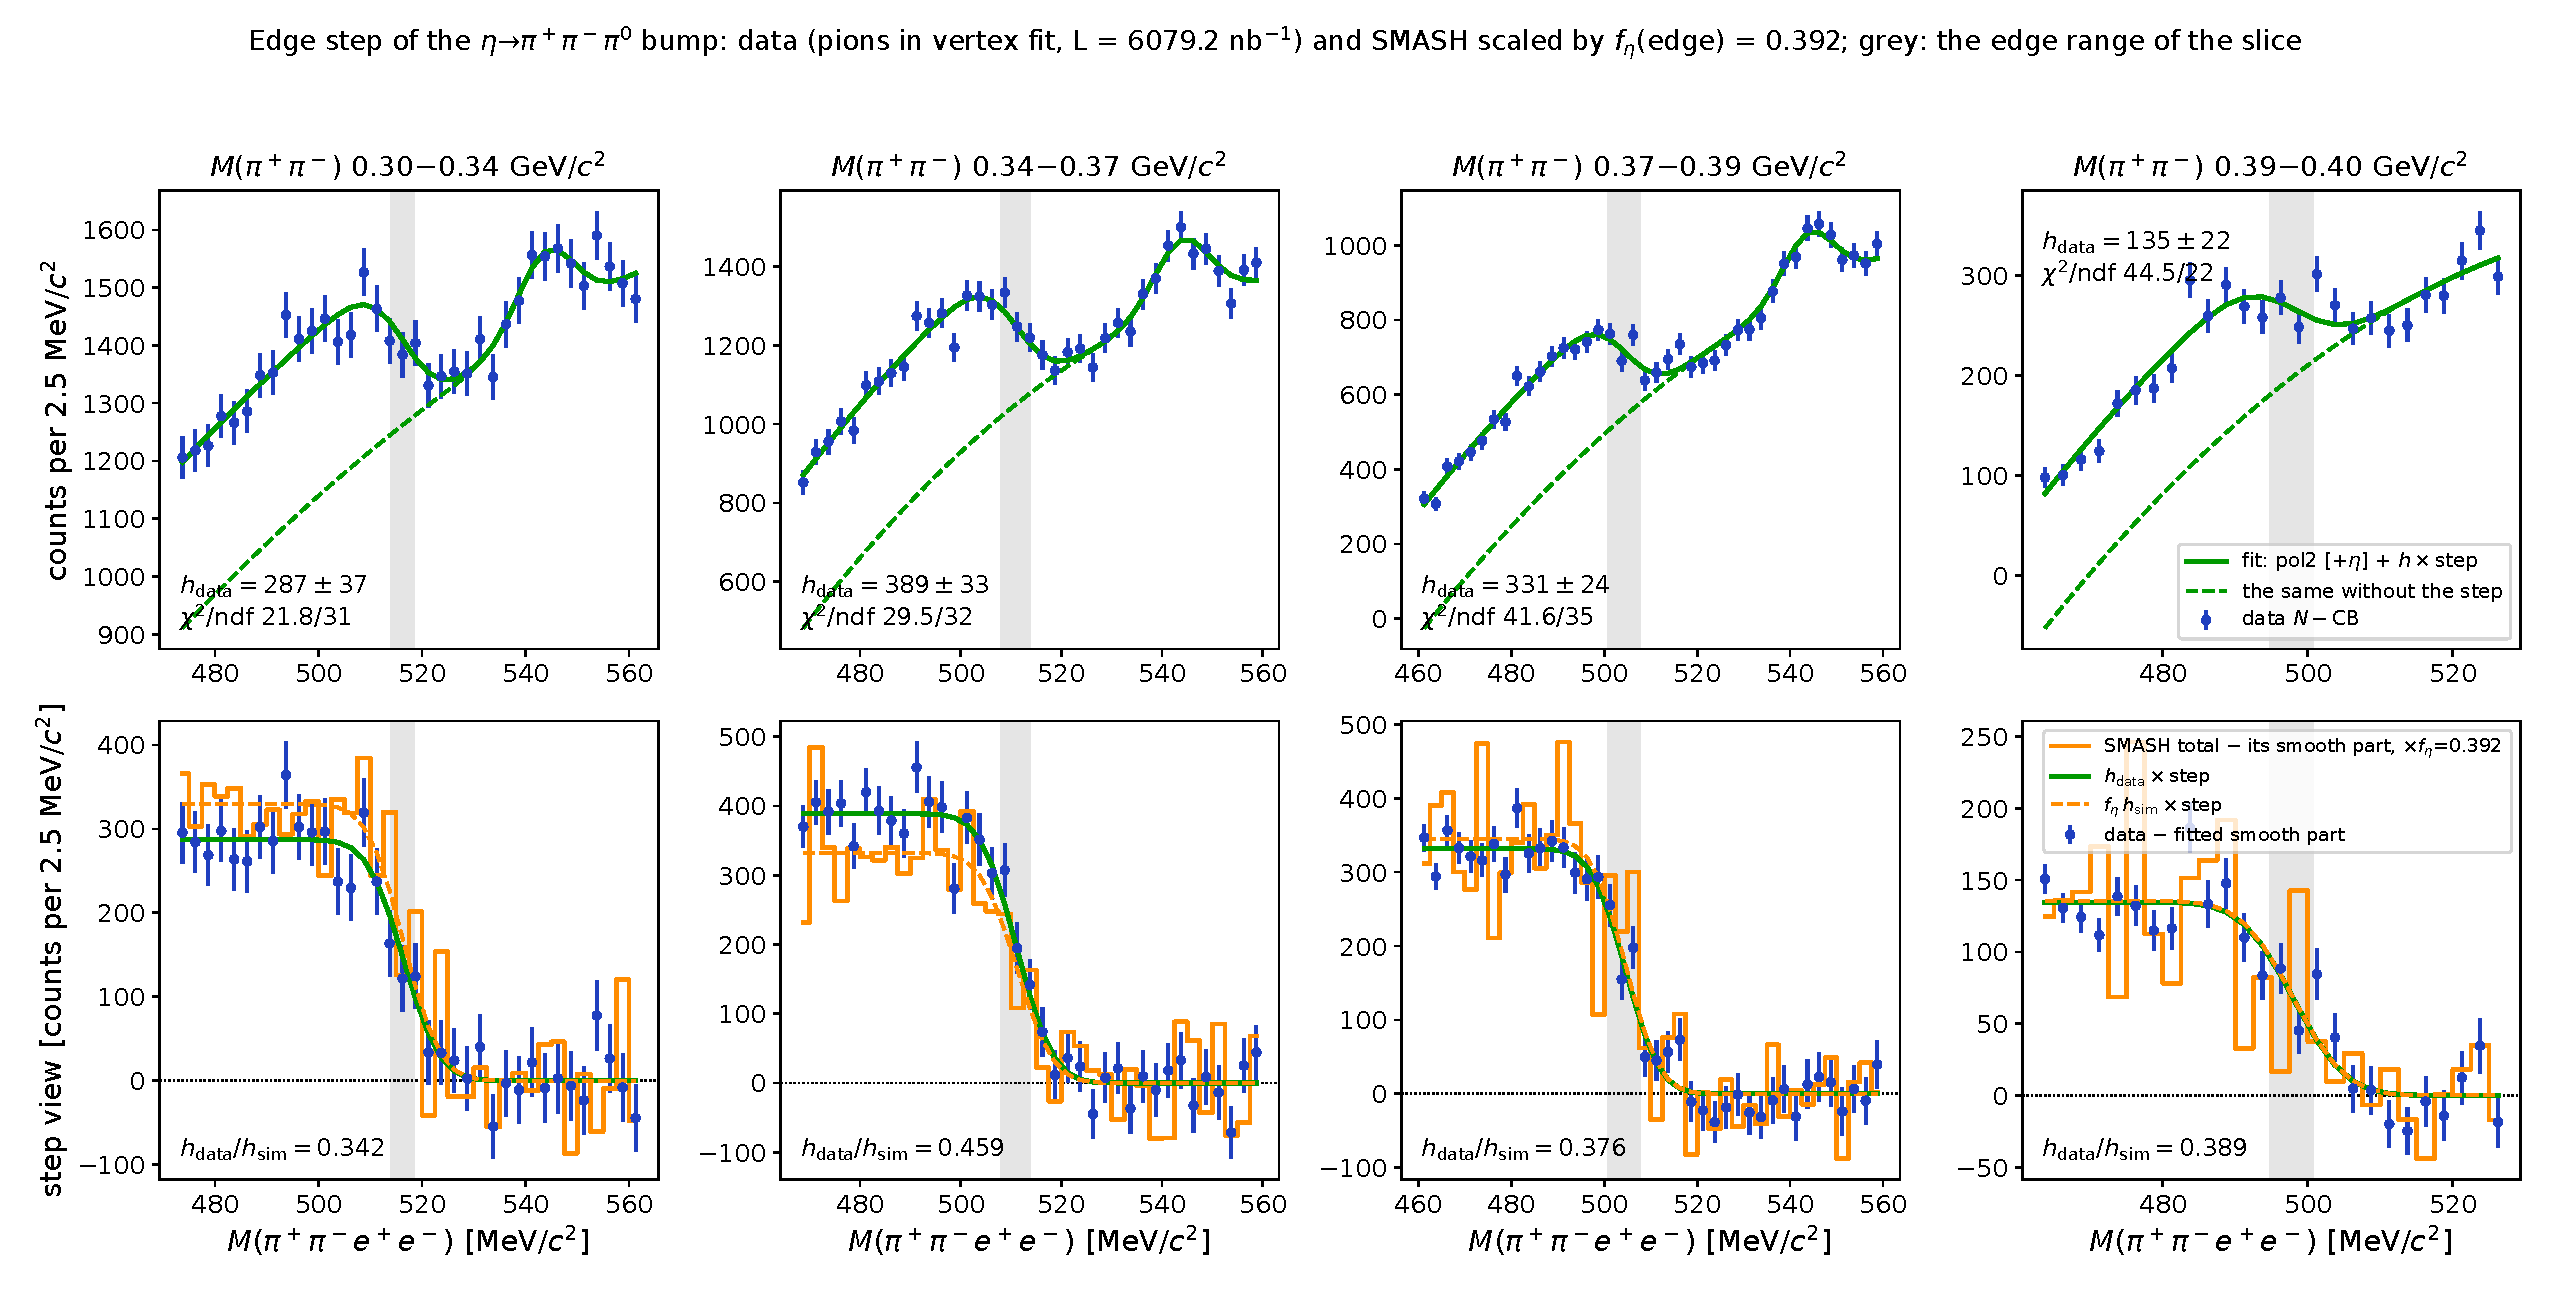
\includegraphics[width=\textwidth]{figs_all/bedge_steps_cnt_plain.pdf}
\caption{\textbf{What it shows (cross-check): the edge of the bump is seen in every \Mpipi slice, and its height in the data is 0.39 of SMASH with
the same shape.} Top: data minus CB (blue) per 2.5\,\MeVcc in four \Mpipi slices, with the fixed fit (green): second-order polynomial [+ $\eta$
Gaussian] + height $\times$ step at the edge fixed from kinematics (for \Mee$\to0$), smeared by 5.4\,\MeVcc; dashed: the same without the step.
Bottom: data minus the fitted smooth part (blue) and SMASH ($\eta$ signal and physical background) minus its own smooth part $\times0.392$ (orange
histogram; its noise is the simulation statistics); green: the data step; orange dashed: 0.392 $\times$ the SMASH step; grey: the edge range. The ratio is
uncorrected; with the \piz Dalitz decay angle corrected per count it is 0.423. Here the edge ignores \Mee and moves inside each slice; in $u$
(Fig.~\ref{fig:res-edgeus}) it does neither.
\Sel data: \selnom; all \Mee; \slicesfour; fit range the edge $\pm45$\,\MeVcc ($\pm35$\,\MeVcc in 0.39--0.40\,\GeVcc) of \Mfour; \cbsel,
from the like-sign counts of each slice; $L=6079.2\,\nbinv$. SMASH: \smashsel, the same fit.
\figlabels{$f_\eta$(edge): bump $\eta$ scale from this fit; $h_{\mathrm{data}}$, $h_{\mathrm{sim}}$: step height in the data and in SMASH;
pol2 [$+\eta$]: second-order polynomial [plus the $\eta$ peak Gaussian]; step view: data minus the fitted smooth part; SMASH total: SMASH
$\eta$ signal plus physical background.}}
\label{fig:res-edges}
\end{figure}

\textbf{Data and SMASH side by side in $u$ (Fig.~\ref{fig:res-ucompare}).} Both have one step at $u=0$ from the bump (no
other SMASH channel has a step there), the $\eta$ peak at $u=+20$ to $+55$\,\MeVcc and a smooth background that rises with $u$. SMASH as it is
does not describe the data: its bump is about 2.3 times too large and its background above the peak too low ($\chi^2$/ndf 178/36). With the
measured scales SMASH reproduces the position and the width of the data step and the shape of the peak region (the size of the step is not a
test, because it was fitted to these data); at \Mee$\ge10$\,\MeVcc, where the background normalisation above the peak was fitted, $\chi^2$/ndf
is 37.0/36. Over the whole \Mee range the smooth non-$\eta$ background of the model is too high (data/model 0.76 at every $u$, 0.65 below
10\,\MeVcc): the extra scale of the conversion-pair background found at \Mee$\ge10$\,\MeVcc ($\times3.06\pm1.45$) is too large at small \Mee,
where the conversion pairs dominate. One free factor on the non-$\eta$ background gives $0.73\pm0.02$ and $\chi^2$/ndf 32.9/35; the mismatch is
only 1.6--1.9 standard deviations of the normalisation error, and the bump result is not affected (the edge fit takes its smooth part from the data).
The lepton pairs from the two different photons of the \piz (the like-sign step below) also end at $u=0$. SMASH produces such pairs, but they
are not part of the SMASH templates used here: the analysis leaves them to the CB taken from the data, which removes them from the data
together with their \ee partners, so neither side of the comparison contains them.

\begin{figure}[!tbp]
\centering
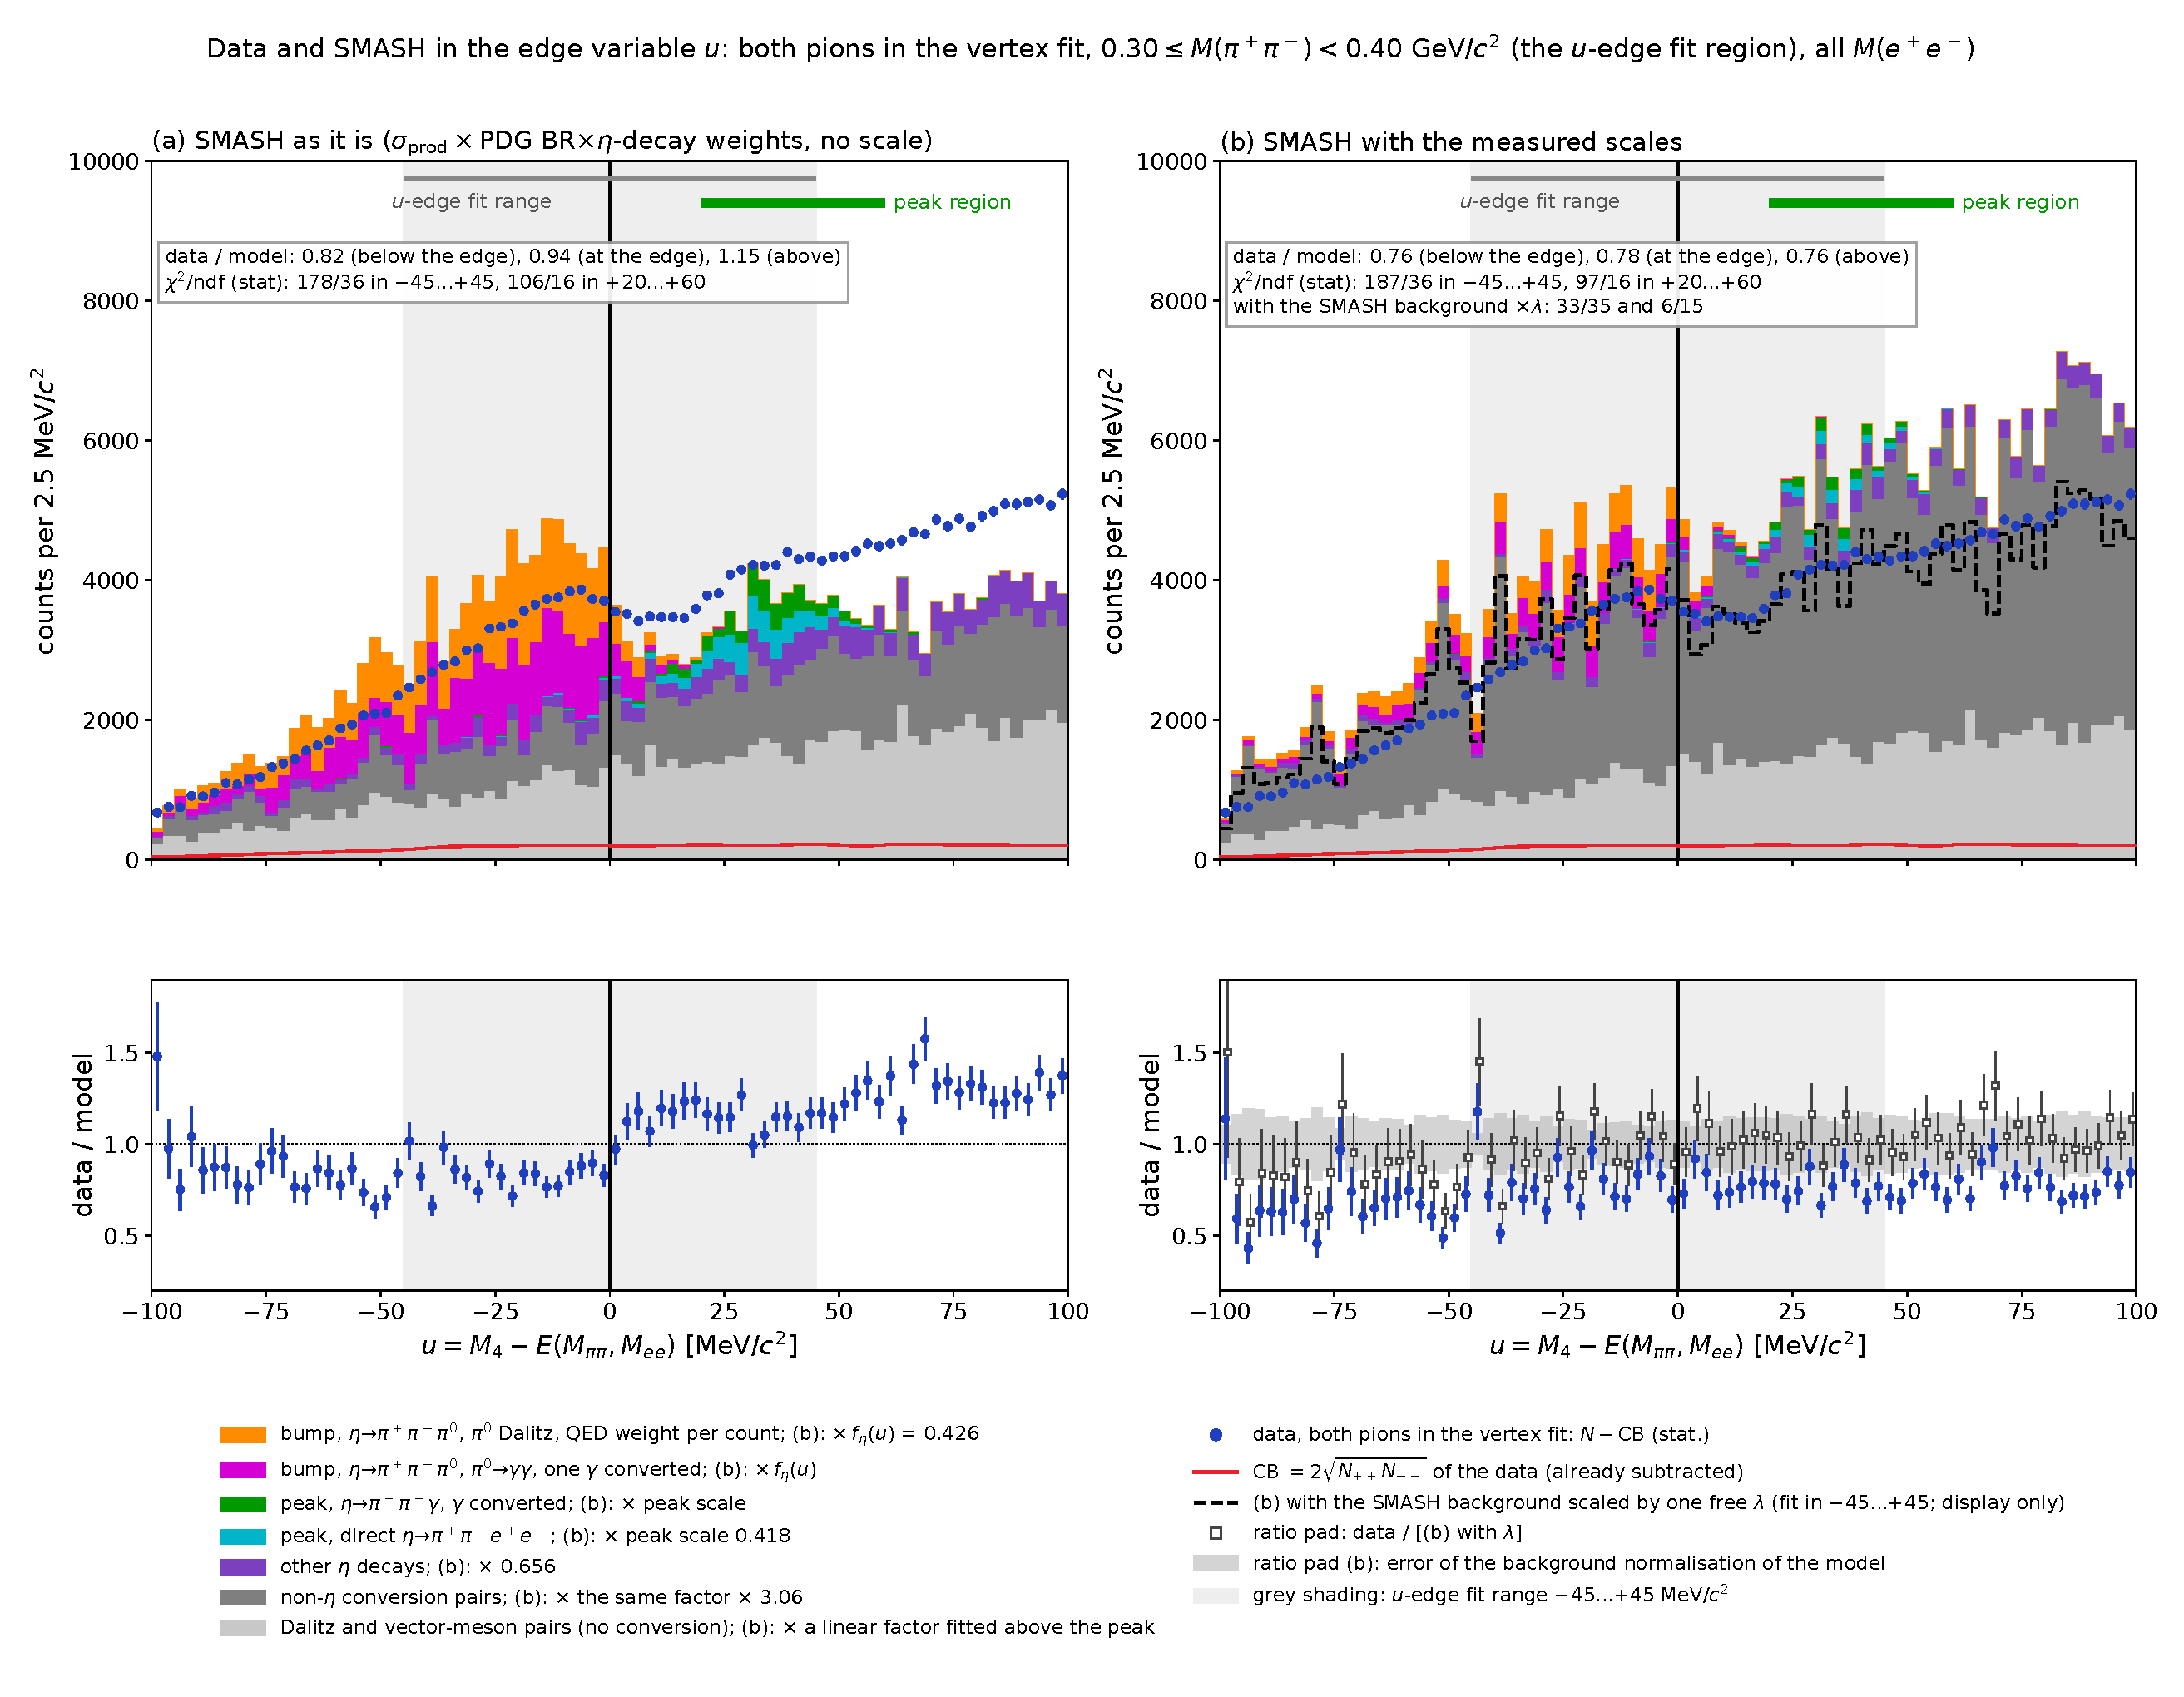
\includegraphics[width=0.86\textwidth]{figs_all/udatasim_u_overlay_plain2.pdf}
\caption{\textbf{What it shows: in $u$ the data and SMASH have the same structure (a step at $u=0$, the $\eta$ peak at $u=+20$ to
$+55$\,\MeVcc, a rising smooth background); with the measured scales (b) SMASH reproduces the data step and the peak region. The one difference
beyond the statistical errors is the level of the smooth non-$\eta$ background: the model is 1/0.76 too high at every $u$ (1/0.65 below 10\,\MeVcc;
1/0.95, within errors, above), 1.6--1.9 standard deviations of the normalisation error (grey band).}
Data minus CB (blue) in counts per 2.5\,\MeVcc; red line: the CB (already subtracted; the simulation gives no CB). Stack: SMASH in expected
counts, \piz Dalitz bump orange, converted-photon bump magenta, $\eta\to\pipi\gamma$ with converted photon green, direct decays cyan, other
$\eta$ decays violet, background with a conversion pair dark grey, background without one light grey. Lepton pairs from the two different
photons of a \piz are not part of these SMASH templates: they are left to the CB taken from the data. (a) SMASH as it is. (b) The measured
scales: bump $\times0.426$; peak $\times0.418$; other $\eta$ decays $\times0.656$ (3.5\,\% of the model); the non-$\eta$ background $\times$ the
normalisation found above the peak (a scale per \Mpipi slice with a common linear tilt, and $\times3.06\pm1.45$ on the conversion pairs); dashed: (b)
with the whole non-$\eta$ background scaled by one free factor $\lambda=0.73$ (display only). Lower pads: data/model with statistical errors; in (b) grey
band: error of the background normalisation; open squares: data/[(b) with the free factor]. Light grey shading: the edge-fit range
$-45\ldots+45$\,\MeVcc; green bar: the peak region $+20\ldots+60$\,\MeVcc. The spikes of the stack are template noise: one simulated count of the
conversion-pair background stands for about 27 expected counts, $\times3.06$ in (b), so about 84.
\Sel data: \selnom; \usel (``all $M(e^+e^-)$'' in the title means all \Mee below 135\,\MeVcc); $L=6079.2\,\nbinv$. SMASH: \smashsel; \piz
Dalitz decay angle corrected per count; the non-$\eta$ background normalised to the data in 0.575--0.70\,\GeVcc at \Mee$\ge10$\,\MeVcc.
\figlabels{$f_\eta(u)$: bump scale 0.426; $\lambda$: the one free factor on the non-$\eta$ background; $\sigma_{\mathrm{prod}}$: SMASH cross section.}}
\label{fig:res-ucompare}
\end{figure}

\textbf{A step in the like-sign counts, explained} (Fig.~\ref{fig:res-eesteps}). The $e^-e^-$ counts that make the CB also step at $u=0$:
$73.5\pm15.7$ counts (4.7$\sigma$); through CB$\,=2\sqrt{N_{++}N_{--}}$ the CB carries 39 counts of it (3\,\% of the unlike-sign step). The cause
is physics: lepton pairs from the \emph{two different photons} of the \piz in $\eta\to\pipi\piz$ (a Dalitz $e^-$ and a conversion $e^-$ of the
other photon, or two conversion $e^-$). For a given \Mee such pairs have exactly the bump's edge, and the data show just that: $57.0\pm9.1$ counts
of step (6.3$\sigma$) at \Mee$\ge90$\,\MeVcc, none below 50\,\MeVcc ($3.6\pm8.9$), where 90\,\% of the bump lies. They appear mostly as $e^-e^-$
because soft $e^+$ are accepted far less often and a photon can also give a Compton or knock-on electron, which is always negative (at
\Mee$\ge90$\,\MeVcc the $e^+e^+$ counts step by $7.3\pm4.3$). Each such decay also gives $e^+e^-$ pairs of the same kind, which the CB rule
removes, and the data agree where the bump is small (\Mee$\ge90$\,\MeVcc): data minus CB $=16.8\pm13.9$ counts of step against 16.9 expected
from the SMASH bump $\times0.426$, while a like-sign artefact without $e^+e^-$ partners would give $-19.0$ (2.6$\sigma$ away); the scale of these
pairs relative to the CB rule is $1.00\pm0.39$. A charge flip of the Dalitz $e^+$ would put the step at small \Mee: flip rate $<1.2$\,\% (90\,\% CL).
\emph{What it means:} no number changes; the data are consistent with the CB rule; the peak yield and the X17 limit are not affected. SMASH
serves only to identify the origin of the step: such pairs are not part of its templates, and the CB always comes from the like-sign data.

\begin{figure}[!htbp]
\centering
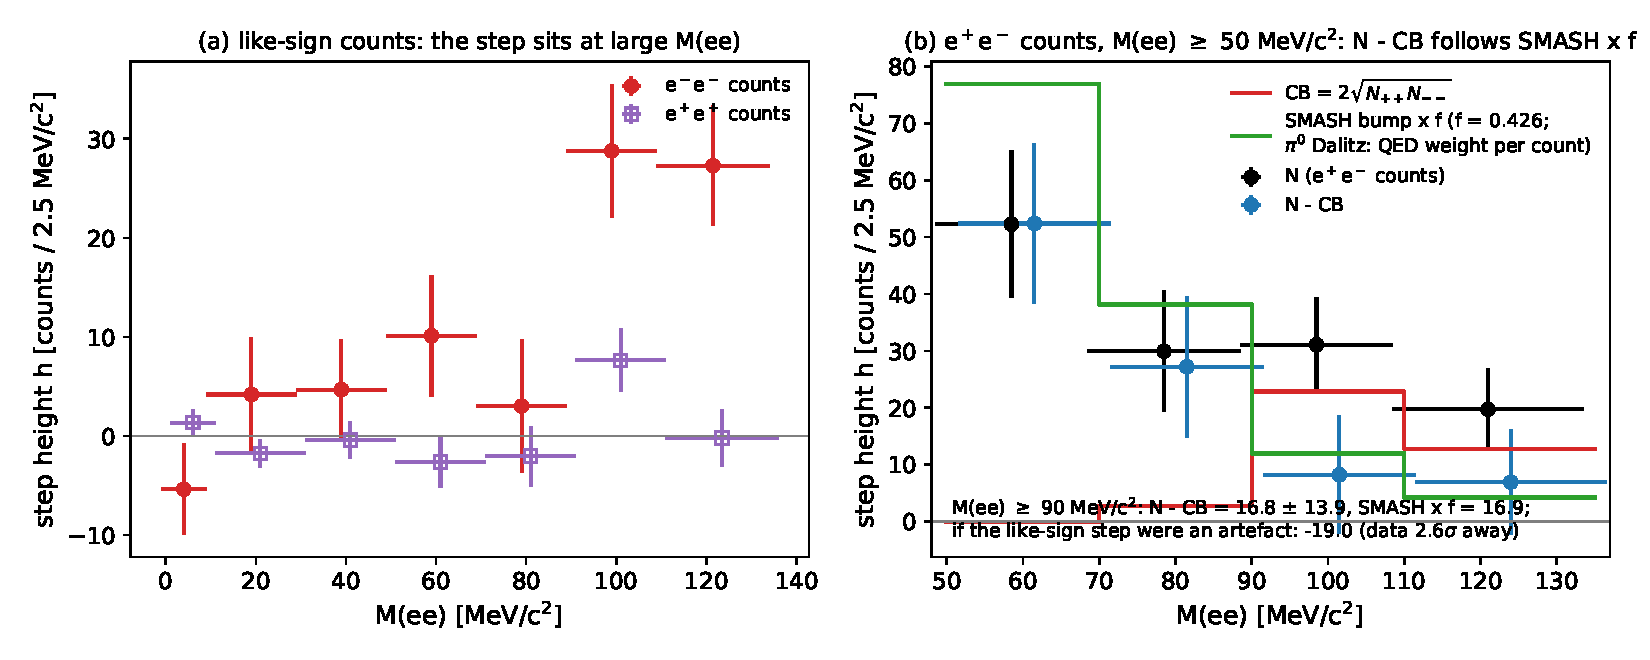
\includegraphics[width=\textwidth]{figs_all/eestep_bands_v3_plain.pdf}
\caption{\textbf{What it shows: the like-sign step at the bump edge sits at large \Mee, where the pairs from the two \piz photons lie; there the
unlike-sign counts carry the matching step, so data minus CB follows the expected bump signal, as the CB rule predicts.}
Step height at $u=0$ (counts per 2.5\,\MeVcc) of the edge fit of Fig.~\ref{fig:res-edgeus}, per \Mee band (horizontal axis). (a) Like-sign counts
of the data, no CB subtracted: $e^-e^-$ (red) and $e^+e^+$ (violet). (b) Unlike-sign counts at \Mee$\ge50$\,\MeVcc: all counts $N$ (black), the CB of each band
(red line), data minus CB (blue) and the expected bump signal, SMASH bump $\times0.426$ with the \piz Dalitz decay angle corrected per count
(green line). At \Mee$\ge90$\,\MeVcc data minus CB is $16.8\pm13.9$ against 16.9 expected; a like-sign artefact would give $-19.0$.
\Sel data: \selnom; \usel; the \Mee bands 0--10, 10--30, 30--50, 50--70, 70--90, 90--110 and 110--135\,\MeVcc, each fitted on its own
(``\Mee$\ge90$\,\MeVcc'' means 90--135\,\MeVcc); (b) CB from the like-sign counts of the same band. SMASH (green line only): \smashsel.
\figlabels{$N_{++}$, $N_{--}$: like-sign counts; $f$: the bump scale 0.426.}}
\label{fig:res-eesteps}
\end{figure}

\textbf{Not determined in the bump:} only the background-subtracted bump \emph{area} (16\,389 counts, 157\,\%): its background must be
extrapolated from above the peak (Fig.~\ref{fig:res-peaks}a), and below the bump that background overshoots the data (Fig.~\ref{fig:res-afters}).

%----------------------------------------------------------------------
\subsection{Full reconstruction of the bump with the ECAL photon}
\inshort{feasible: about 12\,\% of the bump as a clean peak; data/prediction 1.16 or 0.84, depending on the photon energy scale; verification only.}
The lost photon of one third of the bump combinations hits an active ECAL module (one ECAL sector is off, in the data and the simulation
alike), but it is soft, so a full reconstruction keeps about 12\,\% of the bump, as a clean peak (statistical error 3.2\,\% against 5.4\,\% for
the edge). The data hold $1.16\pm0.21$ of the predicted number of tagged $\eta$ with the simulated photon energy scale and $0.84\pm0.15$ with a
data-like one (errors overestimated), one factor at every \Mpipi (Fig.~\ref{fig:res-ecals}); the $\eta$ scale from the tag (0.454) therefore
stays verification only. It needs the photon energy scale and resolution in the data (about 17\,\% high) and the simulation (7--9\,\% low), the
module efficiency (about 65\,\% in the simulation, not explained), a photon cut that does not depend on START, and at least 10 times more
simulated $\eta\to\pipi\piz$.

\begin{figure}[!tbp]
\centering
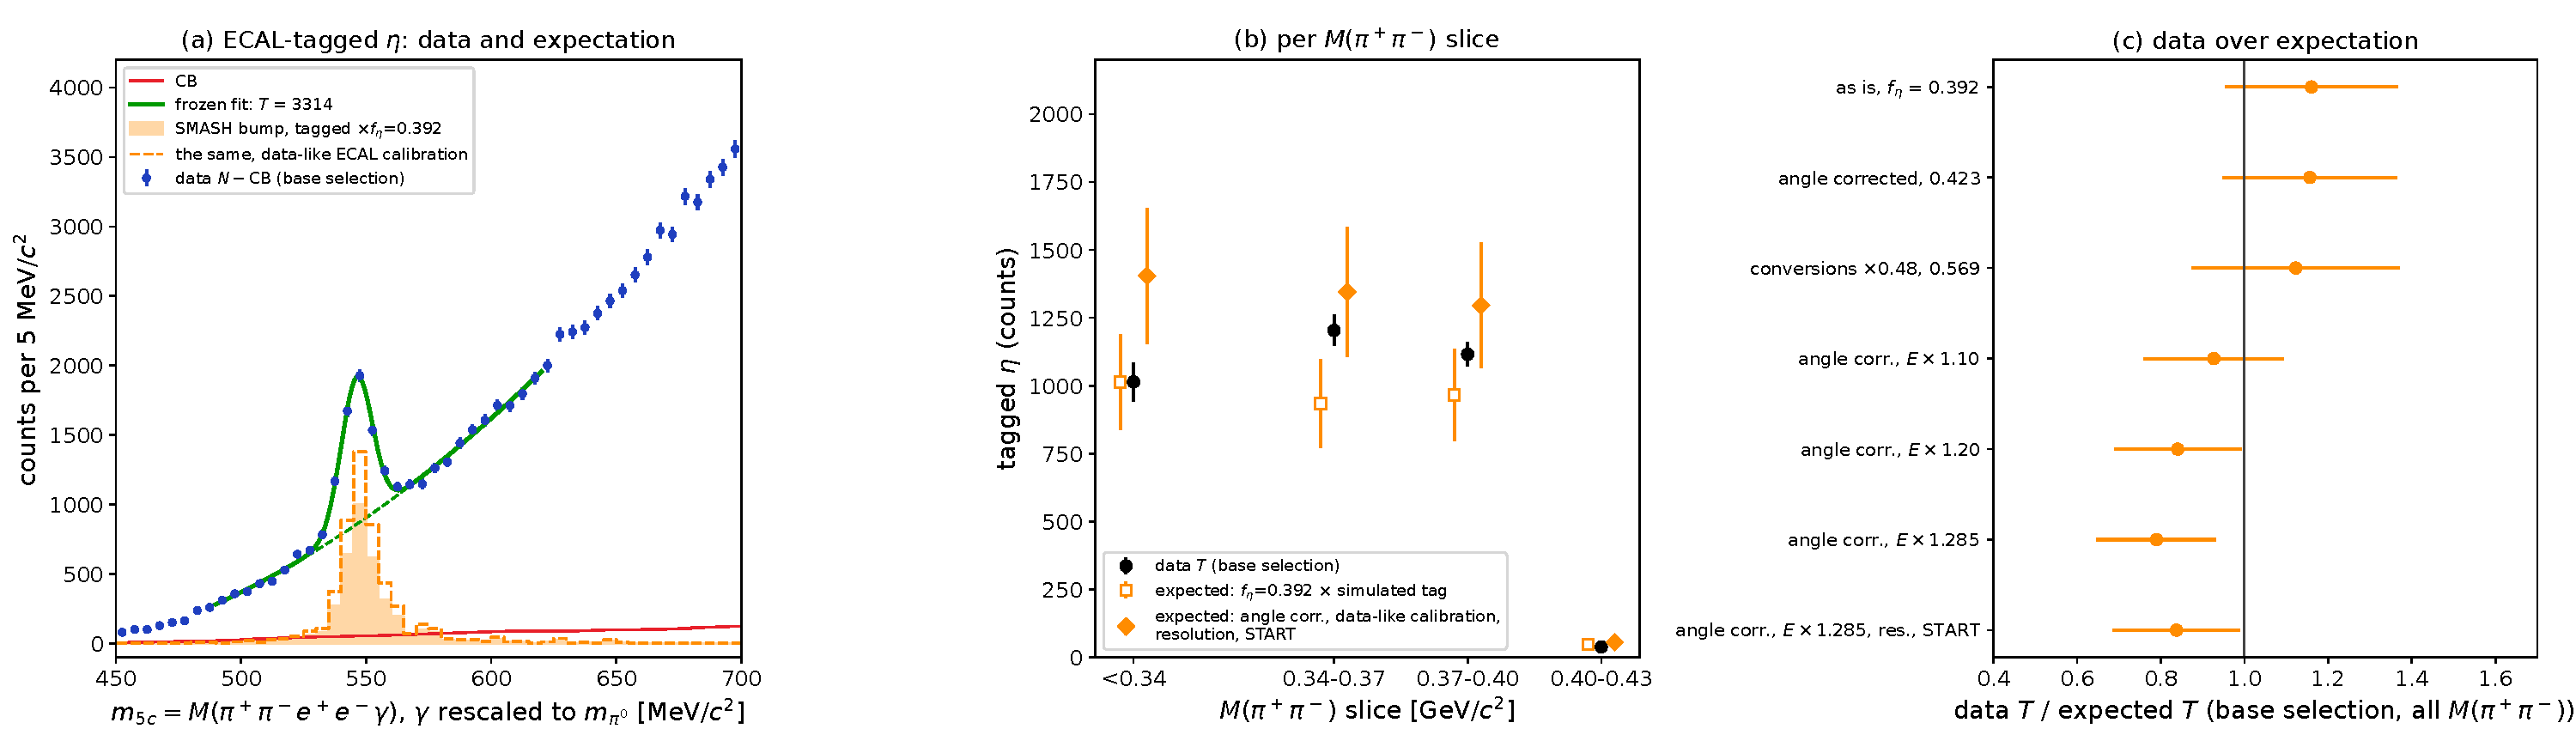
\includegraphics[width=\textwidth]{figs_all/ecalacc_tag_v3_plain.pdf}
\caption{\textbf{What it shows: the number of ECAL-tagged $\eta$ in the data agrees with the $\eta$ scale of the bump edge within the errors,
but the prediction grows by up to a factor 1.46 with the assumed photon-energy scale at the 100\,MeV threshold.} (a) Data minus CB in
$M(\ppee\gamma)$ with the photon energy rescaled so that $M(\ee\gamma)=m_{\piz}$ (blue; CB red), with the fit with fixed peak position and width
(green, 3314 tagged $\eta$); orange: the simulated tagged bump entries $\times0.392$ (bump scale per slice, uncorrected); dashed: the same with a
data-like photon calibration. (b) Tagged $\eta$ per \Mpipi slice: data (black), expected $0.392\times$ the simulated tag (open squares), best
expectation (\piz Dalitz angle corrected, cluster energies $\times1.285$, data resolution 0.964, START 0.978; diamonds); errors of the expectation:
stat $\oplus$ syst $\oplus$ MC of the scale and of the simulated tag (overestimated, both MC errors come from the same simulated entries). (c) Data
over expected for the readings of the $\eta$ scale and the assumed photon-energy scales (simulated cluster energies $\times1.10$, 1.20, 1.285): the
energy scale alone raises the prediction by up to 1.46; with the resolution and START factors the best reading is 0.84, against 1.16 as simulated.
\Sel data: \selbase (no pion-vertex condition); in addition a good ECAL photon (flagged as a photon by the ECAL reconstruction, $0.8<\beta<1.2$,
cluster energy above 100\,MeV; of several, the one with $M(\ee\gamma)$ closest to 0.140\,\GeVcc) with $0.119\le M(\ee\gamma)<0.173$\,\GeVcc and
\Mee$<0.10$\,\GeVcc; (a), (c) all \Mpipi, (b) the \Mpipi slices below 0.34, 0.34--0.37, 0.37--0.40 and 0.40--0.43\,\GeVcc; fit in 0.49--0.62\,\GeVcc
with a fixed Gaussian (0.5463\,\GeVcc, 6.2\,\MeVcc) plus a second-order polynomial; CB in 20\,\MeVcc bins; the ECAL sector at azimuth 63--117$^\circ$
is off in data and simulation. SMASH: \smashsel; the simulated bump with the same cuts and photon tag in the simulated ECAL.
\figlabels{$T$: number of tagged $\eta$; ``frozen fit'': the fit with fixed peak position and width; $f_\eta$: bump $\eta$ scale (0.392
uncorrected, 0.423 angle corrected, 0.569 with the simulated conversions $\times0.48$); $E\times$: simulated cluster energies scaled; res.,
START: data resolution and START-efficiency factors; $m_{5c}$: $M(\ppee\gamma)$ with the photon rescaled.}}
\label{fig:res-ecals}
\end{figure}

%----------------------------------------------------------------------
\subsection{X17}
\inshort{no X17 signal: $r<0.114$, i.e.\ $\BRX<3.16\times10^{-5}$ at 17\,\MeVcc (90\,\% CL$_s$, PDG 2026), about two times weaker than BESIII.}
No signal is seen (Fig.~\ref{fig:x17-mee}); the largest local excess is $0.98\sigma$ (22\,\MeVcc). The 90\,\% CL$_s$ upper limit is
\[ \mathrm{BR}(\eta\to\pi^+\pi^-X17)\,\mathrm{BR}(X17\to e^+e^-) < 3.16\times10^{-5}\qquad(m_X=17\,\MeVcc), \]
with the PDG 2026 BR$(\eta\to\ppee)=2.76\times10^{-4}$ (footnote~\ref{fn:x17pdg} gives the PDG 2020 value), against an expected (median)
limit of $2.7\times10^{-5}$ with a $\pm1\sigma$ band of 1.5--4.9$\times10^{-5}$: the data lie where the no-signal hypothesis puts them. In words:
X17 makes at most 11\,\% of the direct decays $\eta\to\ppee$ ($r<0.114$, which does not depend on the PDG edition). Across 10--40\,\MeVcc the
limit runs from $4.0\times10^{-5}$ (10\,\MeVcc) to $0.9\times10^{-5}$ (40\,\MeVcc; Fig.~\ref{fig:x17-limit}). For a vector-like X17 ($1+\cos^2\theta$) it is
$3.79\times10^{-5}$; with the X17 yield tied to the fixed $\eta$ scale of the template fit instead of the fitted direct-decay yield,
$3.29\times10^{-5}$. The procedure was fixed before the signal region (\Mee 12--28\,\MeVcc) was opened. A simple one-window count (Rolke
method) gives only $<2.6\times10^{-4}$: the shape fit is about 8 times (8.3) stronger because it measures the background instead of predicting
it (\S\ref{sec:x17}).

\begin{figure}[!tbp]
\centering
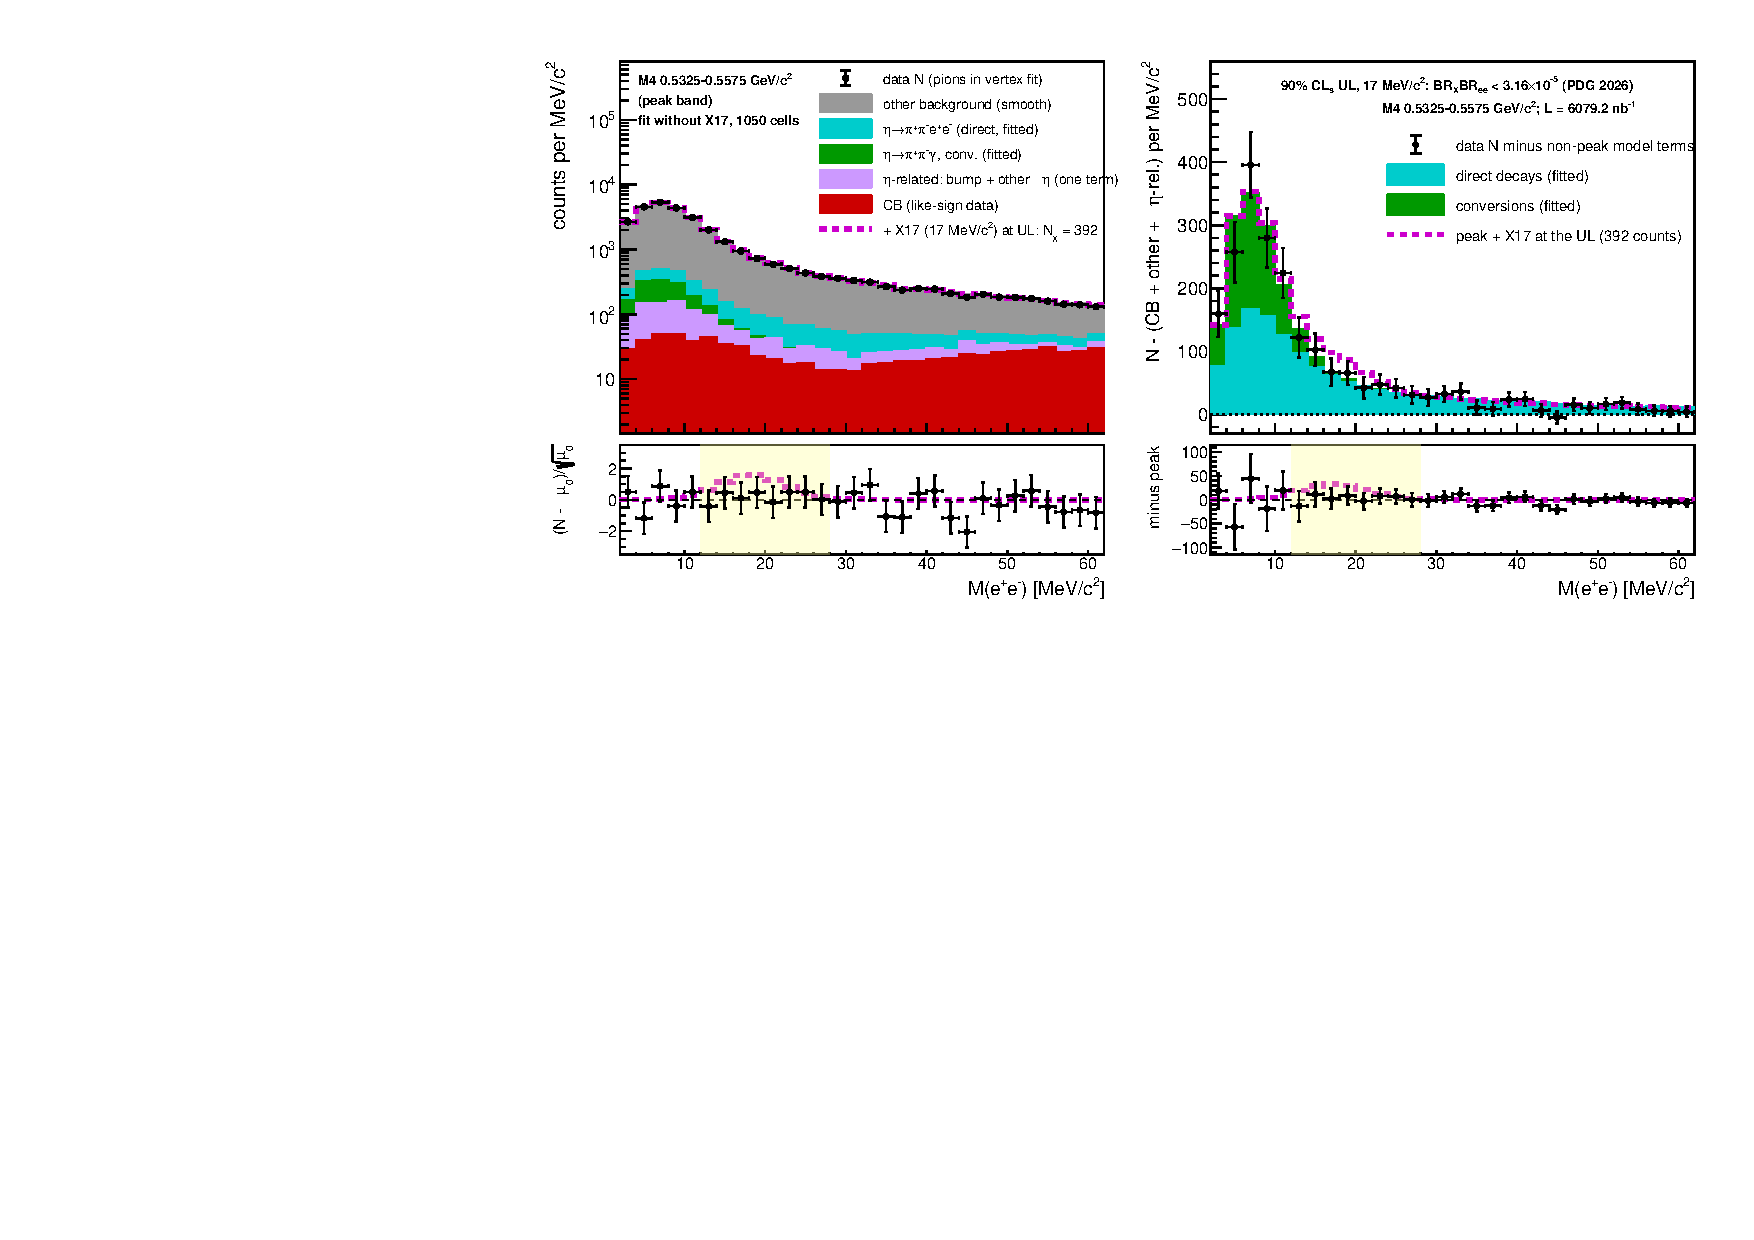
\includegraphics[width=0.90\textwidth]{figs_all/fix_X1_pdg26_cnt_plain2.pdf}
\caption{\textbf{What it shows: the \Mee spectrum around the $\eta$ peak is described without X17.} Left: data and the fixed model fitted without X17:
CB red, $\eta$-related term (the two bump channels and the other $\eta$ decays, one term) violet, $\eta\to\pipi\gamma$ with converted photon green,
direct decays cyan, other background (smooth, free in every \Mee bin) grey; magenta: plus X17 at the limit (392 counts). Right: after subtracting
the non-peak terms: data, fitted direct decays and converted photons, and these plus X17 at the limit (dotted); lower pad: residual after the
direct decays and converted photons. Yellow: the range 12--28\,\MeVcc that was hidden until the procedure was fixed.
\Sel data: \selnom; shown: \Mfour 0.5325--0.5575\,\GeVcc (the $\eta$ peak band); fitted: \Mfour 0.5225--0.6100\,\GeVcc $\times$ \Mee 2--62\,\MeVcc
(1050 cells); CB $=2\sqrt{N_{++}N_{--}}$ from the like-sign data with the same cuts; $L=6079.2\,\nbinv$. SMASH (shapes of the $\eta$ channels): \smashsel.
\figlabels{$\mu_0$: the model without X17; $N_X$: X17 counts at the limit; UL: upper limit; BR$_X$BR$_{ee}$: \BRX; $M_4$: \Mfour.}}
\label{fig:x17-mee}
\end{figure}

\begin{figure}[!tbp]
\centering
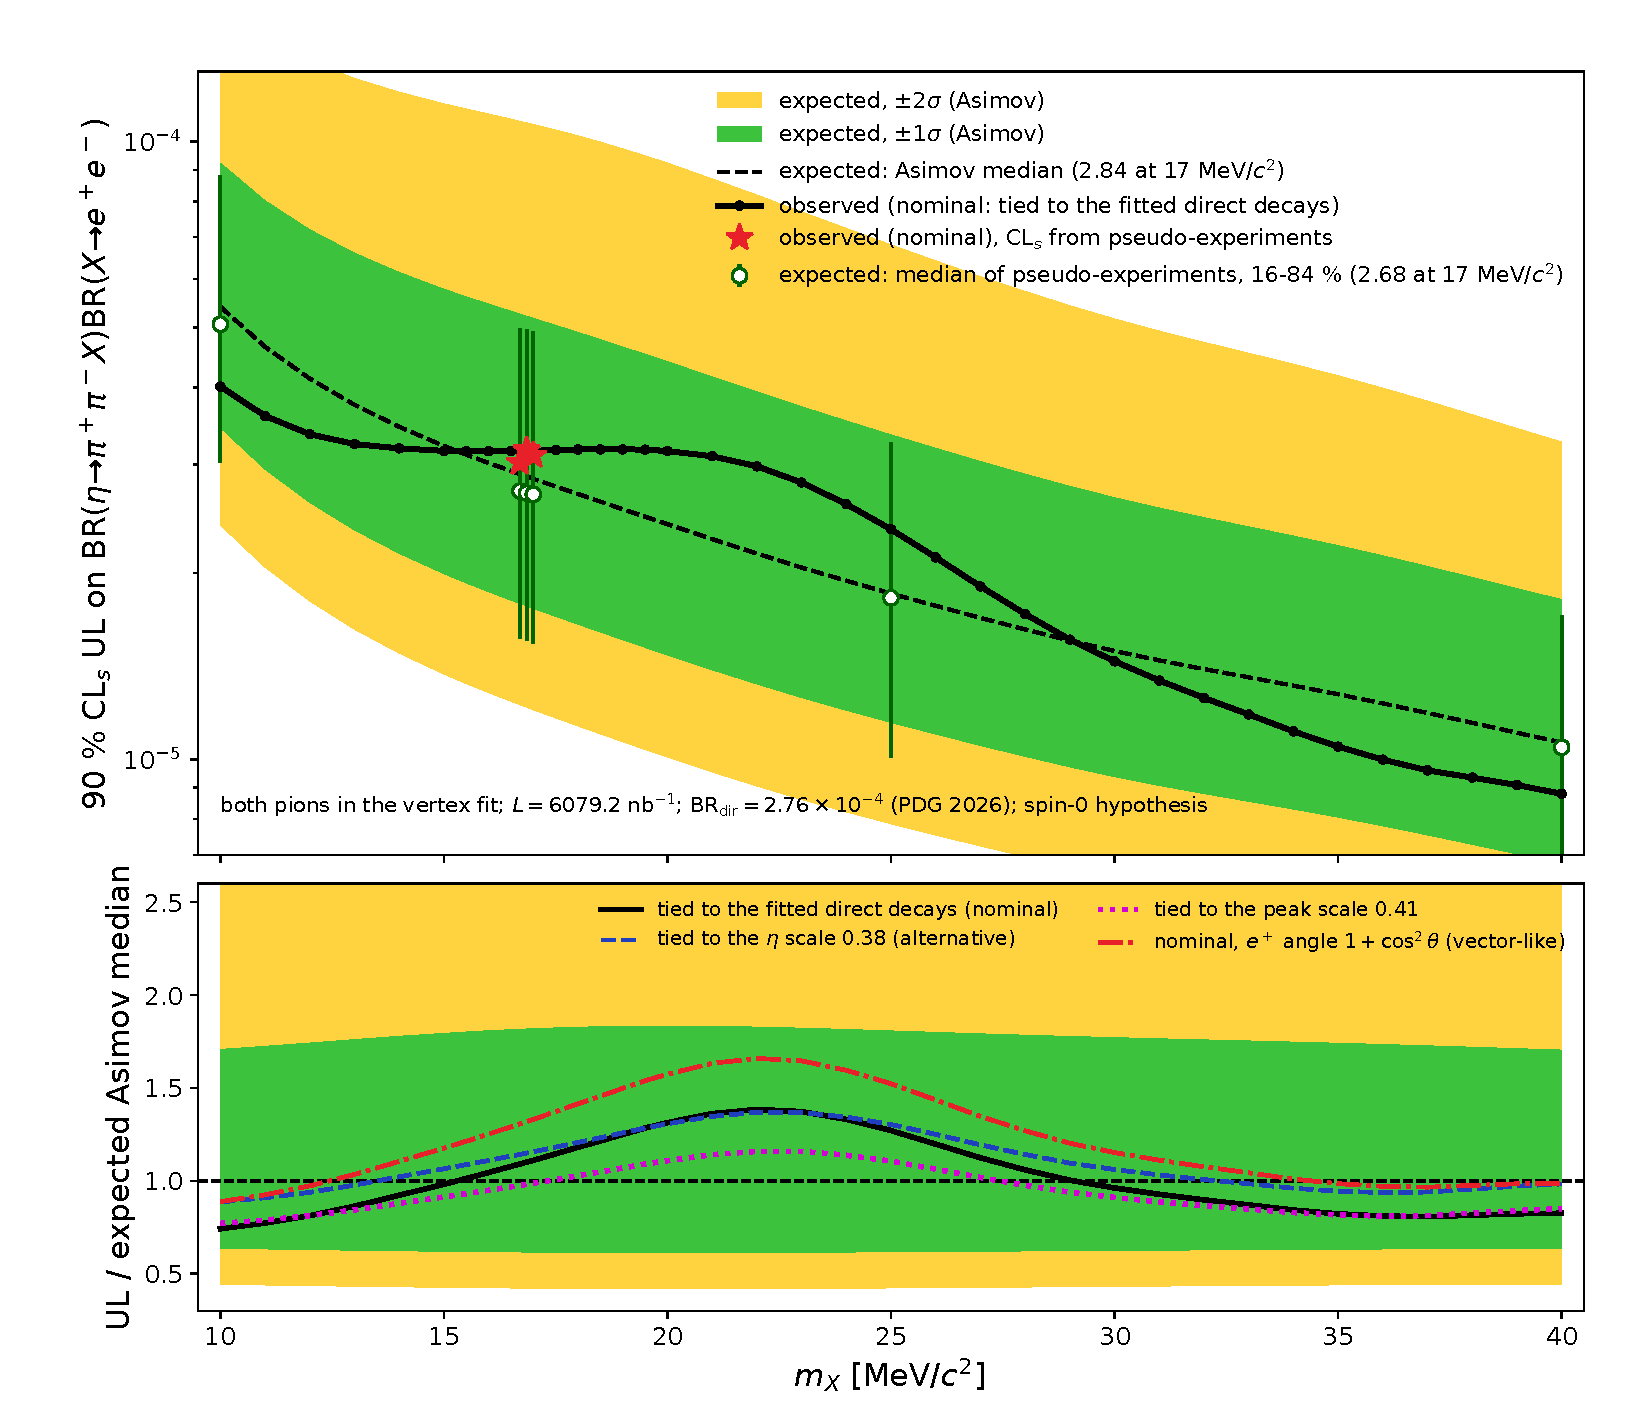
\includegraphics[width=0.70\textwidth]{figs_all/fix_X2_pdg26_plain3.pdf}
\caption{\textbf{What it shows: the observed limit stays inside the band expected without a signal at every mass.} 90\,\% CL$_s$ upper limit on \BRX
against $m_X$ (spin-0; BR$(\eta\to\ppee)=2.76\times10^{-4}$, PDG 2026): observed (black, X17 yield tied to the fitted direct-decay yield, the
nominal; red stars: CL$_s$ from pseudo-experiments at 16.7--17.0\,\MeVcc); the expectation, fixed before the signal region was opened: median of the
pseudo-data set equal to the expectation (``Asimov'', dashed, 2.84 at 17\,\MeVcc) with its $\pm1\sigma$ and $\pm2\sigma$ bands, and median of the
pseudo-experiments (circles, 2.68). Bottom: the variants relative to the expected median: the X17 yield tied to the fixed $\eta$ scale 0.38 of
the template fit (the alternative), tied to the $\eta$ scale of the peak (0.41 with PDG 2026), and the vector-like X17 ($e^+$ angle
$1+\cos^2\theta$).
\Sel data: \selnom; \Mfour 0.5225--0.6100\,\GeVcc $\times$ \Mee 2--62\,\MeVcc; CB from the like-sign data; $L=6079.2\,\nbinv$. SMASH shapes: \smashsel.
\figlabels{BR$_{\mathrm{dir}}$: BR$(\eta\to\ppee)$; UL: upper limit.}}
\label{fig:x17-limit}
\end{figure}

\textbf{Other searches} (Table~\ref{tab:x17other}). Near 17\,\MeVcc this limit is about two times weaker than the BESIII limit ($3.16\times10^{-5}$
against $0.048$--$0.053\times3.07\times10^{-4}\approx1.5\times10^{-5}$; in $r$, free of the PDG edition: 0.114 against 0.048--0.053) and numerically
similar to the HADES preliminary value from the same beam time ($2.58\times10^{-5}$). The results are built differently: CL$_s$ here against a
Bayesian limit at BESIII (a flat-prior Bayesian limit on our likelihood is $4.10\times10^{-5}$), a finer mass grid (0.5--1 against 5\,\MeVcc), $\eta$
from p+p collisions instead of $J/\psi$ decays, both spin-0 and vector-like hypotheses, and a procedure fixed before the opening. The HADES
preliminary value is an event count with the Rolke method; our own one-window count gives $<2.6\times10^{-4}$, about 10 times weaker, and the inputs
of the preliminary count are not documented here, so the agreement of the two numbers is not a cross-check. The expectation of Part~I
($1.9\times10^{-5}$) assumed that the data hold all the $\eta$ that SMASH predicts and used a counting window; it is quoted for comparison only.

\begin{table}[!htbp]
\centering
\caption{Searches for a light boson decaying to \ee in $\eta\to\pipi\ee$: 90\,\% CL upper limits. $r$, $R$: limits relative to
BR$(\eta\to\ppee)$ (here PDG 2026, $2.76\times10^{-4}$; the fixed procedure used PDG 2020, $2.68\times10^{-4}$; BESIII its own
$(3.07\pm0.12\pm0.19)\times10^{-4}$). This report: data with the nominal selection, \Mfour 0.5225--0.6100\,\GeVcc $\times$ \Mee 2--62\,\MeVcc.
BESIII: M.~Ablikim et al., Phys.\ Rev.\ D 111 (2025) 072008, arXiv:2501.10130. HADES preliminary: M.~Zieli\'nski, ``Search for the
Axion-Like-Particles in the $\eta$ meson decay with the HADES Detector'', APS GHP 2025 (Global Physics Summit), Anaheim, 15 March 2025.}
\label{tab:x17other}
\footnotesize
\begin{tabularx}{\textwidth}{@{}>{\raggedright\arraybackslash}p{2.4cm} L L L@{}}
\toprule
 & this report & BESIII & HADES, preliminary \\
\midrule
$\eta$ source & p+p at 4.5\,GeV (February 2022) & $J/\psi\to\gamma\eta$, about $1.1\times10^7$ $\eta$ & p+p at 4.5\,GeV, the same beam time \\
hypothesis & X17, spin-0 (nominal) and vector-like & axion-like particle, narrow & X17 \\
masses & 10--40\,\MeVcc, 38 masses 0.5--1\,\MeVcc apart & 5--200\,\MeVcc in 5\,\MeVcc steps & 17\,\MeVcc \\
method & 2D likelihood, CL$_s$, fixed before the opening & fit of \Mee, Bayesian & event count, Rolke method \\
limit near 17\,\MeVcc & $r<0.114$, $\BRX<3.16\times10^{-5}$ (vector-like: $3.79\times10^{-5}$) & $R<0.048$--0.053 (read off their Fig.~7,
approximate), i.e.\ $\approx1.5\times10^{-5}$ & BR $<2.58\times10^{-5}$ \\
whole mass range & $(0.88$--$4.01)\times10^{-5}$ & $R<(3.0$--$53.0)\times10^{-3}$ & -- \\
\bottomrule
\end{tabularx}
\end{table}

%----------------------------------------------------------------------
\subsection{SMASH and the data}
\inshort{SMASH does not describe the spectrum shape; 13--15\,\% of the data minus CB is target material; after the background is normalised above
the peak, the data want about 0.4 of the SMASH $\eta$.}
With nothing adjusted, data/SMASH is 0.86 in the bump window, 1.10 in the peak window, 1.27 just above the peak and 0.74 at 0.9--1.1\,\GeVcc
(one common scale: $\chi^2/\mathrm{ndf}=12$): SMASH does not describe the shape (Fig.~\ref{fig:res-befores}), and 13--15\,\% of the data minus CB
(all counts, including the $\eta$) in 0.40--0.70\,\GeVcc comes from the target material, which SMASH does not simulate (Fig.~\ref{fig:res-wallss}).
After the non-$\eta$ background is normalised to the data above the peak (Fig.~\ref{fig:res-afters}), the SMASH $\eta$ peak and bump stand out
as too high, the data want about 0.4 of them, and below the bump the background carried down overshoots the data (ratio 0.83, most bins
0.75--0.85). \emph{Measured} (\S\ref{sec:before}).

\begin{figure}[!tbp]
\centering
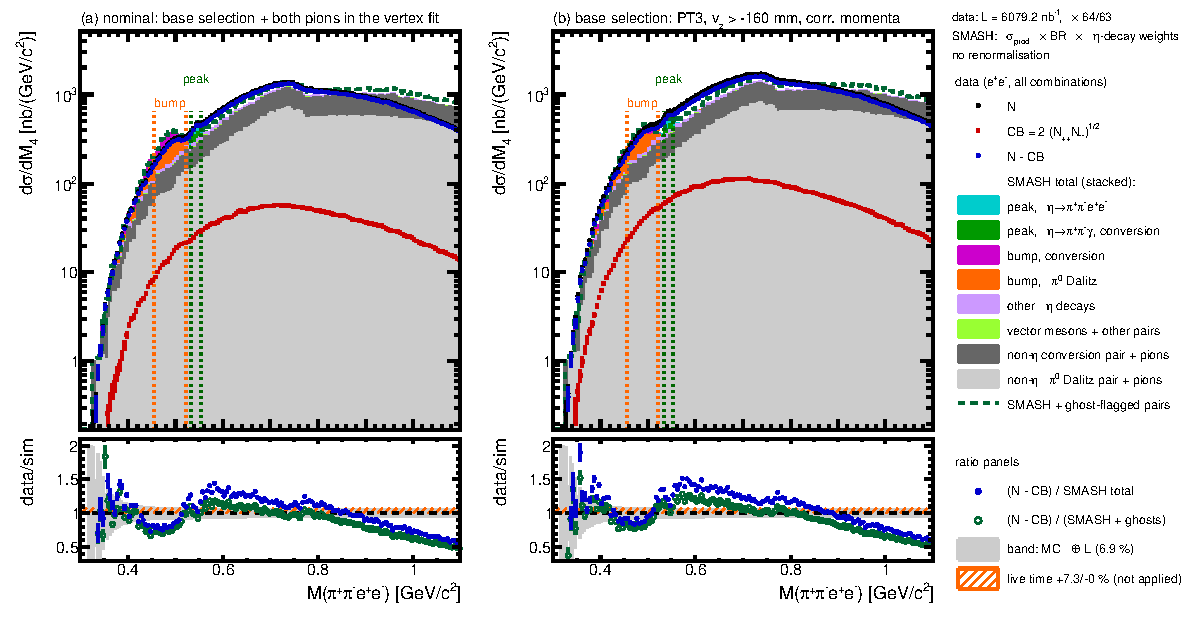
\includegraphics[width=0.92\textwidth]{figs_all/fix_B1_plain.pdf}
\caption{\textbf{What it shows: with nothing adjusted, SMASH does not describe the spectrum shape.} SMASH (stacked colours) lies below the
data just above the $\eta$ peak and above them at large \Mfour (data/SMASH from 1.27 to 0.74). \Mfour 0.30--1.10\,\GeVcc, log scale, in units
of cross section (counts per luminosity). Data: all counts $N$ black, CB red, $N-\mathrm{CB}$ blue; stacked SMASH (signal and physical
background), no renormalisation; dashed: true pairs with a track that the simulation flags as not matching one particle (ghost track), counted
as physical background. Dotted lines: bump and peak windows. Ratio panels: data minus CB over SMASH; grey band MC $\oplus$ 6.9\,\% of $L$;
hatched: trigger live time $+7.3/-0$\,\% (not applied).
\Sel (a) data: \selnom; (b) the same without the pion-vertex condition (base selection). \cbsel; \lumisel. SMASH: \smashsel.}
\label{fig:res-befores}
\end{figure}

\begin{figure}[!tbp]
\centering
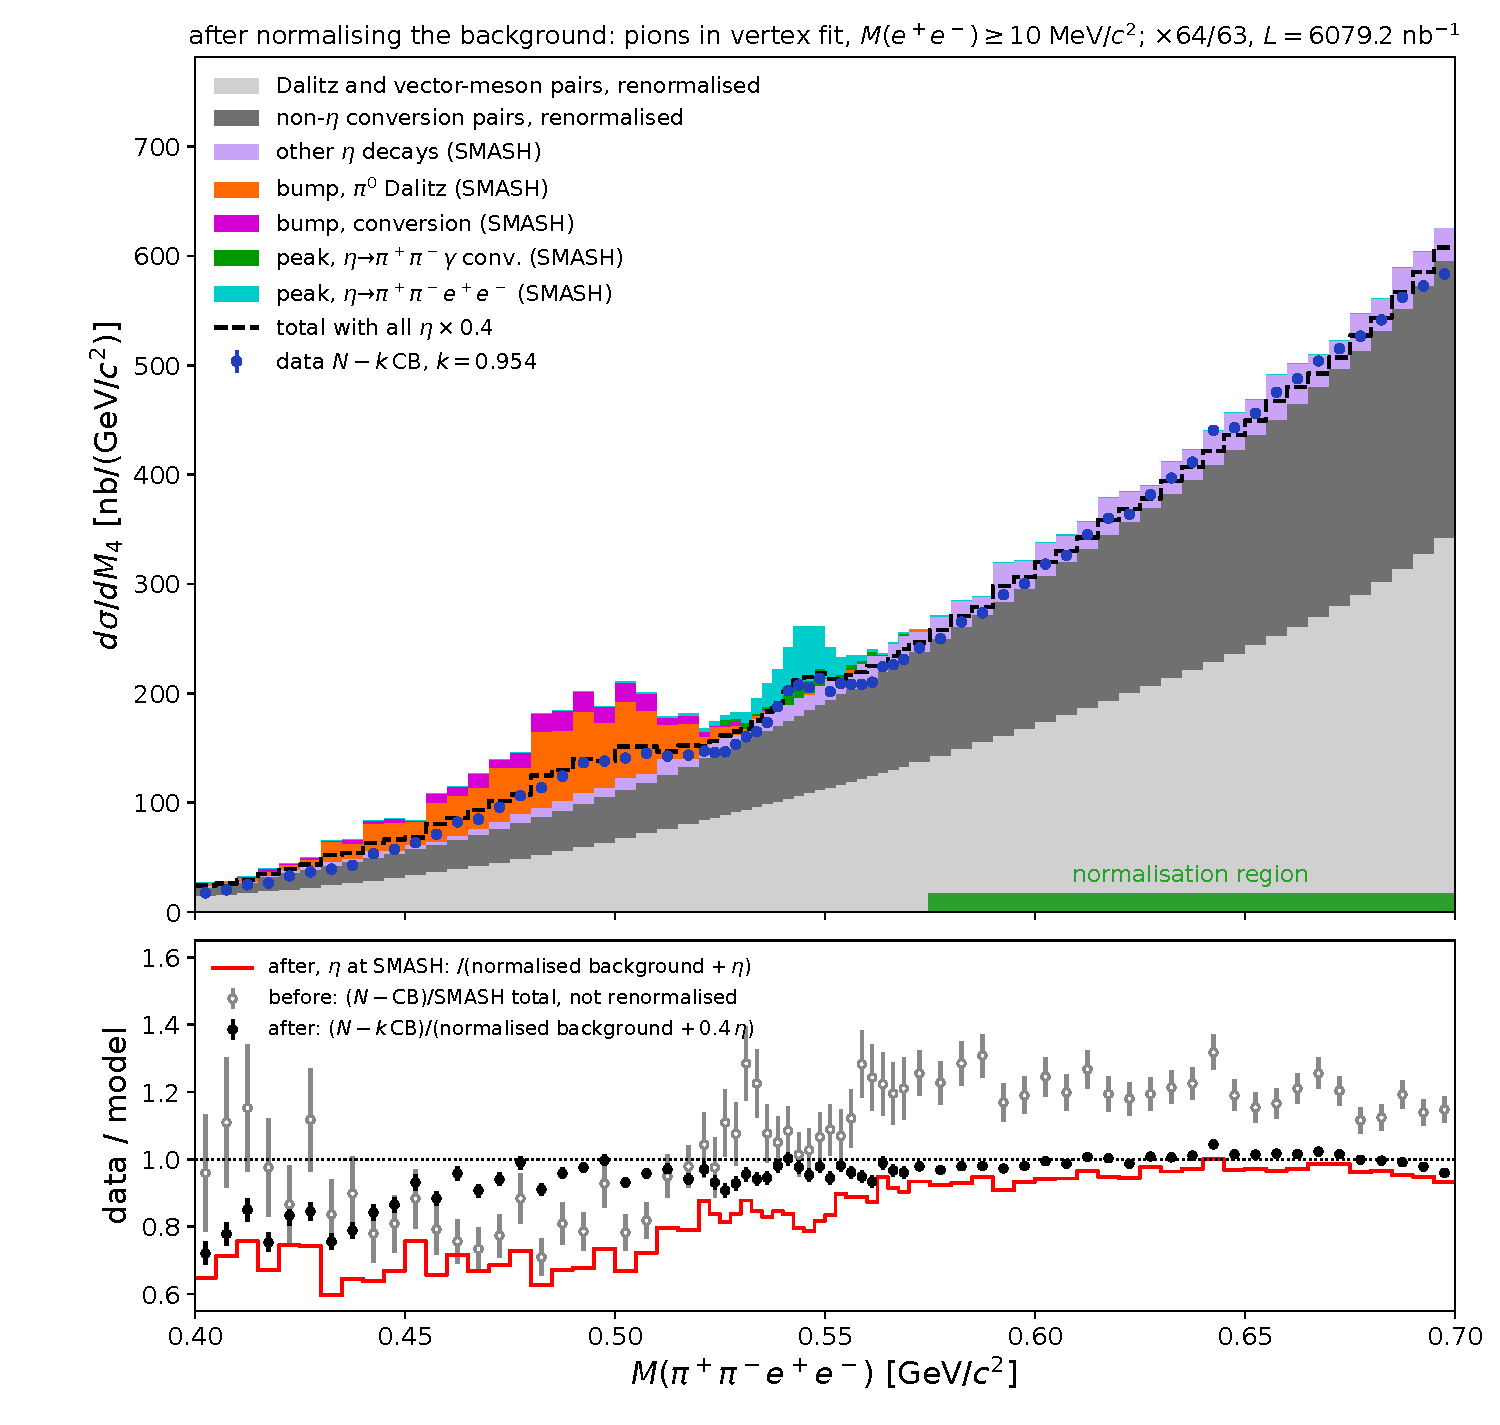
\includegraphics[width=0.62\textwidth]{figs_all/fix_C3_plain.pdf}
\caption{\textbf{What it shows: with the background normalised above the peak, the SMASH $\eta$ peak and bump are too high; the data want about
0.4 of them.} Data minus 0.954 $\times$ CB (blue points) against the stacked SMASH model: the non-$\eta$ background (grey) scaled to the data in
0.575--0.70\,\GeVcc (green bar), all $\eta$ channels at the SMASH prediction (bump orange/magenta, peak green/cyan, other $\eta$ decays
violet); dashed: the total with every $\eta$ channel scaled by 0.4. Lower panel: data/model before the normalisation (grey, SMASH as it is) and
after it, with the $\eta$ channels $\times0.4$ (black); red line: data over the normalised model with the $\eta$ channels at the SMASH prediction. Above the peak the normalised model matches the data (ratio 1.0, was 1.2); below the bump the background carried down from
above the peak overshoots the data (ratio 0.83 over the region below the bump, most bins 0.75--0.85), which is why the background-subtracted
bump area is not determined.
\Sel data: \selnom; \Mee$\ge10$\,\MeVcc; all \Mpipi; \cbspread, with the fitted CB factor 0.954; \lumisel. SMASH: \smashsel; its non-$\eta$
background normalised in 0.575--0.70\,\GeVcc with one scale per \Mpipi slice (\slicesfive) and a common linear tilt, the $\eta$ channels held at 0.4.
\figlabels{$k=0.954$: the fitted CB factor.}}
\label{fig:res-afters}
\end{figure}

%----------------------------------------------------------------------
\subsection{SMASH with a free scale per channel}
\inshort{a description, not a measurement: the $\eta$ signal channels share one scale, $0.46\pm0.06$ of SMASH; the background above the peak is
10--30\,\% above SMASH; the model is incomplete.}
SMASH is not taken as exact: every component gets its own free scale, shown with what fixes it (Fig.~\ref{fig:res-freescale}). The bump with the
\piz Dalitz decay, the converted photons of the peak and the direct decays are consistent with one $\eta$ scale, $0.46\pm0.06$ of SMASH ($p=0.21$;
$0.57\pm0.07$ after correcting the downward bias that the noise of the simulated shapes causes on pseudo-data), in line with the peak and the bump edge. The direct decays alone give $0.63\pm0.12\pm{\approx}0.1$
(0.44--0.94 over the variants), and their ratio to the \piz Dalitz bump agrees with the PDG ratio within 1--2$\sigma$. The non-$\eta$ background above
the peak (0.565--0.70\,\GeVcc) is 10--30\,\% above SMASH, but how it splits between its parts and the other $\eta$ decays is not determined (80--90\,\%
correlated). \emph{Doubts}: the model is still incomplete ($p<0.001$; the fitted model is 2\,\% above the data, 5.8\,\% in the peak window); the
scales depend on the fit method beyond their errors; the template noise dominates (MC 1--8 times stat); the scales cannot be carried above
0.70\,\GeVcc. \emph{Description, not a measurement}; no headline number is taken from it (\S\ref{sec:freescale}).

\begin{figure}[!tbp]
\centering
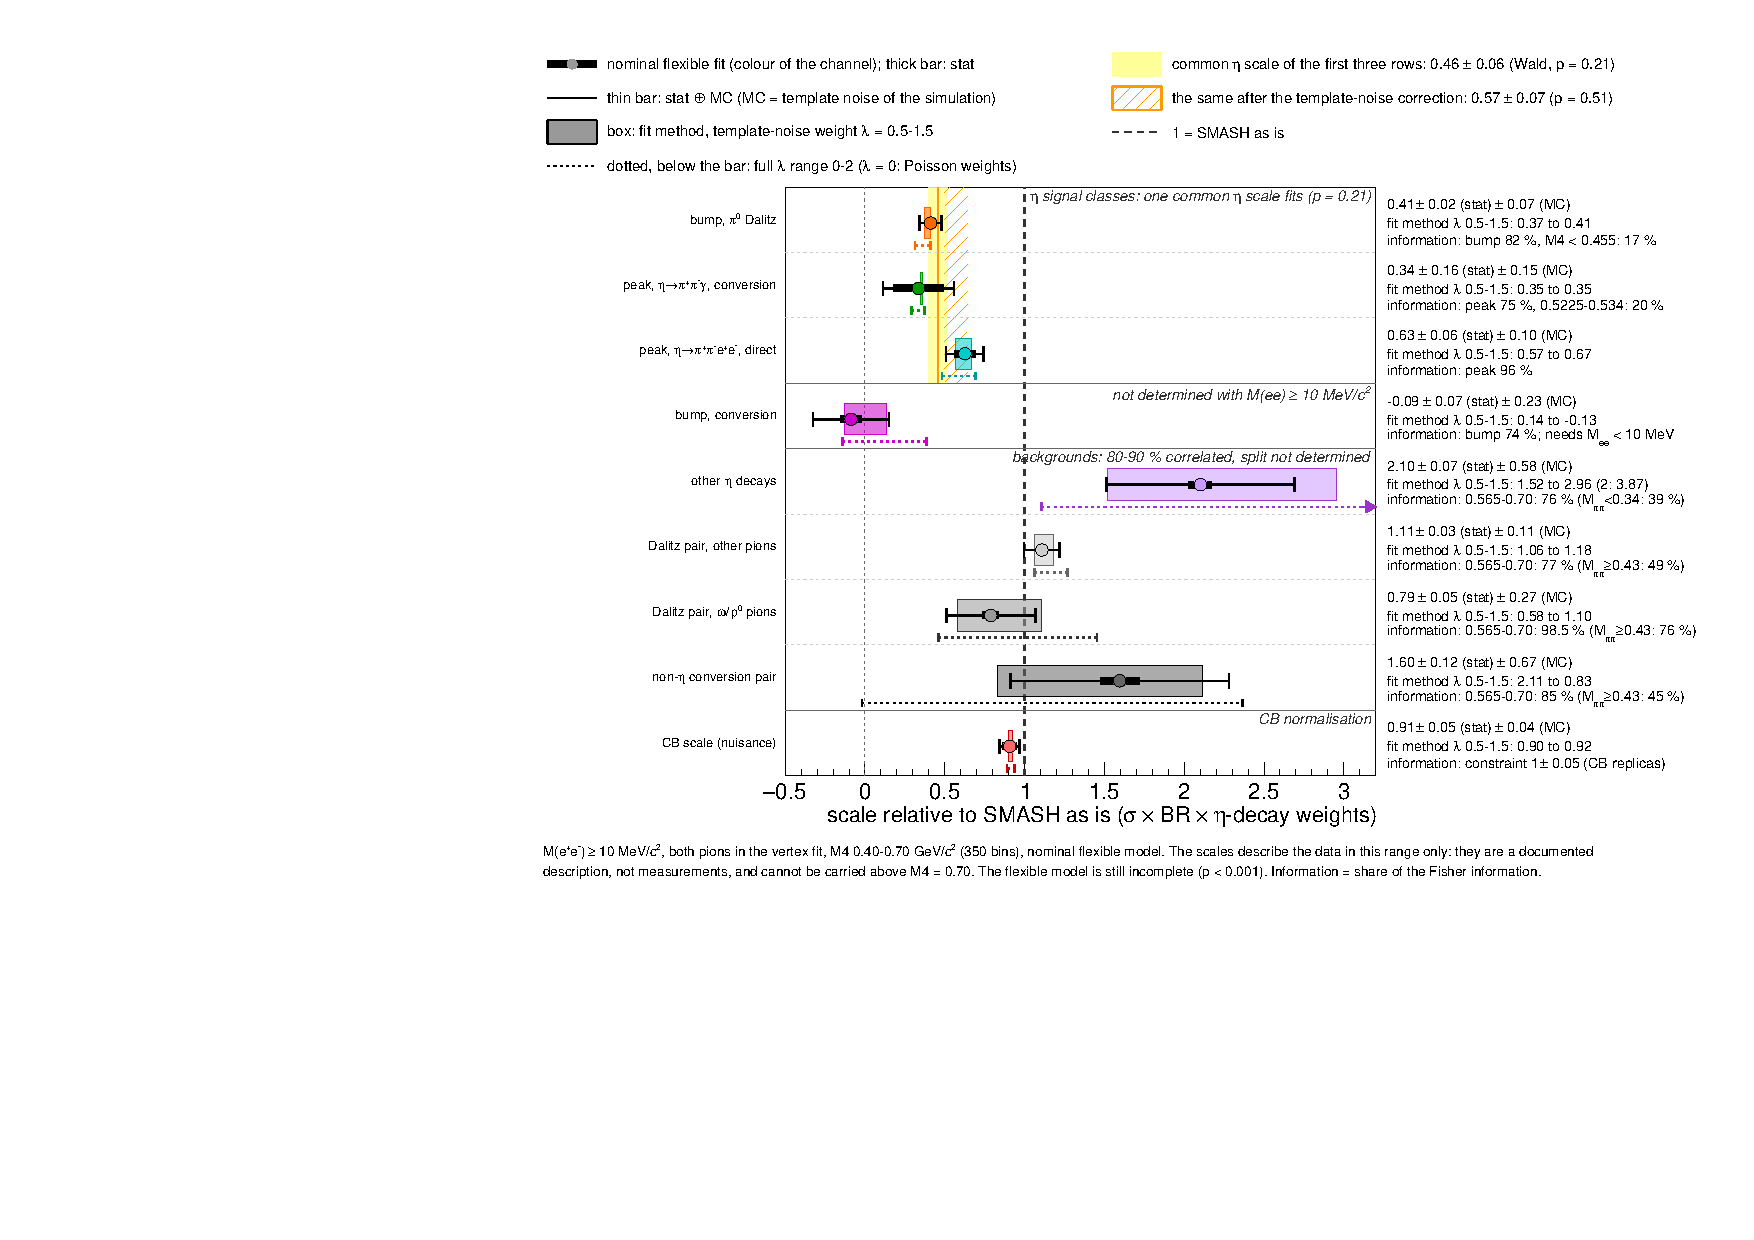
\includegraphics[width=0.94\textwidth]{figs_all/flex_scales_v2_plain.pdf}
\caption{\textbf{What it shows: with a free scale per SMASH channel, the three $\eta$ signal channels (\piz Dalitz bump, peak with converted photon,
direct decays) share one scale of about 0.46 of SMASH; the background scales above the peak are large, correlated and depend on the fit method;
the bump with a converted photon is not determined.} Every scale against 1 (SMASH as it is, dashed), in its channel's colour. Thick bar: stat;
thin: stat $\oplus$ MC. Shaded box: spread with the fit method (weight of the template noise in the fit, 0.5--1.5); dotted line below: weight 0--2 (arrow:
the other $\eta$ decays reach 3.87). Yellow band: the common $\eta$ scale, $0.46\pm0.06$ ($p=0.21$); hatched: $0.57\pm0.07$ after correcting the
downward bias that the template noise causes, as measured on pseudo-data (Table~\ref{tab:freescale}).
Right: value $\pm$ stat $\pm$ MC, the range with the fit method and what fixes the scale (share of the Fisher information from a mass region). A
description, not measurements; not valid above \Mfour$=0.70$\,\GeVcc; model incomplete ($p<0.001$).
\Sel data: \selnom; \Mee$\ge10$\,\MeVcc; \Mfour 0.40--0.70\,\GeVcc in \slicesfive (350 bins); \cbspread, its factor constrained to $1\pm0.05$;
\lumisel. SMASH: \smashsel.
\figlabels{$\lambda$: weight of the template noise in the fit ($\lambda=0$: Poisson weights); Wald: the statistical test of the common
scale; ``information'': the share of the Fisher information from the bump window, the peak window, \Mfour 0.565--0.70 or below 0.455\,\GeVcc,
0.5225--0.534\,\GeVcc and the \Mpipi slices below 0.34 and above 0.43\,\GeVcc.}}
\label{fig:res-freescale}
\end{figure}

%----------------------------------------------------------------------
\subsection{After the typical cuts of earlier analyses}
\inshort{for comparison only: the data still exceed SMASH as it is by 16--45\,\% above the peak; the cuts do not enrich the $\eta$ and make no X17 easier to see.}
Earlier analyses select $\eta$-like combinations with the angle between the \pipi and \ee systems below $50^\circ$ in the laboratory and above
$140^\circ$ in the $\eta$ rest frame and \Mpipi$<0.46$\,\GeVcc (in a tighter variant 0.42\,\GeVcc), often with an \ee opening angle above $2^\circ$; an opening
angle below $6^\circ$ was proposed because X17 pairs are expected to be close. These cuts are not used for any result here. After them SMASH as it is
still lies below the data just above the peak: data/SMASH in 0.56--0.70\,\GeVcc is 1.23--1.45 on the base selection (1.354 after the full set of earlier
cuts) and 1.16--1.34 on the nominal selection (Fig.~\ref{fig:res-typcuts}). With the $\eta$ channels $\times0.40$ and the non-$\eta$ background
$\times$1.25--1.52 SMASH describes the selections built on the nominal one about as well as the nominal one. The cuts do not enrich the $\eta$ (at a
fixed \Mfour the $\eta$-rest angle cannot tell an $\eta$ from a background combination), and they act on a simulated X17 as on the direct decays.
In a simple count the nominal selection alone stays the most sensitive for X17 (an opening angle below $6^\circ$ raises the signal-to-background
ratio by 19\,\% but keeps only 58\,\% of the X17). \emph{Comparison only} (\S\ref{sec:typcuts}).

\begin{figure}[!tbp]
\centering
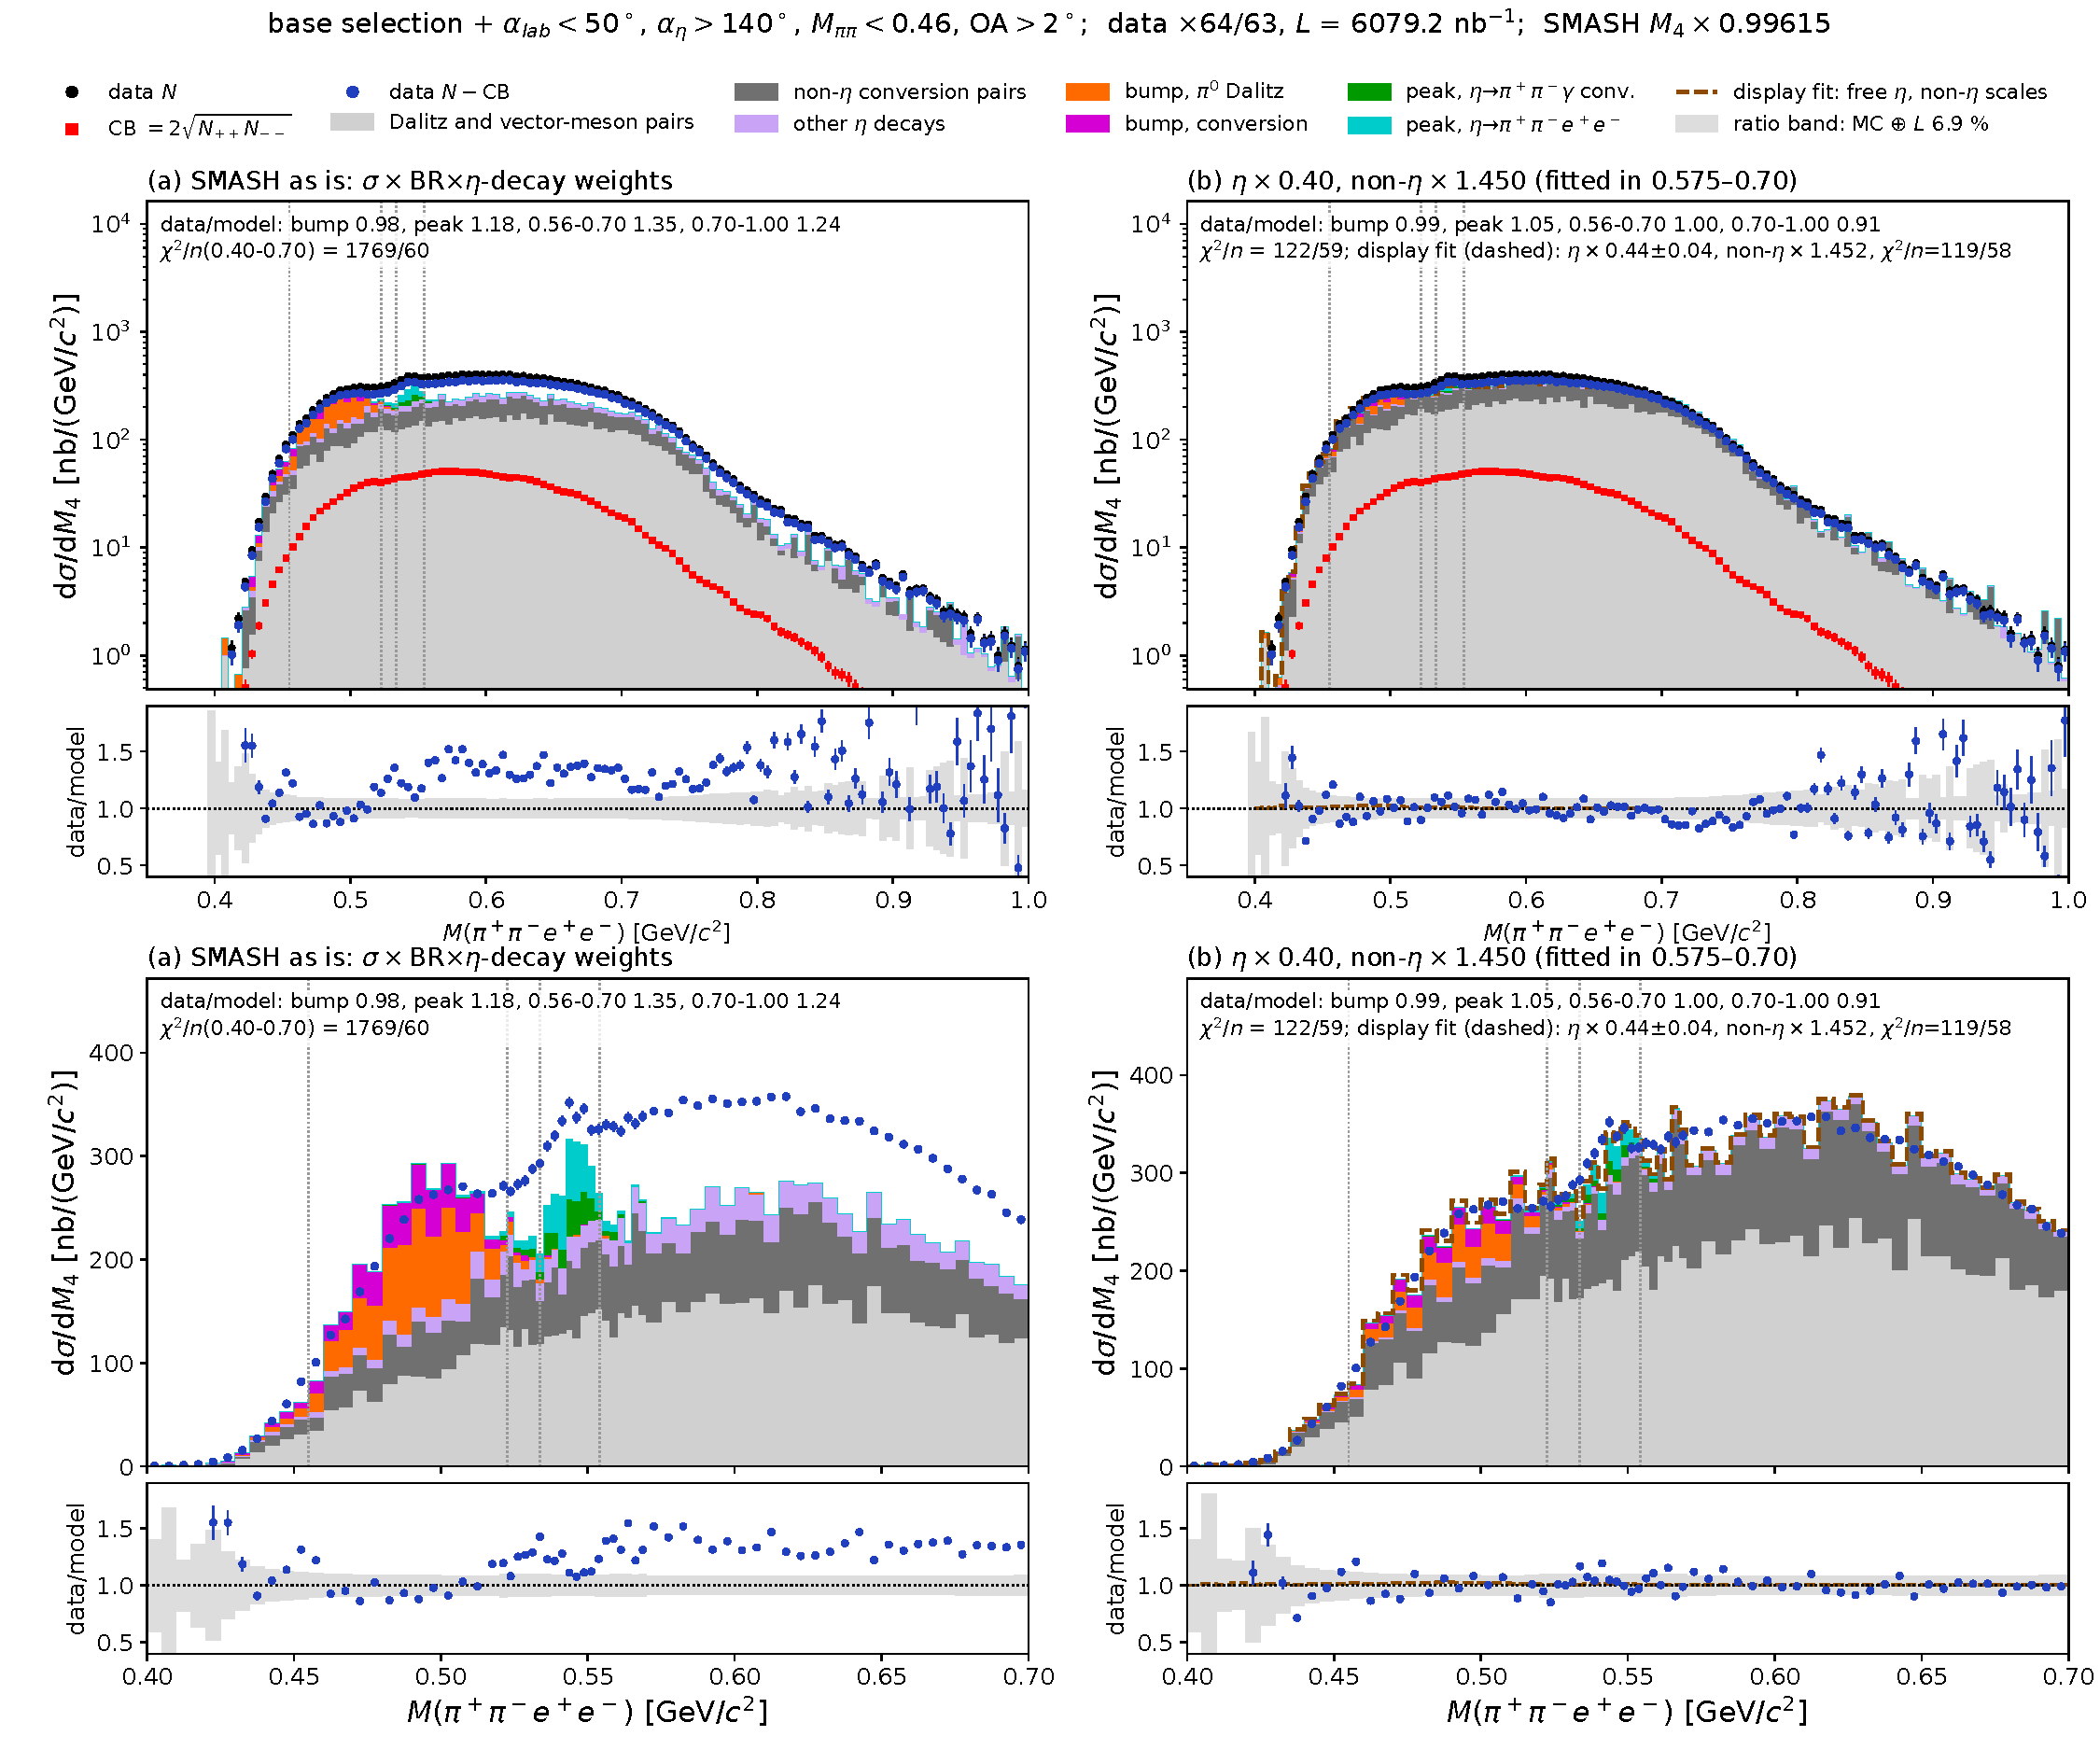
\includegraphics[width=0.90\textwidth]{figs_all/e1_m4_pre_E1_v2_plain.pdf}
\caption{\textbf{What it shows: after the cuts of earlier analyses SMASH as it is still lies below the data above the peak; scaled, it follows
them.} Data: all counts $N$ black, CB red, $N-\mathrm{CB}$ blue, in units of cross section. (a) SMASH as it is, with the data 35\,\% above it at
0.56--0.70\,\GeVcc. (b) Every $\eta$ channel $\times0.40$ and the non-$\eta$ background $\times1.450$ (fitted in 0.575--0.70\,\GeVcc, all \Mee and
\Mpipi); dashed brown: a two-parameter display fit (free $\eta$ and non-$\eta$ scales), not a yield. Stack: background without a conversion pair
light grey, with one dark grey, other $\eta$ decays violet, \piz Dalitz bump orange, converted-photon bump magenta, $\eta\to\pipi\gamma$ with
converted photon green, direct decays cyan. Top: log scale, 0.35--1.00\,\GeVcc; bottom: linear, 0.40--0.70\,\GeVcc; ratio pads: data/model, grey
band SMASH MC $\oplus$ 6.9\,\% of $L$; dotted lines: bump and peak windows.
\Sel data: \selbase (no pion-vertex condition); plus the cuts of earlier analyses: angle between the \pipi and \ee momenta in the laboratory
below $50^\circ$, the same angle in the $\eta$ rest frame above $140^\circ$, \Mpipi below 0.46\,\GeVcc, \ee opening angle above $2^\circ$; \cbsel;
\lumisel. SMASH: \smashsel (the \Mpipi cut on the moved \Mpipi).
\figlabels{$\alpha_{\mathrm{lab}}$, $\alpha_\eta$: the angle between the \pipi and \ee momenta in the laboratory and in the $\eta$ rest frame;
$M_{\pi\pi}$: \Mpipi; OA: \ee opening angle; $\chi^2/n$: $\chi^2$ per degree of freedom.}}
\label{fig:res-typcuts}
\end{figure}

%----------------------------------------------------------------------
\subsection{Discussion: the approach of the earlier analysis}
\label{sec:prevstyle}
\inshort{drawn as in the earlier analysis, SMASH scaled to the data integral gets the total right but the parts wrong; with our measured scales
it describes the data up to 0.70\,\GeVcc; the three-scale fit of the earlier analysis describes the spectrum, but its $\eta$ scales move with
the treatment of the simulated shapes; a demonstration with the background fixed on the slope and two free $\eta$ scales (not a measurement)
gives scales that move with the assumed background shape (0.47 and 0.67\,mb as cross sections; X17 limits of 1.6--$13\times10^{-5}$
from a simple count, depending on choices).}
At the analyst's request the data after the typical cuts are also shown as in the earlier analysis presented at HADES collaboration meetings:
a linear \Mfour spectrum with SMASH scaled to the integral of the data minus CB and the $\eta$ decays drawn as separate lines
(Fig.~\ref{fig:prev-m4}), and a global fit with three free scales (Fig.~\ref{fig:prev-fit}). All stored combinations of each event are the
nominal choice; the best combination only is drawn because the earlier analysis used it, and it gives the same picture. One factor for all
of SMASH (1.245) makes the total right by construction, but the parts are wrong: SMASH is about 20\,\% too high in the bump window
(data/model 0.81) and about 10\,\% too low just above the peak (1.09 in 0.56--0.70\,\GeVcc; $\chi^2/\mathrm{ndf}=5.8$), so this picture
says nothing about the size of the $\eta$ signals. With our measured scales SMASH describes the data up to 0.70\,\GeVcc (data/model 1.00,
1.05 and 1.00 in the bump window, the peak window and just above the peak; $\chi^2/\mathrm{ndf}=2.1$). The three-scale fit gives the $\eta$
peak at 0.65--0.74 of SMASH and the bump at 0.49--0.70, depending on how the simulated shapes are treated (with the background shape
smoothed over a wider mass range the peak even falls to 0.45--0.48): the background (all but the two $\eta$ parts) is 95\,\% of the counts
in the fit range, its simulated shape is wrong at the level of the data errors, and the two small $\eta$ parts absorb that error. Our dedicated measurements,
0.418 (peak) and 0.426 (bump, from its kinematic edge), do not depend on the background level. Both approaches agree that the SMASH $\eta$
must come down by a factor 1.4--2.4 and the non-$\eta$ background go up by 25--45\,\%. In the same style, the \Mee spectrum of the $\eta$
peak window minus the side bands follows the simulated $\eta$ shape, but its small residual in the X17 window changes sign when the
side-band normalisation or the $\eta$ scale is changed within reason, so it cannot test X17. \emph{Discussion, not a measurement}; the full
report gives the fit variants and the \Mee view in its \S4.8 (``The approach of the earlier analysis: integral scaling, a three-scale fit and side bands'').

Fig.~\ref{fig:prev-twoscale} shows, at the analyst's request, the earlier style with the background fixed on the slope right of the $\eta$
peak and two free scales for the $\eta$ bump and the $\eta$ peak. \textbf{This is a demonstration in the style of the earlier analysis. It is
not a measurement and no result of this report uses it.} Under the bump the assumed background is 5.4 times the bump, so the bump scale
($0.455\pm0.049$ of SMASH) moves with the assumed background shape (0.37--0.54 for a tilt of 3\,\% per 0.1\,\GeVcc); this is why we
measure the bump at its kinematic edge, a sharp step that a smooth background cannot make.

Turned into a cross section with the same steps as our results, the two scales of this demonstration give 0.47\,mb from the bump and
0.67\,mb from the peak (uncertainty about 25 and 30\,\%, mostly from the assumed background shape), against 0.444 and 0.429\,mb from our
measurements: in this picture the two $\eta$ signals disagree by a factor 1.4. Counting, as the earlier analysis did, the \ee pairs of the
$\eta$ peak in the X17 mass window after subtracting the side bands and the rest of the $\eta$ peak gives 90\,\% CL upper limits of about
$(5$--$8)\times10^{-5}$ on \BRX, but anywhere between 1.6 and $13\times10^{-5}$ with other reasonable side-band normalisations and $\eta$
scales; our fit of the full \ee mass spectrum gives $3.16\times10^{-5}$, because it measures its background instead of assuming it.
\textbf{This is a demonstration in the style of the earlier analysis. It is not a measurement and no result of this report uses it.}

\begin{figure}[!tbp]
\centering
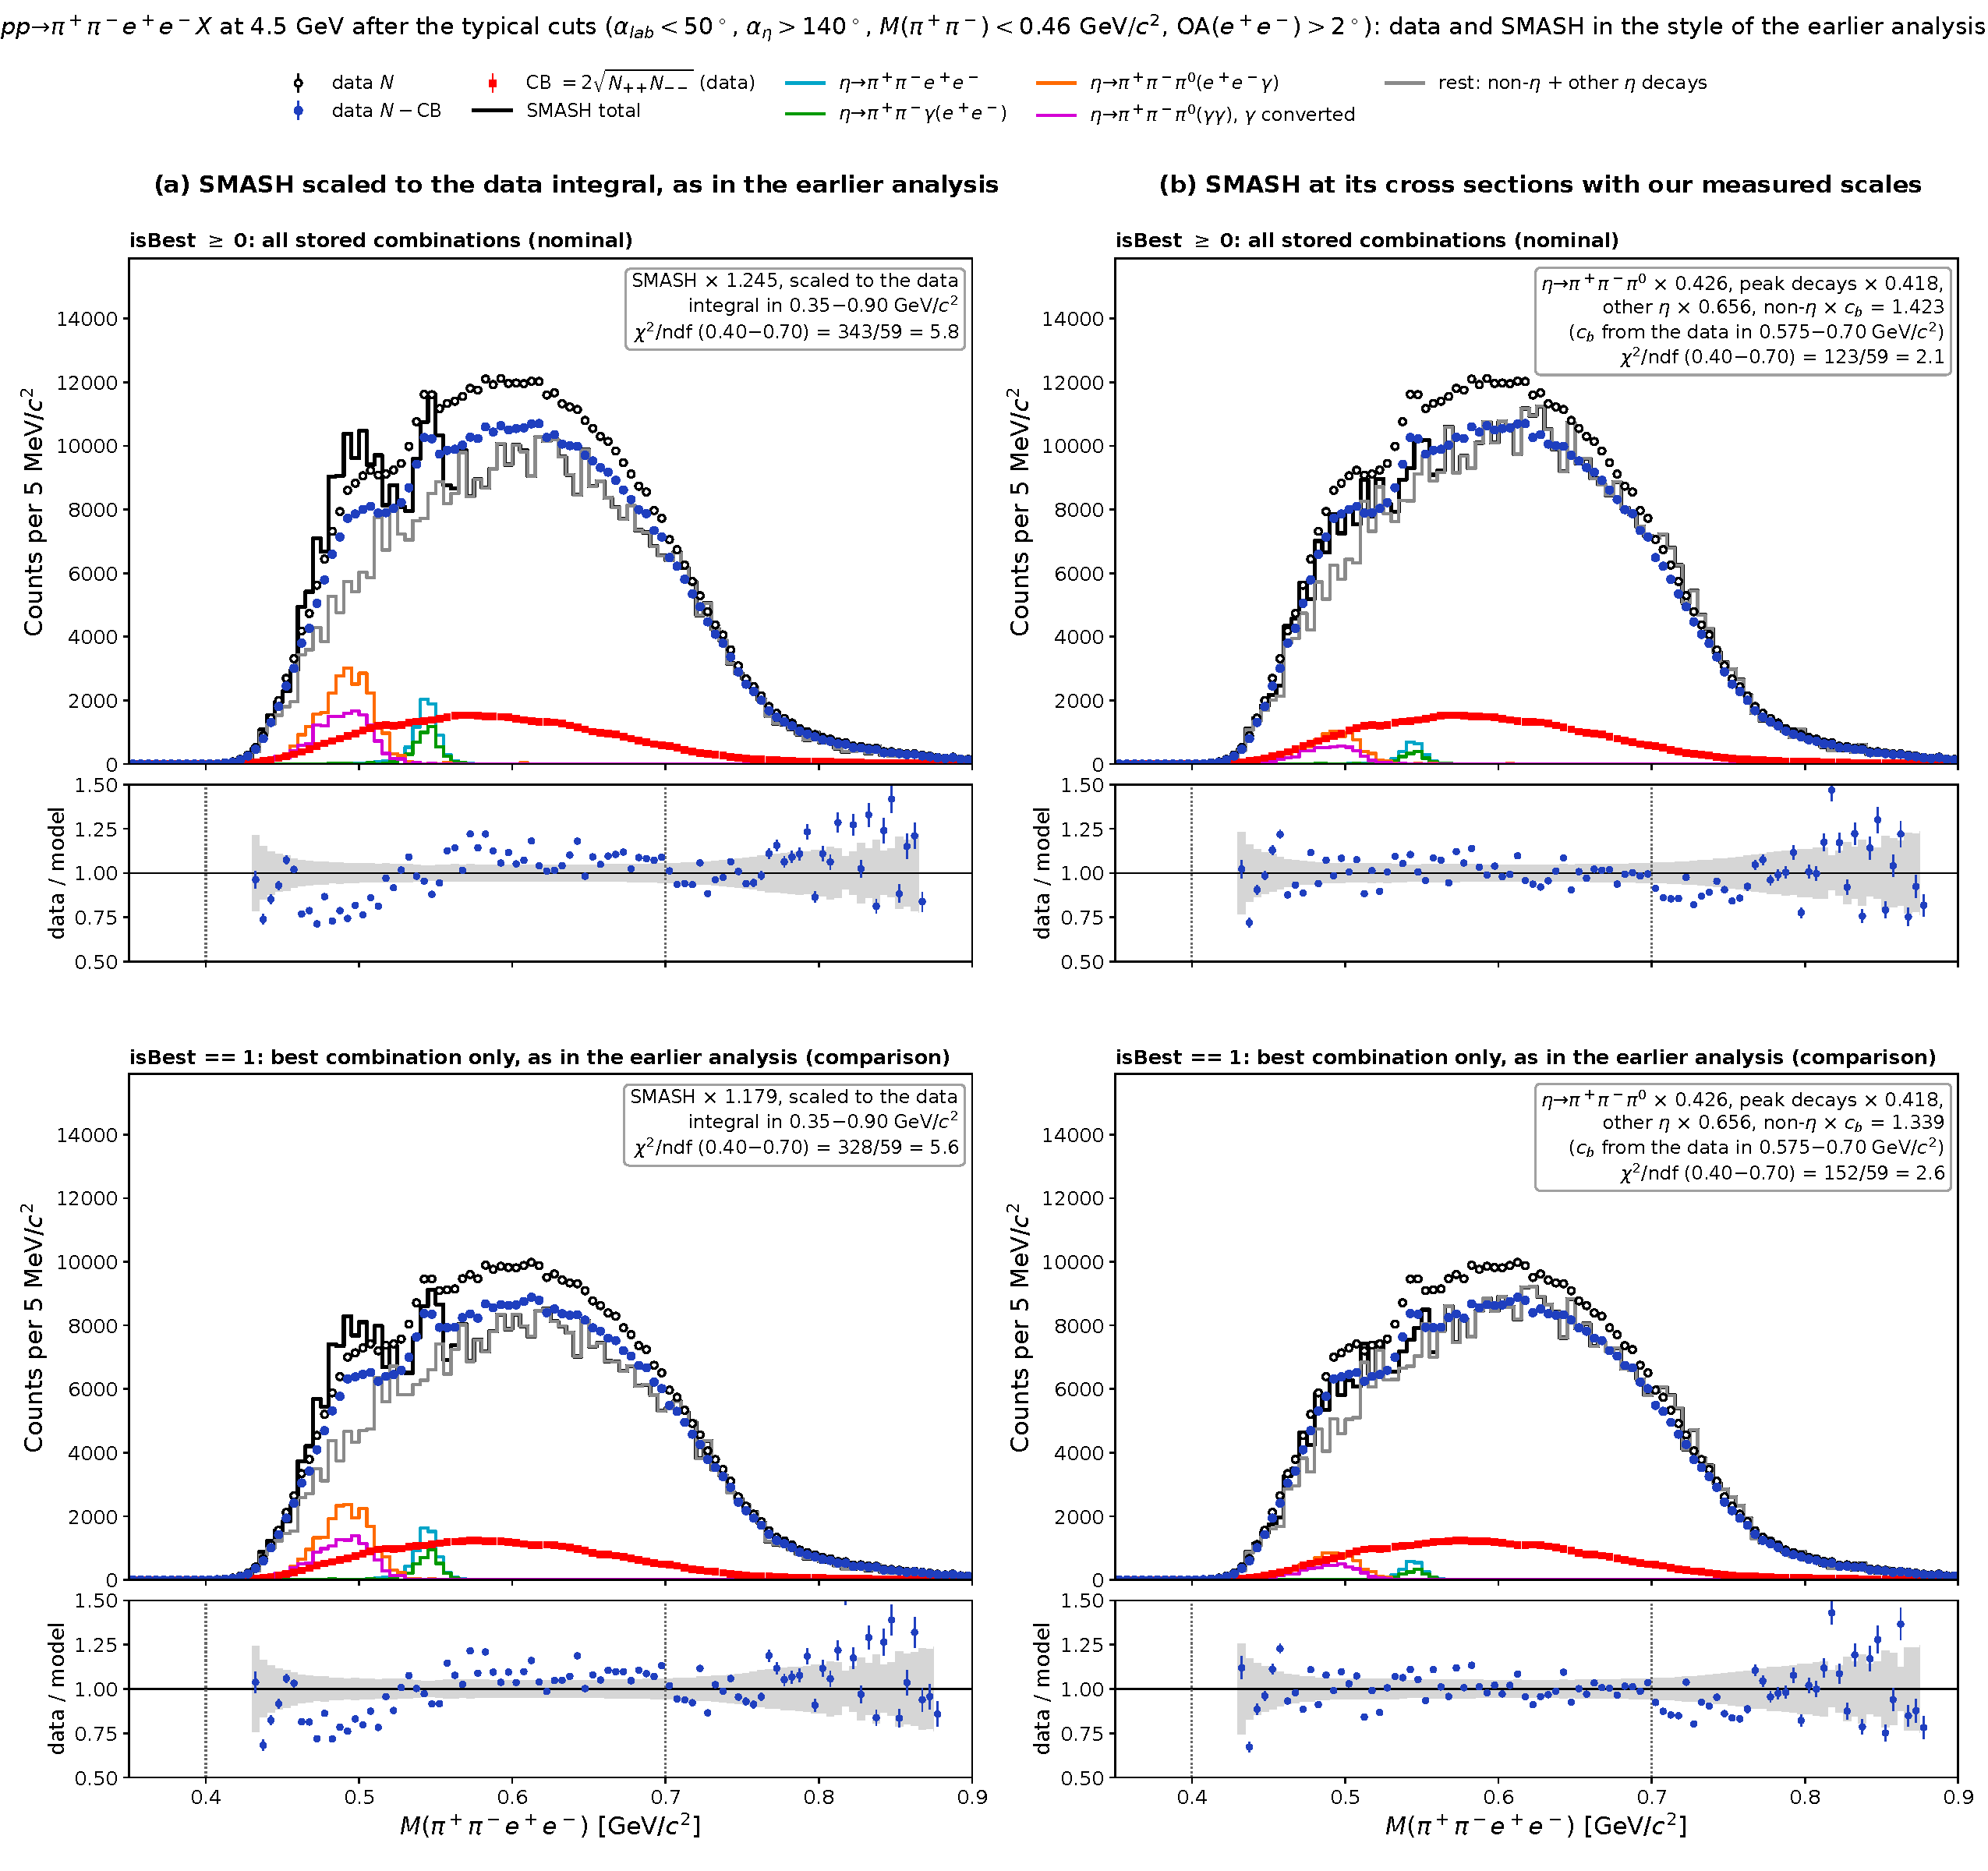
\includegraphics[width=0.74\textwidth]{figs_all/prevstyle_m4_E1.pdf}
\caption{\textbf{What it shows: SMASH scaled to the integral of the data, as in the earlier analysis, gets the total right but the parts wrong:
about 20\,\% too high in the bump and 10\,\% too low just above the peak. With our measured scales it describes the data up to 0.70\,\GeVcc
($\chi^2/\mathrm{ndf}$ 2.1 instead of 5.8).} Linear \Mfour, counts per 5\,\MeVcc. Data: all counts $N$ (open black circles), CB (red),
$N-\mathrm{CB}$ (blue). SMASH: total (black); $\eta\to\ppee$ (cyan); $\eta\to\pipi\gamma$, photon converted (green); $\eta\to\pipi\piz$ with
$\piz\to\gamma\ee$ (orange) or $\piz\to\gamma\gamma$, one photon converted (magenta); rest: non-$\eta$ background and other $\eta$ decays (grey).
(a) All of SMASH $\times$ one factor matching the integral of $N-\mathrm{CB}$ in 0.35--0.90\,\GeVcc (1.245 top, 1.179 bottom).
(b) $\eta\to\pipi\piz$ $\times0.426$ (bump edge), the two peak decays $\times0.418$ (peak), other $\eta$ decays $\times0.656$, non-$\eta$ background
$\times1.423$ (top) or 1.339 (bottom), fitted to the data in 0.575--0.70\,\GeVcc. Lower pads: $(N-\mathrm{CB})$/model; grey band: SMASH
statistics; dotted lines: the $\chi^2$ range 0.40--0.70\,\GeVcc (data and SMASH errors). Top row: all stored combinations of each event
(nominal); bottom row: best combination only (one per event, picked from the timing of its tracks), in data and SMASH, as in the earlier
analysis (comparison only).
\Sel data: \selbase; plus \seltyp; \cbsel (best combination only: from the best like-sign combinations, the simple rule of the earlier
analysis, which tends to overestimate the CB). SMASH: \smashsel (the \Mpipi cut on the moved \Mpipi), the \piz Dalitz decays of the bump
weighted to the QED decay angle, expected counts for $L\times63/64$ (trigger bit), $L=6079.2\,\nbinv$.
\figlabels{isBest $\ge0$ / $==1$: all stored combinations / best combination only; $\alpha_{\mathrm{lab}}$, $\alpha_\eta$: the angle between
the \pipi and \ee momenta in the laboratory and in the $\eta$ rest frame; OA: \ee opening angle; $\gamma(\ee)$: converted photon; $c_b$: the
factor of the non-$\eta$ background; $\chi^2$/ndf: $\chi^2$ per degree of freedom in 0.40--0.70\,\GeVcc.}}
\label{fig:prev-m4}
\end{figure}

\begin{figure}[!tbp]
\centering
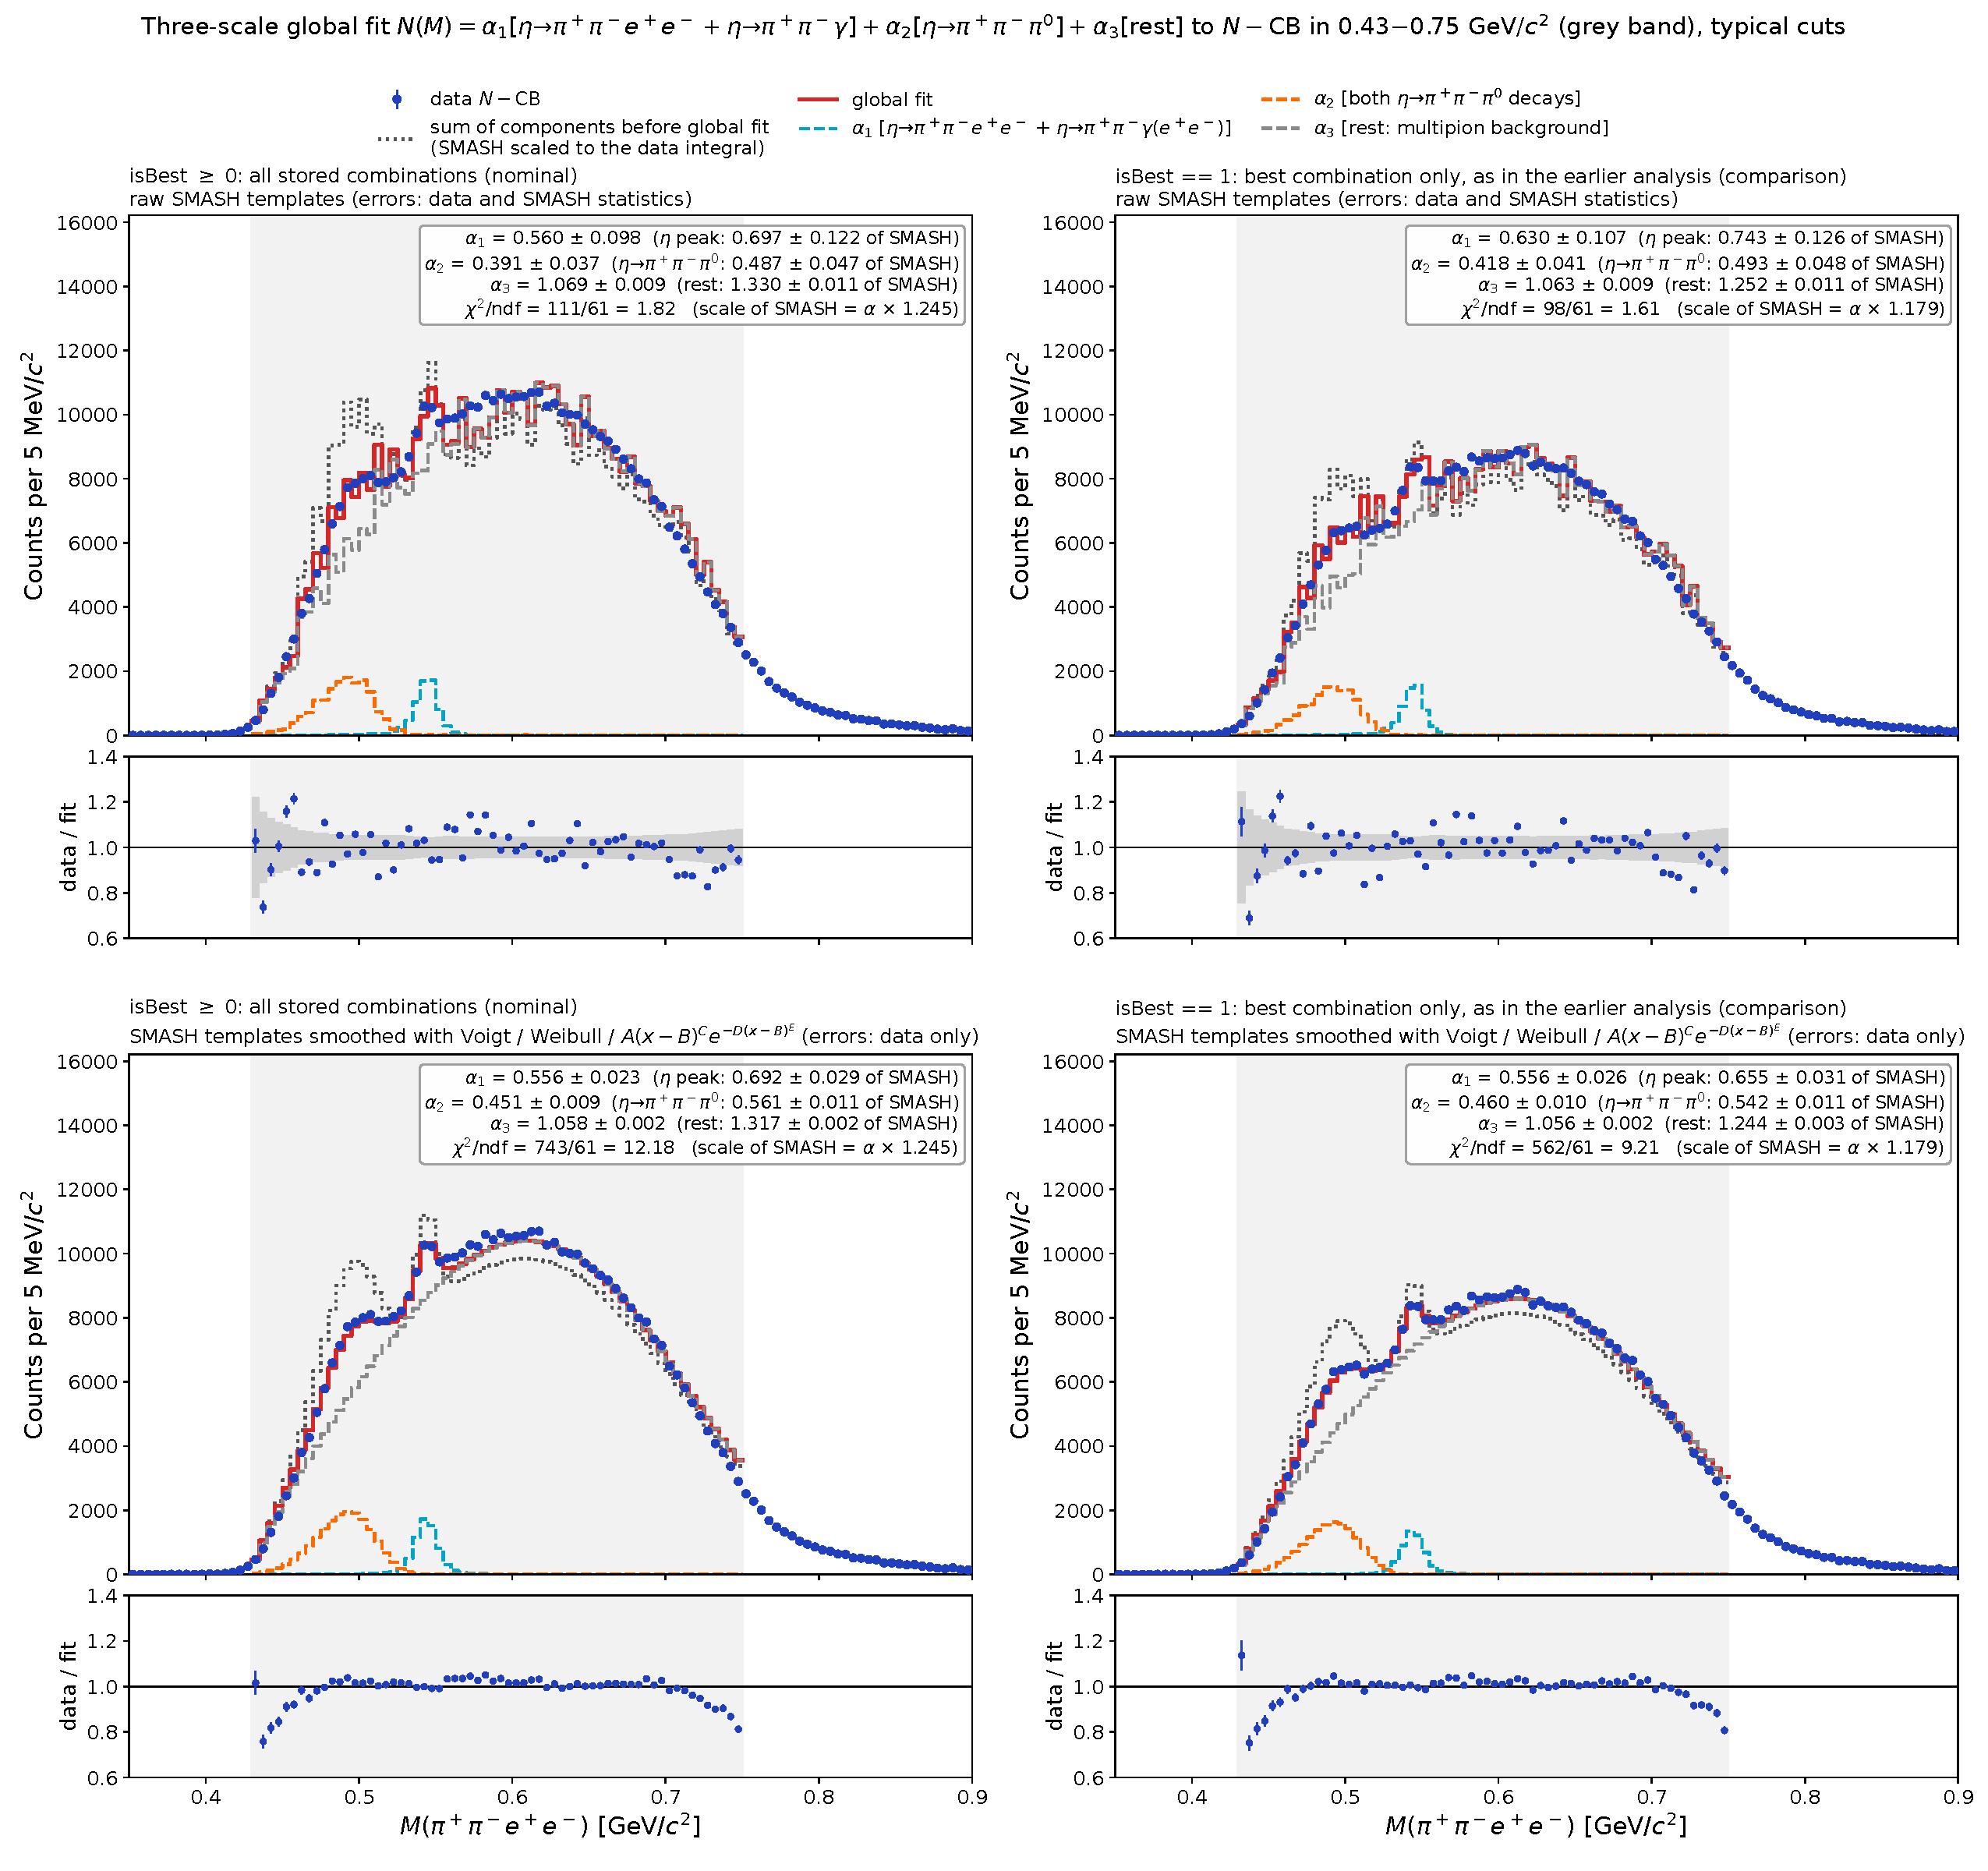
\includegraphics[width=0.74\textwidth]{figs_all/prevstyle_globalfit_E1.pdf}
\caption{\textbf{What it shows: the three-scale global fit of the earlier analysis describes the spectrum, but its $\eta$ scales depend on how
the simulated shapes are treated: for all stored combinations the $\eta$ peak comes out at 0.69--0.70 of SMASH and the bump decays at
0.49--0.56, against 0.418 and 0.426 from our dedicated measurements. The scales are a display, not yields.} Fit of $N-\mathrm{CB}$ (blue) in
0.43--0.75\,\GeVcc (grey band, 5\,\MeVcc bins) with three free factors: $\alpha_1$ for the $\eta$ peak ($\eta\to\ppee$ and $\eta\to\pipi\gamma$,
photon converted; cyan dashed), $\alpha_2$ for both $\eta\to\pipi\piz$ decays of the bump (orange dashed), $\alpha_3$ for all other SMASH pairs
(grey dashed); red: the fit; dotted: the parts before the fit, SMASH scaled to the data integral as in the earlier analysis.
Box: the factors, the scales relative to SMASH ($\alpha\times$ the integral factor 1.245 or 1.179), $\chi^2/\mathrm{ndf}$. Top: the simulated
spectra as they are (errors: data and SMASH statistics). Bottom: the simulated spectra replaced by fitted smooth functions (errors: data only).
Left: all stored combinations (nominal); right: best combination only (as in the earlier analysis; comparison only). Lower pads: data/fit.
The rest is 95\,\% of the fitted counts and its simulated shape is wrong at the level of the data errors ($\chi^2/\mathrm{ndf}$
9--12 with smooth shapes; data/fit 0.75--0.9 at both ends); the small $\eta$ parts absorb this.
\Sel data: \selbase; plus \seltyp; \cbsel (best combination only: from the best like-sign combinations, as in the earlier analysis).
SMASH: \smashsel (the \Mpipi cut on the moved \Mpipi), the \piz Dalitz decays of the bump weighted to the QED decay angle, expected counts
for $L\times63/64$ (trigger bit), $L=6079.2\,\nbinv$.
\figlabels{isBest $\ge0$ / $==1$: all stored combinations / best combination only; $N(M)$: fitted counts at \Mfour$=M$; $\gamma(\ee)$:
converted photon; rest, multipion background: all SMASH pairs other than the two $\eta$ parts; Voigt, Weibull, $A(x-B)^C e^{-D(x-B)^E}$: the
smooth functions fitted to the simulated peak, bump and rest (the rest in 0.43--0.75\,\GeVcc).}}
\label{fig:prev-fit}
\end{figure}

\begin{figure}[!tbp]
\centering
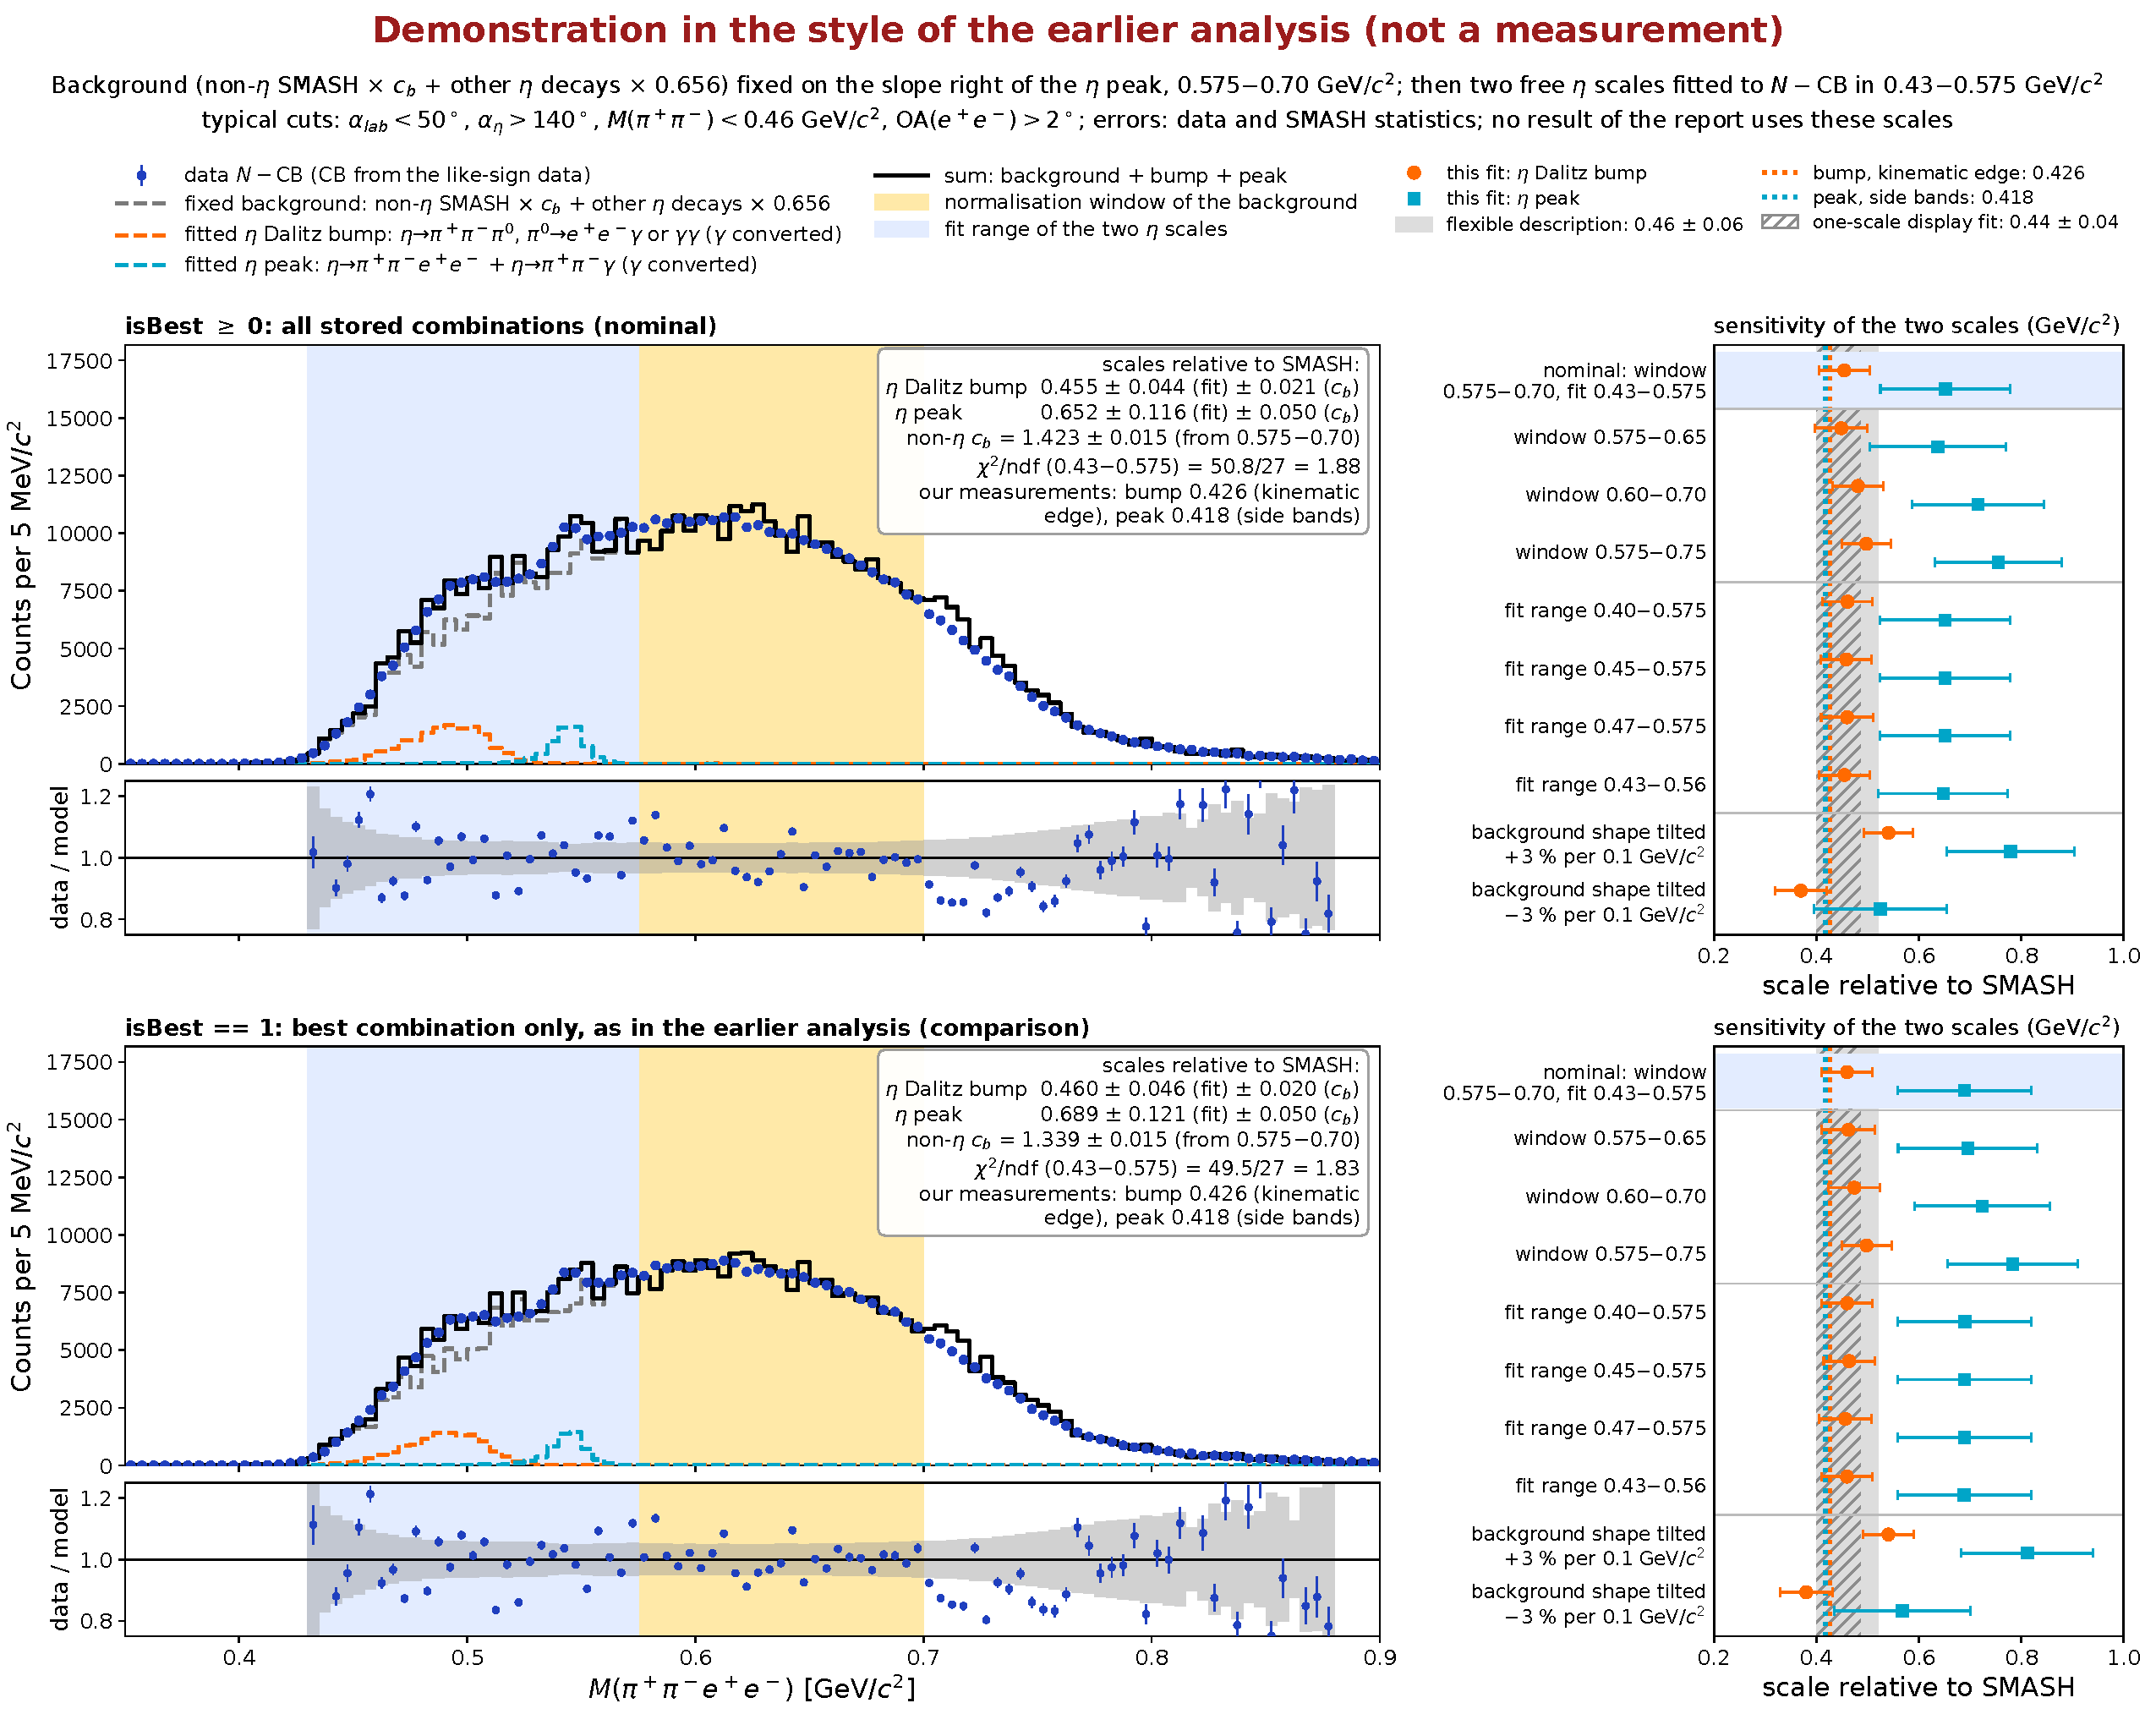
\includegraphics[width=0.70\textwidth]{figs_all/prevstyle_twoscale_E1.pdf}
\caption{\textbf{What it shows: with the background fixed on the slope right of the $\eta$ peak, two free scales put the $\eta$ bump at
0.455 and the $\eta$ peak at 0.65 of SMASH, but both move with the assumed background shape. This is a demonstration in the style of the
earlier analysis. It is not a measurement and no result of this report uses it.}
\Sel data: \selbase; plus \seltyp; \cbsel (best combination only: from the best like-sign combinations, as in the earlier analysis).
SMASH: \smashsel (the \Mpipi cut on the moved \Mpipi), the \piz Dalitz decays of the bump weighted to the QED decay angle, expected counts
for $L\times63/64$ (trigger bit), $L=6079.2\,\nbinv$.
Left: data $N-\mathrm{CB}$ (blue), counts per 5\,\MeVcc. Dashed grey: the fixed background, SMASH pairs not from an $\eta$ $\times1.423$ (top)
or $\times1.339$ (bottom), set so that the model matches the data in 0.575--0.70\,\GeVcc (yellow), plus the other $\eta$ decays $\times0.656$.
Dashed orange: the $\eta$ bump, $\eta\to\pipi\piz$ with the \piz Dalitz decay or with $\piz\to\gamma\gamma$ and one photon converted; dashed
cyan: the $\eta$ peak, $\eta\to\ppee$ and $\eta\to\pipi\gamma$ with the photon converted; each $\times$ its scale fitted to the data in
0.43--0.575\,\GeVcc (light blue; errors of the data and of the SMASH statistics); black: the sum. Lower pads: data/model; grey band:
SMASH statistics. Right: the two scales when the normalisation
window, the fit range or the slope of the background shape is changed, against our measurements: bump 0.426 from its kinematic edge, peak
0.418 from the side bands, $0.46\pm0.06$ from the flexible description and $0.44\pm0.04$ from a one-scale fit after the same cuts. Top row:
all stored combinations of each event (nominal); bottom row: best combination only (as in the earlier analysis; comparison only).
Not to over-read: under the bump the fixed background is 5.4 times the bump and nothing measures it there, so the agreement of the bump scale
with 0.426 is no test; the peak scale follows a few-per-cent mismatch of the simulated background shape around the peak.
\figlabels{isBest $\ge0$ / $==1$: all stored combinations / best combination only; $c_b$: the factor of the background not from an $\eta$;
(fit), ($c_b$): the error of the fit and the error from $c_b$; $\chi^2$/ndf: $\chi^2$ per degree of freedom in the fit range; window:
normalisation window of the background; tilted: the background shape multiplied by a straight line; $\alpha_{\mathrm{lab}}$, $\alpha_\eta$:
the angle between the \pipi and \ee momenta in the laboratory and in the $\eta$ rest frame; OA: \ee opening angle; $\gamma$ converted:
photon converted to an \ee pair.}}
\label{fig:prev-twoscale}
\end{figure}

%----------------------------------------------------------------------
\subsection{Checks that came out fine}
\inshort{the requirement of an event vertex keeps the $\eta$; the target walls carry only $3^{+4}_{-3}$\,\% of the $\eta$ signal.}
The requirement of a reconstructed event vertex keeps $0.994\pm0.021$ of the $\eta$ (SMASH 0.9997); it is not the cause of the low \sigeta (0.93\,mb would need
0.46; Fig.~\ref{fig:vtx}, \S\ref{sec:phys}). The target walls carry only $3^{+4}_{-3}$\,\% of the $\eta$ signal, and the $\eta$ yields are
multiplied by 0.97 for it, although the walls give 13--15\,\% of all counts (Fig.~\ref{fig:res-wallss}); the small $\eta$ share is measured
(Fig.~\ref{fig:res-fetas}: the $\eta$ per count falls to about zero where the walls dominate, and the $\eta$ are distributed along the cell as in
the liquid-hydrogen simulation). \emph{Measured.}

\begin{figure}[!tbp]
\centering
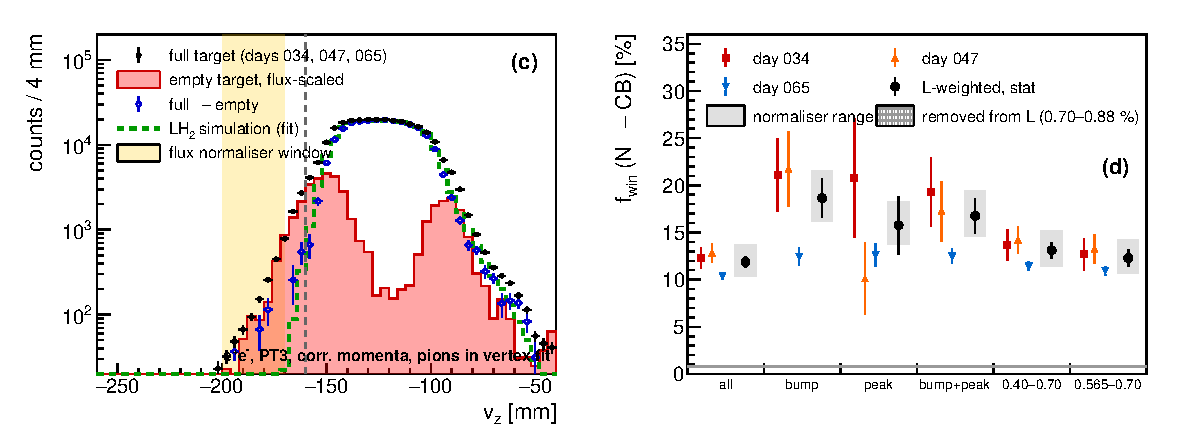
\includegraphics[width=0.84\textwidth]{figs_all/wp2_N1v2_cnt_plain_crop3.pdf}
\caption{\textbf{What it shows: the target walls give 13--15\,\% of the data minus CB, which SMASH does not simulate.} Two panels, (c) and (d), of
a larger figure. (c) Vertex $z$ of the unlike-sign counts on days 034, 047 and 065: full target (black), empty target scaled by the flux ratio of
the same day (red; flux ratio from the counts at $-200$ to $-170$\,mm, shaded), their difference (blue), liquid-hydrogen simulation fitted to the
full-target profile (green). (d) The material share of the data minus CB per \Mfour window, per empty-target day and luminosity-weighted
(statistical errors; grey boxes: range of the flux ratio; hatched: the elastic-window share already removed from $L$, 0.70--0.88\,\%);
0.40--0.70\,\GeVcc: $13.1\pm0.9$\,\%. This is the share of all counts, mostly non-$\eta$ background; the share of the $\eta$ signal is
$3^{+4}_{-3}$\,\% (Fig.~\ref{fig:res-fetas}).
\Sel (c): \selnovtx; a reconstructed event vertex with both pions used in its fit, no cut on the vertex position (the dashed line marks
$\vz>-160$\,mm); all \Mfour. (d): \selnom; data minus CB with \cbsel; the \Mfour windows: all, bump 0.4550--0.5225, peak 0.53364--0.55416, bump
and peak, 0.40--0.70 and 0.565--0.70\,\GeVcc.
\figlabels{$f_{\mathrm{win}}$: the material share of the counts; LH$_2$: liquid hydrogen; L-weighted: luminosity-weighted.}}
\label{fig:res-wallss}
\end{figure}

\begin{figure}[!tbp]
\centering
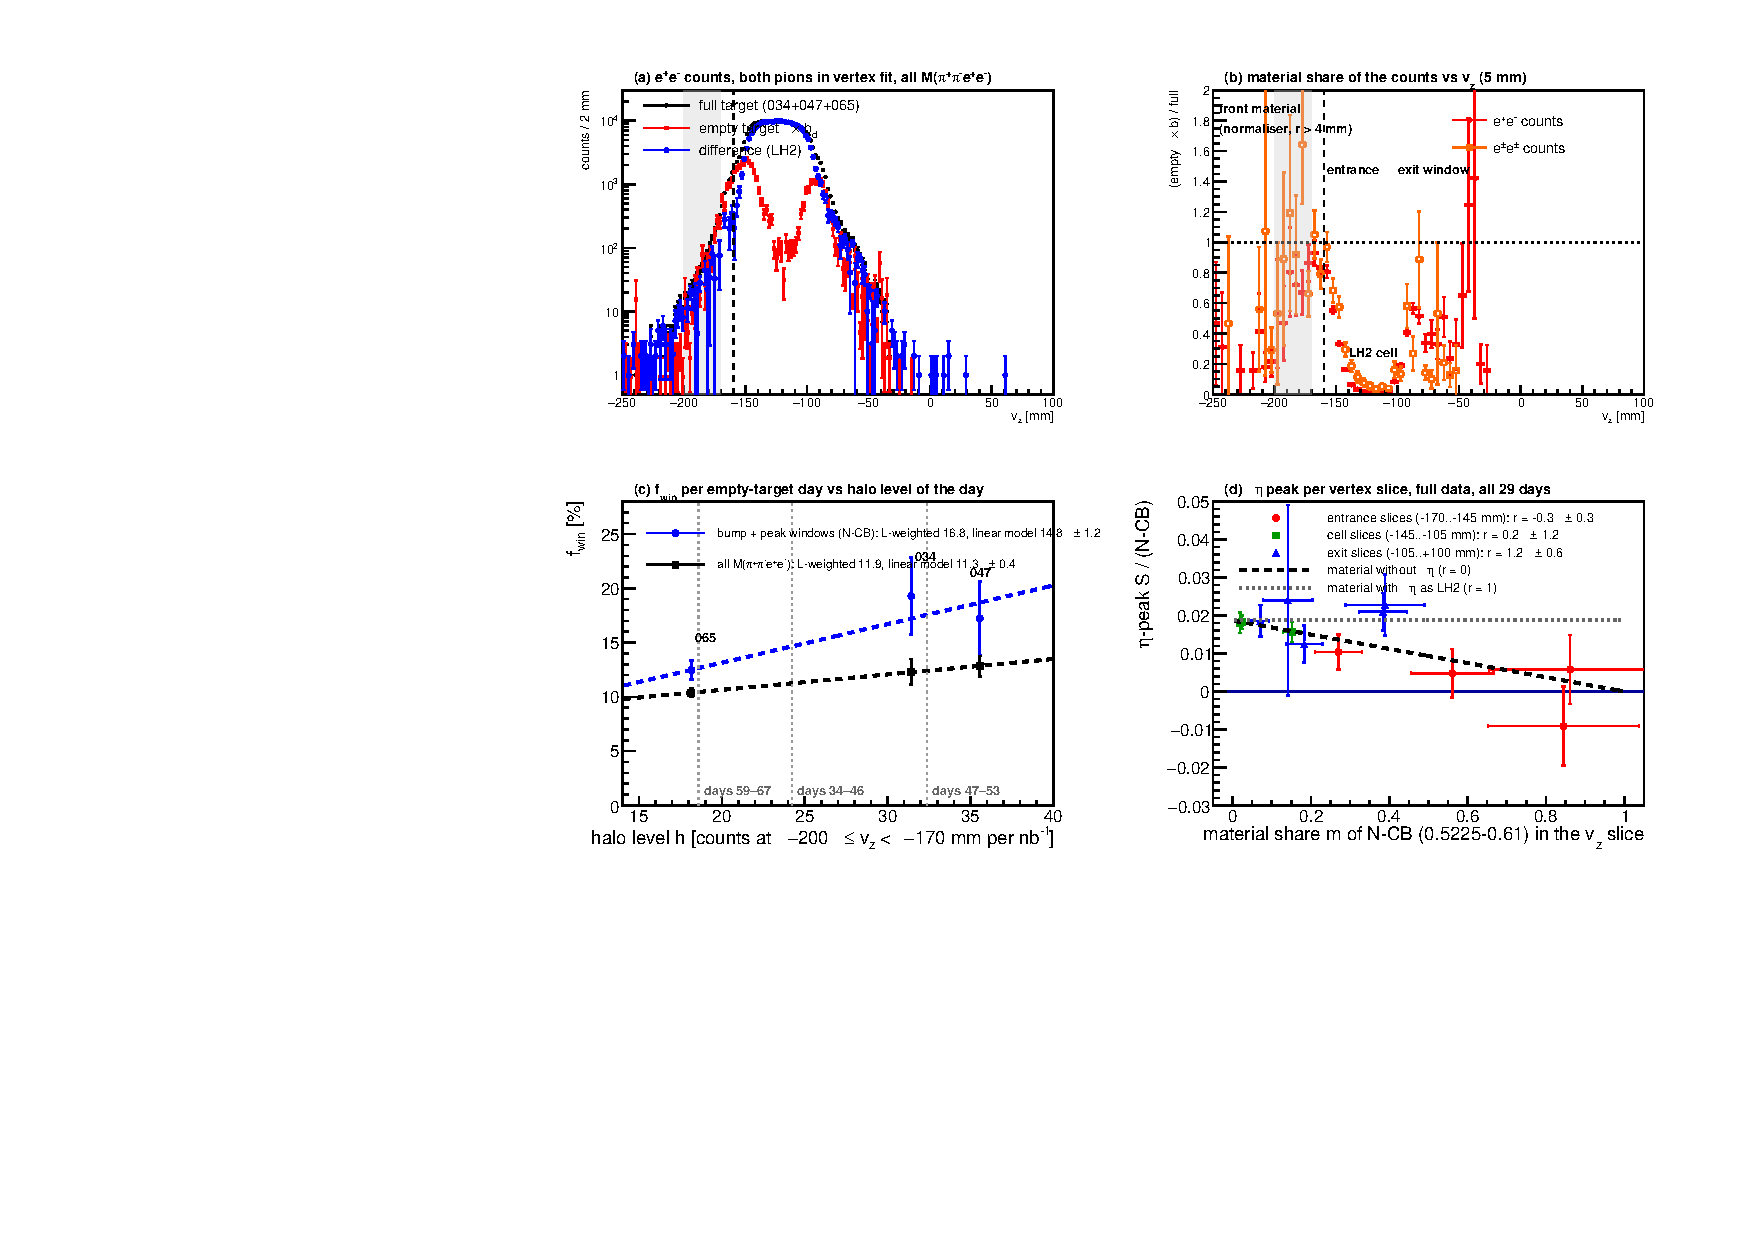
\includegraphics[width=0.92\textwidth]{figs_all/vw2a_fig_cnt_plain.pdf}
\caption{\textbf{What it shows: almost none of the $\eta$ signal comes from the target walls ($3^{+4}_{-3}$\,\%), so the $\eta$ yields are
corrected by 0.97 only, not by the wall share of all counts.} (a) Vertex $z$ of the \ee counts, days 034\,+\,047\,+\,065: full target (black),
empty target scaled by the flux ratio of the same day (red), their difference (blue). (b) Material share of the counts per 5\,mm slice of $\vz$:
the walls dominate at the entrance window ($\approx-150$\,mm) and the exit window ($\approx-90$\,mm); inside the liquid-hydrogen cell they give
about 1\,\%. (c) Material share per empty-target day against the beam-halo level of that day (counts per luminosity with the vertex 170--200\,mm
upstream; dotted lines: the halo levels of the beam periods): it follows the halo, and the empty-target days had a high halo; reweighted to the
luminosity-weighted halo, the share in the bump and peak windows is $14.7\pm1.1$\,\% instead of 16.8\,\%. (d) The decisive test, on the full
data of all 29 days: the $\eta$-peak content per data-minus-CB count in each $\vz$ slice against the material share of that slice. If the walls
produced no $\eta$, the points would follow the dashed line (falling to zero at material share 1); if they produced $\eta$ like hydrogen, the
dotted line. The entrance-window slices (red), where the walls give 30--90\,\% of the counts, fall to about zero: the fitted ratio of $\eta$ per
count in the material to that in hydrogen is $0.07\pm0.30$, i.e.\ a material share of the $\eta$ signal of $3^{+4}_{-3}$\,\% (1--8\,\% over the
vertex models). The exit-window slices (blue) alone give $1.2\pm0.6$ (legend); the walls make a smaller share of the counts there and the error
is twice that of the entrance slices ($-0.3\pm0.3$), so they constrain the ratio less. An independent check agrees: the share of the $\eta$ peak
and of the ECAL-tagged $\eta$ in the cell centre, $0.566\pm0.045$ and $0.571\pm0.024$, equals the hydrogen simulation (0.577), whereas an $\eta$
material share of 16.8\,\% would give 0.497 (excluded at $3.4\sigma$).
\Sel \selnovtx; a reconstructed event vertex with both pions used in its fit, no cut on the vertex position; (a), (b) all \Mfour; (c) in
addition $\vz>-160$\,mm, bump and peak windows together (0.4550--0.5225 and 0.53364--0.55416\,\GeVcc); (d) 12 slices of $\vz$ from $-170$ to
$+100$\,mm, grouped as entrance ($-170$ to $-145$\,mm), cell ($-145$ to $-105$\,mm) and exit ($-105$ to $+100$\,mm), $\eta$-peak content from a
fixed Gaussian (0.5439\,\GeVcc, 5.4\,\MeVcc) plus a second-order polynomial in \Mfour 0.5225--0.61\,\GeVcc of each slice; CB from the like-sign
counts with the same cuts.
\figlabels{$f_{\mathrm{win}}$: the material share of the counts; L-weighted: luminosity-weighted; LH$_2$: liquid hydrogen; front material: the material in front of the
cell (the flux normaliser); $S$: $\eta$-peak content; $m$: material share of a slice; $r$: the ratio of $\eta$ per count in the material to that
in hydrogen, per group of slices.}}
\label{fig:res-fetas}
\end{figure}

%----------------------------------------------------------------------
\subsection{A defect of the simulation}
\inshort{HGeant decays the virtual photon of \piz Dalitz decays isotropically; the simulated bump efficiency is about 16\,\% too high; the bump-edge values are corrected.}
HGeant (standard SMASH set) decays the virtual photon of $\piz\to\gamma\ee$ isotropically instead of $1+\cos^2\theta^*$: for the bump counts of this
analysis the simulated efficiency is about 16\,\% too high (QED weights per count of the full simulation give 0.86 at the bump edges; toys and the
closure of prompt \piz Dalitz pairs gave 12--14\,\%). It is corrected only in the bump-edge values, count by count: 0.390 $\to$ 0.426 in $u$ and
0.392 $\to$ 0.423 per slice; the peak does not contain these decays (\S\ref{sec:phys}, Fig.~\ref{fig:res-qed}).

\begin{figure}[!tp]
\centering
\begin{minipage}[c]{0.33\textwidth}
\includegraphics[width=\textwidth]{figs_all/wp8_P1_plain_e600.png}
\end{minipage}\hfill
\begin{minipage}[c]{0.64\textwidth}
\caption{\textbf{What it shows: the PLUTO generator decays the virtual photon of $\piz\to\gamma\ee$ as QED predicts, $1+\cos^2\theta^*$; HGeant,
which decays it again in the simulation, uses a flat (isotropic) distribution.} One panel, (e), of a larger figure. Decay angle of
$\piz\to\gamma\ee$ ($e^+$ against the virtual-photon direction, in its rest frame): PLUTO (black: \Mee$<10$\,\MeVcc, blue: \Mee$\ge20$\,\MeVcc)
follows QED (red line); the flat green line is the isotropic distribution of the HGeant decay routine, drawn as a reference (no HGeant output
is plotted). In toys and in the closure of prompt \piz Dalitz pairs the simulated efficiency of these decays is 12--14\,\% too high
(QED/isotropic 0.875--0.891); for the bump counts of this analysis the QED weights per count give 0.86, i.e.\ about 16\,\%.
\Sel generator level, no cuts (PLUTO decays of the lepton simulation set, normalised distributions).}
\label{fig:res-qed}
\end{minipage}
\end{figure}

%----------------------------------------------------------------------
\subsection{What is not determined, and a possible explanation}
\label{sec:notdet}
\textbf{Not determined}: the background-subtracted bump area and the double ratio derived from it (Figs.~\ref{fig:res-peaks}a, \ref{fig:res-afters};
the bump itself is measured through its edge); BR$(\eta\to\ppee)$ (the template fit gives $2.67\times10^{-4}$, consistent with PDG 2026,
$2.76\pm0.16$, but the template fits failed the pseudo-data test and the total uncertainty is about 130\,\%; Fig.~\ref{fig:eta-summary}b); the make-up of the
$\eta$ peak (\sigeta between 0.25 and 0.52\,mb; neither bump edge decides it: the share of converted photons is $0.83\pm0.20\pm0.34$ of SMASH in $u$,
$0.47\pm0.24\pm0.46$ per slice); the split of the non-$\eta$ background and the per-channel SMASH scales as measurements; the significance of the
difference to the HADES values at 3.5\,GeV; the ECAL full reconstruction (feasibility only).

\textbf{A possible explanation, to be tested in a separate analysis.} The data may lose close \ee pairs (small opening angle, small \Mee) more
often than the simulation; then the direct decays (scale 0.50, against 0.24 from the converted photons; Fig.~\ref{fig:eta-summary}a) would give the most
reliable $\eta$ scale, \sigeta $\approx0.52\pm0.06\,(\mathrm{stat})$\,mb. The evidence is suggestive, not conclusive; no number is changed. The test,
outside these reports, measures the reconstruction efficiency of \ee pairs with an opening angle of 0--6$^\circ$ in data and simulation, from \piz,
$\eta$ and $\omega$ Dalitz decays with the \ee pair plus the ECAL photon, once the trigger-bias correction and the new ECAL calibration are ready.

\bigskip
\noindent{\large\bfseries Supporting results}\par
\smallskip
\noindent Sections~\ref{sec:before}--\ref{sec:x17} give the supporting tables and figures; each starts with a one-line summary.

%======================================================================
\section{SMASH against the data before any normalisation}
\label{sec:before}
%======================================================================
\inshort{without any adjustment, data/SMASH depends on \Mfour (from 0.74 to 1.27): 0.86 in the bump window, 1.10 in the peak window, 1.27 just
above the peak and 0.74 at 0.9--1.1\,\GeVcc; one common scale gives $\chi^2$/ndf $=12$.}
Counting true pairs with a ghost track (a track that the simulation flags as not matching one particle) as physical background raises SMASH by
9--17\,\% and lowers these ratios by 8.5--14.5\,\%; about 13--15\,\% of the data minus CB in 0.40--0.70\,\GeVcc is target material, which SMASH
does not simulate. The requirement of an event vertex keeps 0.565 of the data counts in the peak window; the removed counts are mostly not target events, so the
ratios need no vertex correction at the 1\,\% level. The data hold about 0.3 of the SMASH K$^0_S$ (data/SMASH $0.29\pm0.04$); whether this is
SMASH or the vertex selections acting on the displaced pions is not established (the vertex requirement keeps 0.72--0.85 of the data K$^0_S$, which
explains at most a factor 1.4). The K$^0_S$ position confirms the \Mpipi scale. Table~\ref{tab:before} lists the ratios per region for the
nominal and the base selection; Fig.~\ref{fig:zoom} shows the region around the $\eta$ in linear scale.

\begin{figure}[!htbp]
\centering
\begin{minipage}[c]{0.40\textwidth}
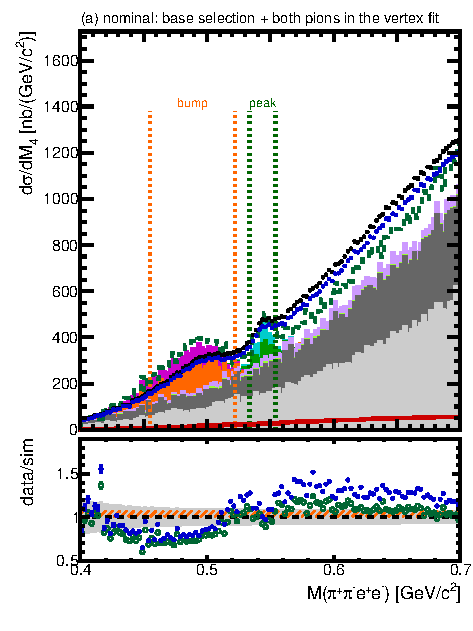
\includegraphics[width=\textwidth]{figs_all/wp1_B2_plain_crop.pdf}
\end{minipage}\hfill
\begin{minipage}[c]{0.57\textwidth}
\centering
\captionof{table}{Data/SMASH before any normalisation (errors data $\oplus$ MC; the 6.9\,\% of $L$ not included). Jump: ratio in 0.560--0.595 over
ratio in 0.4875--0.5225\,\GeVcc; shape: one free scale $a$ in 0.40--0.70\,\GeVcc, 60 bins. Nominal selection; base: the same without the
pion-vertex condition. Data counts $\times64/63$, $L=6079.2\,\nbinv$; CB from the like-sign data; SMASH as stated below the figure.}
\label{tab:before}
\footnotesize
\begin{tabular}{@{}l r r@{}}
\toprule
\Mfour region [\GeVcc] & nominal & base \\
\midrule
bump window 0.4550--0.5225 & $0.861\pm0.013$ & $0.949\pm0.013$ \\
peak window 0.5336--0.5542 & $1.101\pm0.022$ & $1.212\pm0.022$ \\
0.565--0.70 & $1.266\pm0.008$ & $1.350\pm0.008$ \\
0.90--1.10 & $0.744\pm0.003$ & $0.784\pm0.003$ \\
jump & $1.467\pm0.036$ & $1.431\pm0.032$ \\
shape $\chi^2$/ndf & 723.7/59 & 765.1/59 \\
free scale $a$ & 1.191 & 1.279 \\
\bottomrule
\end{tabular}
\end{minipage}
\caption{\textbf{What it shows: around the $\eta$, SMASH as it is lies above the data in the bump window and below them above the peak
(the jump of Table~\ref{tab:before}).} Left: zoom of Fig.~\ref{fig:res-befores}(a), \Mfour 0.40--0.70\,\GeVcc, linear scale, nothing adjusted;
colours as in Fig.~\ref{fig:res-befores}; dotted lines: bump and peak windows; lower panel: data minus CB over SMASH.
\Sel data: \selnom; \cbsel; \lumisel. SMASH: \smashsel, no renormalisation.}
\label{fig:zoom}
\end{figure}

%======================================================================
\section{SMASH after the typical \texorpdfstring{$\eta$}{eta} and X17 cuts}
\label{sec:typcuts}
%======================================================================
\inshort{after the cuts of earlier analyses and after an opening angle below $6^\circ$ the data still exceed SMASH as it is by 16--45\,\% just above
the peak; with the $\eta$ channels $\times0.40$ and the non-$\eta$ background $\times$1.25--1.52 SMASH describes the selections built on the nominal one
about as well as the nominal one. The cuts do not enrich the $\eta$ and make no X17 easier to see. Not used for any result.}
Each set of cuts is applied on the base and on the nominal selection (Table~\ref{tab:typcuts}). SMASH is shown as it is, with every $\eta$ channel
$\times0.40$ and the non-$\eta$ background $\times$ a factor fitted in 0.575--0.70\,\GeVcc, and as a two-parameter display fit in
0.40--0.70\,\GeVcc (not a yield). The mismatch $\delta$ is the fraction of the model added to every 5\,\MeVcc bin error to bring
$\chi^2/\mathrm{ndf}$ to 1 (unlike $\chi^2$ it does not fall when a cut removes counts). In the X17 window (\Mfour 0.5325--0.5575\,\GeVcc, \Mee
15.5--24.5\,\MeVcc) a counting proxy, $\sqrt{N}$ divided by the X17 efficiency relative to the nominal selection, compares the selections
(smaller is better; not the likelihood of the X17 fit). This window is the $\eta$ peak band of the X17 figure (Fig.~\ref{fig:x17-mee}); the
one-window count of \S\ref{sec:x17} uses the slightly different window 0.5312--0.5566\,\GeVcc, the simulated peak window moved to the
data mass scale.

\begin{table}[!htbp]
\centering
\caption{\textbf{What it shows: no cut brings SMASH as it is to the data, changes the scales, enriches the $\eta$ or helps the X17 count.}
``angles'': the angle between the \pipi and \ee momenta below $50^\circ$ in the laboratory and above $140^\circ$ in the $\eta$ rest frame; OA: \ee
opening angle. Base: \selbase; nominal: the same plus both pions used in the event-vertex fit. Columns: data/SMASH as it is in 0.56--0.70\,\GeVcc
(errors 0.008--0.020); the mismatch $\delta$ of SMASH as it is and of the scaled model in 0.40--0.70\,\GeVcc; the background factor of the scaled
model; the $\eta$ scale of the display fit; the SMASH $\eta$ share in the peak window 0.53364--0.55416\,\GeVcc; in the X17 window the simulated
X17 efficiency relative to the nominal selection, the counting proxy and the excess $Z$ of an X17 at the present limit. CB $=2\sqrt{N_{++}N_{--}}$
from the like-sign data with the same cuts; \lumisel. SMASH: \smashsel (the \Mpipi cuts on the moved \Mpipi).}
\label{tab:typcuts}
\scriptsize
\setlength{\tabcolsep}{2.5pt}
\begin{tabular}{@{}l >{\raggedright\arraybackslash}p{3.9cm} r r r r r r r r r@{}}
\toprule
 & & \multicolumn{5}{c}{\Mfour 0.40--0.70\,\GeVcc} & peak & \multicolumn{3}{c}{X17 window} \\
\cmidrule(lr){3-7}\cmidrule(lr){9-11}
on & added cuts & as is & $\delta$ as is & factor & $\delta$ scaled & $\eta$ scale & $\eta$ share & X17 eff. & proxy & $Z$ \\
\midrule
base & none & 1.350 & 0.286 & 1.406 & 0.058 & $0.418\pm0.028$ & 0.298 & 1.075 & 1.12 & 2.43 \\
base & angles, \Mpipi$<0.46$, OA$>2^\circ$ (earlier analyses) & 1.354 & 0.386 & 1.450 & 0.098 & $0.443\pm0.043$ & 0.308 & 0.926 & 1.16 & 2.35 \\
base & angles, \Mpipi$<0.46$ & 1.286 & 0.294 & 1.360 & 0.071 & $0.437\pm0.034$ & 0.319 & 0.936 & 1.15 & 2.37 \\
base & angles, \Mpipi$<0.42$ (tighter variant) & 1.232 & 0.254 & 1.318 & 0.084 & $0.475\pm0.036$ & 0.313 & 0.815 & 1.23 & 2.21 \\
base & angles only & 1.271 & 0.285 & 1.324 & 0.079 & $0.489\pm0.032$ & 0.317 & 0.955 & 1.14 & 2.39 \\
base & angles, \Mpipi$<0.46$, OA$<6^\circ$ & 1.320 & 0.339 & 1.378 & 0.093 & $0.472\pm0.040$ & 0.323 & 0.607 & 1.33 & 2.05 \\
base & angles, \Mpipi$<0.46$, $2^\circ<$OA$<6^\circ$ & 1.445 & 0.503 & 1.518 & 0.163 & $0.518\pm0.056$ & 0.308 & 0.597 & 1.35 & 2.02 \\
base & angles, \Mpipi$<0.42$, $2^\circ<$OA$<6^\circ$ & 1.387 & 0.466 & 1.470 & 0.202 & $0.563\pm0.059$ & 0.299 & 0.549 & 1.42 & 1.93 \\
base & OA$<6^\circ$ & 1.405 & 0.333 & 1.451 & 0.065 & $0.429\pm0.034$ & 0.303 & 0.621 & 1.32 & 2.07 \\
\midrule
nominal & none & 1.266 & 0.229 & 1.321 & 0.050 & $0.399\pm0.025$ & 0.329 & 1.000 & \textbf{1.00} & 2.72 \\
nominal & angles, \Mpipi$<0.46$, OA$>2^\circ$ (earlier analyses) & 1.267 & 0.248 & 1.358 & 0.050 & $0.442\pm0.038$ & 0.338 & 0.868 & 1.04 & 2.61 \\
nominal & angles, \Mpipi$<0.46$ & 1.212 & 0.211 & 1.286 & 0.043 & $0.410\pm0.030$ & 0.348 & 0.878 & 1.03 & 2.63 \\
nominal & angles, \Mpipi$<0.42$ (tighter variant) & 1.161 & 0.177 & 1.245 & 0.052 & $0.441\pm0.032$ & 0.338 & 0.761 & 1.11 & 2.45 \\
nominal & angles only & 1.198 & 0.203 & 1.250 & 0.053 & $0.452\pm0.029$ & 0.345 & 0.897 & 1.02 & 2.66 \\
nominal & angles, \Mpipi$<0.46$, OA$<6^\circ$ & 1.238 & 0.238 & 1.296 & 0.060 & $0.416\pm0.035$ & 0.350 & 0.569 & 1.21 & 2.25 \\
nominal & angles, \Mpipi$<0.46$, $2^\circ<$OA$<6^\circ$ & 1.337 & 0.312 & 1.407 & 0.077 & $0.476\pm0.049$ & 0.336 & 0.559 & 1.23 & 2.22 \\
nominal & OA$<6^\circ$ & 1.313 & 0.264 & 1.359 & 0.054 & $0.390\pm0.030$ & 0.333 & 0.581 & 1.20 & 2.27 \\
\bottomrule
\end{tabular}
\end{table}

\textbf{What it shows, in plain words.}
\begin{itemize}\setlength{\itemsep}{0pt}
\item \textbf{SMASH as it is:} after every cut the data exceed it by 16--45\,\% at 0.56--0.70\,\GeVcc (Fig.~\ref{fig:res-typcuts}). $\chi^2/\mathrm{ndf}$
      falls (base selection 79 $\to$ 29 after the full set of earlier cuts) only because counts are removed; $\delta$ does not (0.29 $\to$ 0.39).
\item \textbf{Scaled components:} the background factor stays 1.25--1.52; the selections built on the nominal one are described about as well as
      the nominal one ($\delta$ 0.043--0.077 against 0.050), those built on the base selection worse (0.065--0.202 against 0.058); a free $\eta$
      scale gives 0.39--0.56 (nominal 0.399): the cuts change neither scale.
\item \textbf{No $\eta$ enrichment:} the SMASH $\eta$ share of the peak window stays 0.30--0.35; at a fixed \Mfour the $\eta$-rest angle cannot tell an
      $\eta$ from a background combination (in the rest frame of the four tracks the \pipi and \ee systems are always back to back).
\item \textbf{X17 opening angle:} 67\,\% of a simulated X17 (17\,\MeVcc) has an opening angle below $6^\circ$ (58\,\% in the X17 window), but 57\,\% of
      the direct decays and 50\,\% of the data there too: a 17\,\MeVcc pair has an opening angle below $6^\circ$ only above 324\,MeV/$c$ (the X17
      median is 424\,MeV/$c$), so the cut acts mainly on the pair momentum. Every cut acts on the X17 as on the direct decays within 5\,\%.
\item \textbf{X17 search:} the nominal selection alone has the best proxy; the typical cuts on it cost 2--12\,\% (signal-to-background $+5$--7\,\%),
      an opening angle below $6^\circ$ 20--30\,\% (signal-to-background $+17$--19\,\%, 51--58\,\% of the X17 kept); every selection built on the base one
      12--42\,\%. An X17 at the present limit ($Z=2.72$ in the nominal selection) would be less visible after every cut (2.11--2.66). In the peak region
      the scaled SMASH misses the \Mee shape by 10--25\,\%, so it cannot be the X17 background model; the X17 fit takes the background from the \Mfour side bands.
\item \textbf{Caveats:} with an opening angle below $6^\circ$ the like-sign CB is only a lower limit (the like-sign counts fall to 0.06--0.12, the
      unlike-sign to 0.75), so the as-is ratios of these selections are upper values; few simulated entries in the X17 window.
\end{itemize}

%======================================================================
\section{The background normalised above the peak}
\label{sec:normregion}
%======================================================================
\inshort{the SMASH non-$\eta$ background can be normalised to the data only above the peak (0.575--0.70\,\GeVcc at \Mee$\ge10$\,\MeVcc,
$\chi^2$/ndf $=1.10$; 1.21--1.24 with the full covariance, borderline). The background under the bump is therefore extrapolated, and the
precision is limited by the simulation statistics.}
The non-$\eta$ background of SMASH is fitted to the data in 0.575--0.70\,\GeVcc at \Mee$\ge10$\,\MeVcc with one scale per \Mpipi slice and a common
linear tilt, an extra scale for the conversion-pair background and the CB factor, with the $\eta$ channels held at 0.4 of SMASH (Table~\ref{tab:normparams},
Fig.~\ref{fig:normregion}). Below \Mee$=10$\,\MeVcc the CB cannot be fixed (its fitted factor in this fit is 13.2), and the region below the bump at large
\Mpipi (\Mpipi$\ge0.43$\,\GeVcc, \Mfour 0.40--0.5225\,\GeVcc, where no bump is kinematically possible) is mis-modelled near threshold and holds
almost no like-sign counts; so the background under the bump is \textbf{extrapolated} from above the peak. The simulation statistics dominate
(MC error of the scales 4--5 times the statistical one). The background carried below the peak is too high: pulls $-1.06$ in the test region
0.5225--0.5300\,\GeVcc and $-3.0$ in the region at large \Mpipi; at the $\eta$ values of the template fit $-1.9$ and $-2.0$, and $-2.8$ at
0.400--0.455\,\GeVcc. \textbf{Before $\to$ after} (\Mee$\ge10$\,\MeVcc, same unit): bump window 0.83 $\to$ 0.95, peak window 1.07 $\to$ 0.97,
0.575--0.70\,\GeVcc 1.20 $\to$ 1.00, below the bump 0.90 $\to$ 0.83.

\begin{table}[!htbp]
\centering
\caption{The non-$\eta$ background normalised above the peak: value, stat, MC of its scales. Columns 1--5: scale of the SMASH non-$\eta$ background
in the \Mpipi slices below 0.34, 0.34--0.37, 0.37--0.39, 0.39--0.43 and above 0.43\,\GeVcc; tilt: common linear tilt per 0.1\,\GeVcc of \Mfour
(around 0.55\,\GeVcc); conv.: extra scale of the conversion-pair background; CB: CB factor. Fit in \Mfour 0.575--0.700\,\GeVcc, \Mee$\ge10$\,\MeVcc,
$\eta$ channels held at 0.4 of SMASH; $\chi^2$/ndf $=1.10$ with the simulation-statistics covariance (1.21 with the full covariance; data only 2.77).
Data: \selnom; \cbspread; \lumisel. SMASH: \smashsel.}
\label{tab:normparams}
\small
\begin{tabular}{@{}l r r r r r r r r@{}}
\toprule
 & $<0.34$ & 0.34--0.37 & 0.37--0.39 & 0.39--0.43 & $\ge0.43$ & tilt & conv. & CB \\
\midrule
value & 0.988 & 1.001 & 0.975 & 1.055 & 0.909 & $-0.068$ & 3.06 & 0.954 \\
stat & 0.043 & 0.044 & 0.045 & 0.043 & 0.034 & 0.006 & 0.29 & 0.048 \\
MC & 0.193 & 0.199 & 0.207 & 0.187 & 0.143 & 0.024 & 1.42 & 0.024 \\
\bottomrule
\end{tabular}
\end{table}

\begin{figure}[!htbp]
\centering
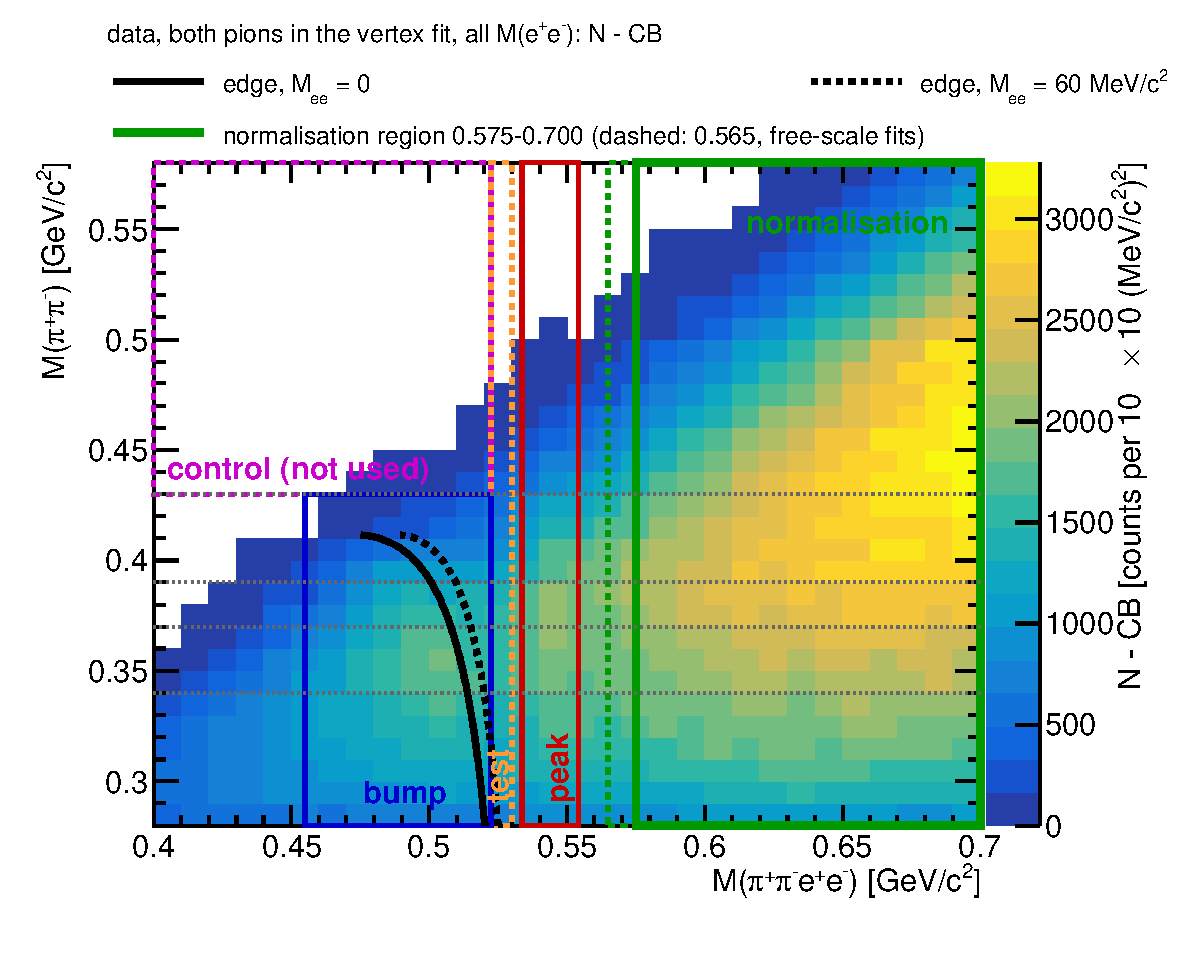
\includegraphics[width=0.46\textwidth]{figs_all/wp3_map_cnt_plain2.pdf}\\
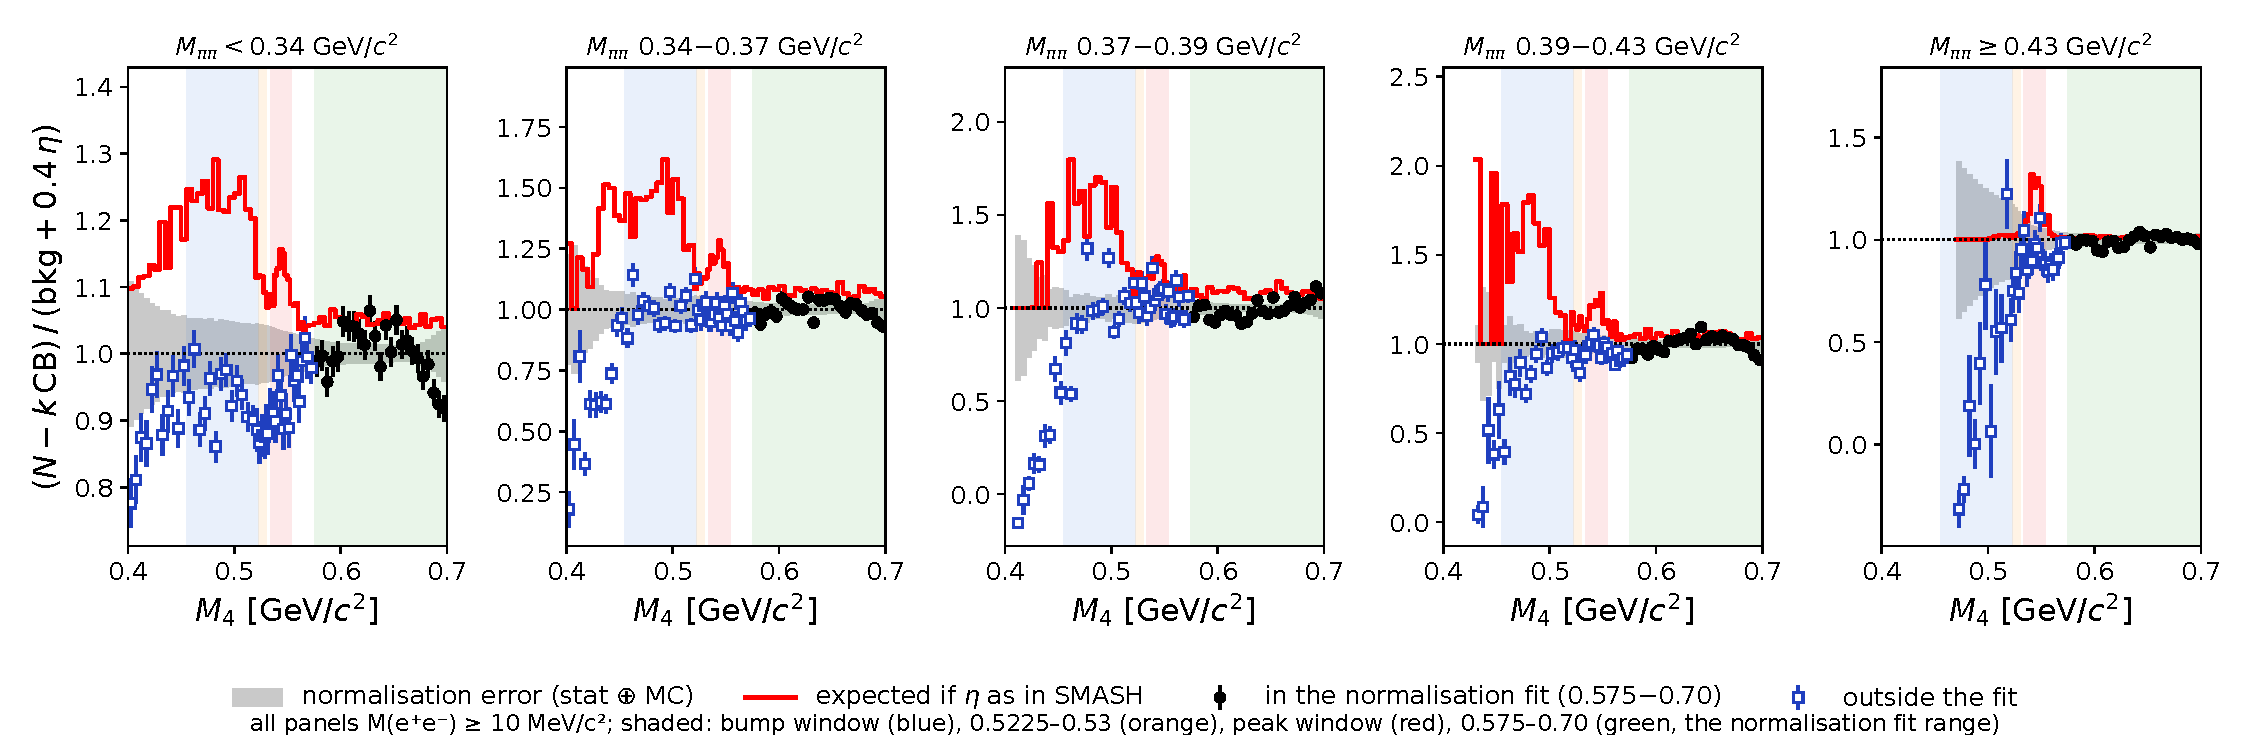
\includegraphics[width=\textwidth]{figs_all/fix_C2_plain2.pdf}
\caption{\textbf{What it shows: above the peak the normalised model matches the data in every \Mpipi slice; below the peak the carried-down
background is too high.} Top: data minus CB in \Mfour $\times$ \Mpipi, with the bump and peak windows, the normalisation region
0.575--0.70\,\GeVcc (green; dashed green line: 0.565\,\GeVcc, the lower edge used by the fits with a free scale per channel), the control
region \Mpipi$\ge0.43$\,\GeVcc, \Mfour 0.40--0.5225\,\GeVcc (not used: it failed its tests) and the test region 0.5225--0.5300\,\GeVcc;
lines: the bump edge for \Mee $=0$ and 60\,\MeVcc. Bottom: per \Mpipi slice, \Mee$\ge10$\,\MeVcc, data minus $0.954\times$CB over
(normalised background $+$ $0.4\times$ SMASH $\eta$); black full: bins of the normalisation fit, blue open squares: outside it; grey: error of the
normalisation (stat $\oplus$ MC); red: with the $\eta$ at SMASH instead of $\times0.4$; shaded: bump window (blue), test region (orange), peak
window (red), normalisation region (green). Raw counts on both sides.
\Sel data: \selnom; top all \Mee, bottom \Mee$\ge10$\,\MeVcc in \slicesfive; \cbspread. SMASH: \smashsel.
\figlabels{$k$: the CB factor (0.954); $M_4$: \Mfour.}}
\label{fig:normregion}
\end{figure}

%======================================================================
\section{How reliable the methods are: tests on simulated pseudo-data}
\label{sec:closure}
%======================================================================
\inshort{on simulated pseudo-data with a known truth only the peak side-band method recovers the truth within the allowed bias; the template fits
are biased by about $-10$\,\% and are cross-checks only.}
Pseudo-data with a known truth at the data luminosity (500 per scenario, with the realistic noise of the simulated templates) show that the
template fits are biased by about $-10$\,\% (noisy signal templates pull the fitted amplitude down) and limited by the simulation statistics:
they are cross-checks (Fig.~\ref{fig:templatefit}). The peak side bands pass (bias 0.5\,\%); the background-subtracted bump area fails
marginally ($-5.8$\,\% in one scenario against an allowed 5\,\%). With templates and pseudo-data taken from different halves of the simulation,
no method passes, the peak side bands included ($+14$\,\% in one scenario). On the data themselves, the side-band method applied at 13 windows
above the peak, where there is no $\eta$, gives pulls with an rms of $1.14^{+0.37}_{-0.59}$: a systematic term of 4.7\,\% of the peak yield
(Fig.~\ref{fig:displaced}).

\begin{figure}[!htbp]
\centering
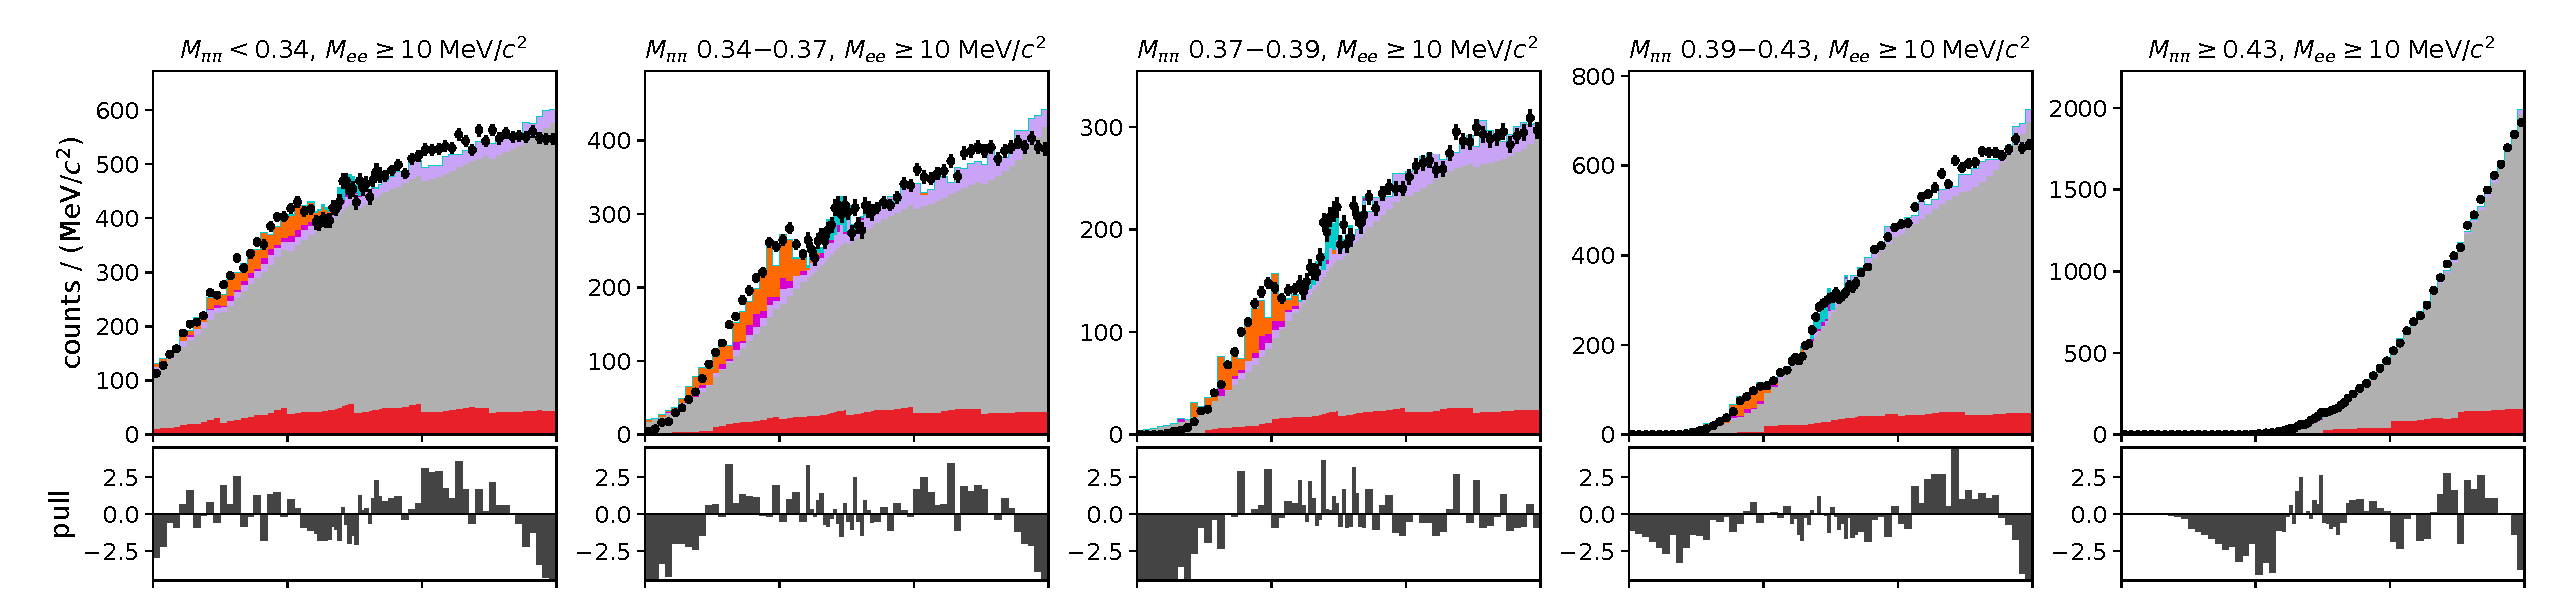
\includegraphics[width=\textwidth]{figs_all/fix_E1_cnt_plain2_crop.pdf}
\caption{\textbf{What it shows: the template fit (a cross-check) describes the shape of the data in every \Mpipi slice only roughly
($\chi^2$/ndf 2.59) and gives an $\eta$ scale of $0.382\pm0.017\pm0.040$, close to the main result.} The fitted class \Mee$\ge10$\,\MeVcc in the
five \Mpipi slices: data $N$ (black), CB (red), normalised non-$\eta$ background (grey), other $\eta$ decays (violet), converted photons of bump and
peak (magenta), \piz Dalitz bump (orange), direct decays (cyan) at the fitted amplitudes; pulls below.
\Sel data: \selnom; \Mee$\ge10$\,\MeVcc; \Mfour 0.40--0.70\,\GeVcc (5\,\MeVcc bins, 2.5\,\MeVcc in 0.520--0.570\,\GeVcc) in \slicesfive;
\cbspread, its factor constrained to $1\pm0.05$; $L=6079.2\,\nbinv$. SMASH: \smashsel; non-$\eta$ shapes smoothed (exponential of a cubic polynomial).}
\label{fig:templatefit}
\end{figure}

\begin{figure}[!t]
\centering
\begin{minipage}[c]{0.42\textwidth}
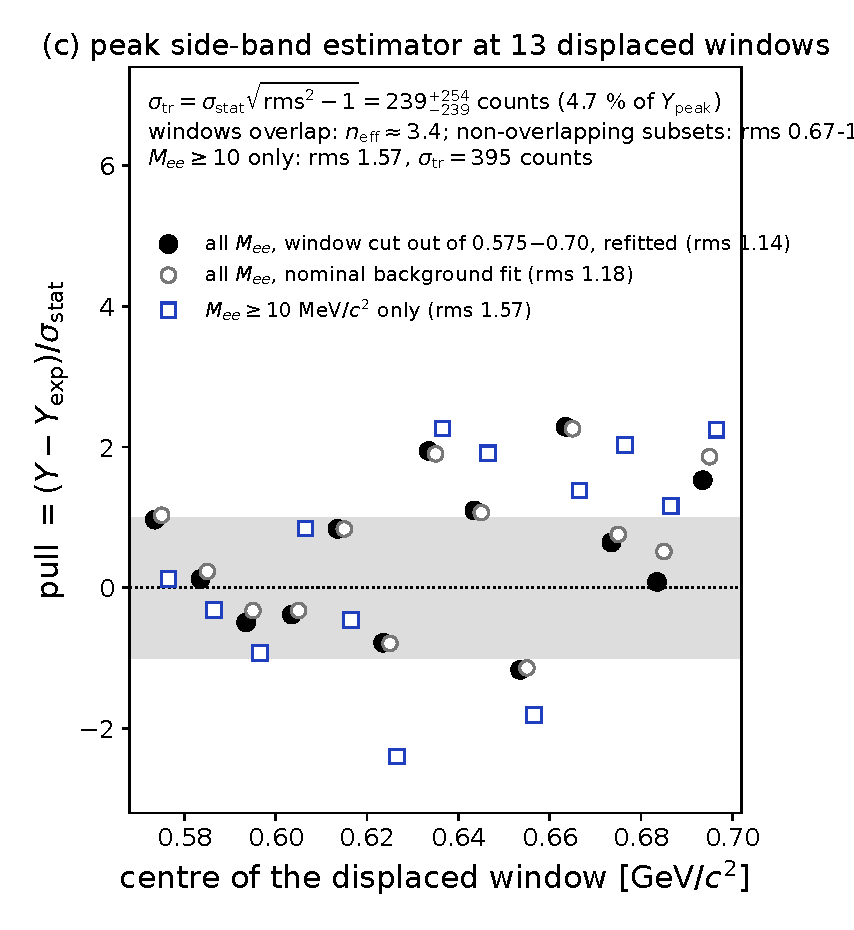
\includegraphics[width=\textwidth]{figs_all/fix_E4cd_cnt_plain_crop_cairo.pdf}
\end{minipage}\hfill
\begin{minipage}[c]{0.56\textwidth}
\caption{\textbf{What it shows: the side-band method applied where there is no $\eta$ finds none: the pulls scatter around zero with an rms close
to 1, and the extra spread is 239 counts (4.7\,\% of the peak yield), counted as a systematic error.} One panel, (c), of a larger figure. The
side-band estimator at 13 overlapping windows of the same width as the peak window, displaced to 0.58--0.70\,\GeVcc: pull $=$ (found $-$
expected)/stat error. Black: all \Mee, the displaced window cut out of the background normalisation region 0.575--0.70\,\GeVcc, which is
refitted (rms 1.14); open: all \Mee with the nominal normalisation (rms 1.18); blue squares: \Mee$\ge10$\,\MeVcc only (rms 1.57; 395 counts).
\Sel data: \selnom; \cbspread; windows of the same widths as for the peak (37.8\,\MeVcc in all) centred at 0.575, 0.585, \dots,
0.695\,\GeVcc; $L=6079.2\,\nbinv$.
\figlabels{$\sigma_{\mathrm{tr}}=\sigma_{\mathrm{stat}}\sqrt{\mathrm{rms}^2-1}$: the extra spread; $Y$, $Y_{\mathrm{exp}}$: found and
expected yield; $Y_{\mathrm{peak}}$: peak yield; $n_{\mathrm{eff}}\approx3.4$: effective number of independent windows; the line on
non-overlapping subsets of windows, cut at the right edge, reads rms 0.67--1.40.}}
\label{fig:displaced}
\end{minipage}
\end{figure}

%======================================================================
\section{Yields and systematic uncertainties}
\label{sec:yields}
%======================================================================
\inshort{the $\eta$ peak is measured with an 11.5\,\% systematic uncertainty (5088 counts); the bump is measured through its kinematic edge in $u$
(0.426 of SMASH with the \piz Dalitz angle corrected, 8.0\,\% systematic; per slice 0.423, 9.0\,\%, limited by the simulation statistics); only the
background-subtracted bump area is not determined (157\,\%).}
\begin{table}[!htbp]
\centering
\caption{Yields (raw counts $\times64/63$, not corrected for efficiency) and $\eta$ scales relative to SMASH (PDG 2020 branching ratios of the
simulation). stat includes the CB and the background normalisation; MC: simulation statistics; syst from Table~\ref{tab:syst} (for peak/SMASH the
\sigeta systematic without the make-up of the peak: 16.0\,\% $\oplus$ 8.8\,\% from the peak tail; 0.153 with it). ``Angle corrected'': the \piz
Dalitz decay angle corrected by a QED weight per count; every edge value includes the peak-tail term. Data: \selnom; \cbspread; \lumisel; windows:
bump 0.4550--0.5225, peak 0.53364--0.55416\,\GeVcc. SMASH: \smashsel.}
\label{tab:yields}
\small
\resizebox{\textwidth}{!}{%
\begin{tabular}{@{}l l r r r r@{}}
\toprule
quantity & method & value & stat & syst & MC \\
\midrule
$\eta$ peak yield, all \Mee & peak side bands (main result) & 5088 & 432 & 584 & 245 \\
$\eta$ peak / SMASH & peak side bands & 0.418 & 0.035 & 0.076 & 0.025 \\
\midrule
bump $\eta$ scale, edge in $u$ & as simulated & 0.390 & 0.018 & 0.029 & 0.027 \\
bump $\eta$ scale, edge in $u$ & angle corrected: the bump result & 0.426 & 0.020 & 0.034 & 0.030 \\
visible bump yield, bump window, all \Mee & edge in $u$ $\times$ SMASH bump & 21\,468 & 1003 & 1708 & 1347 \\
double ratio peak/bump & side bands / edge in $u$ (with the peak-composition term) & 0.97 & 0.09 & 0.35 & 0.09 \\
bump $\eta$ scale, edge per \Mpipi slice & as simulated & 0.392 & 0.021 & 0.035 & 0.042 \\
bump $\eta$ scale, edge per \Mpipi slice & angle corrected: cross-check & 0.423 & 0.023 & 0.038 & 0.048 \\
visible bump yield, bump window, all \Mee & edge per slice $\times$ SMASH bump & 21\,445 & 1152 & 1900 & 2223 \\
double ratio peak/bump & side bands / edge per slice (no peak-composition term) & 0.97 & 0.10 & 0.17 & 0.12 \\
\midrule
\multicolumn{6}{@{}l}{\emph{Not determined: the background-subtracted bump area (background extrapolated from above the peak)}} \\
bump area, \Mee$\ge10$\,\MeVcc & background subtracted & 7822 & 456 & 12\,870 & 1920 \\
bump area, all \Mee & extrapolated with the simulated share 0.477 & 16\,389 & 1129 & 25\,770 & 4110 \\
bump area / SMASH, \Mee$\ge10$\,\MeVcc / all \Mee & background subtracted & 0.312 / 0.299 & 0.018 / 0.021 & 0.52 / 0.47 & 0.076 / 0.075 \\
double ratio peak/bump area & side bands / bump area & 1.40 & 0.15 & 0.94 & 0.53 \\
\midrule
$\eta$ scale & template fit (cross-check) & 0.382 & 0.017 & 0.21 & 0.040 \\
\bottomrule
\end{tabular}}
\end{table}

\begin{table}[!htbp]
\centering
\caption{Systematic uncertainties in per cent. Each source counts its largest variation, after subtracting its statistical and template noise;
sources add in quadrature; MC and normalisation are separate. Columns: background-subtracted bump area (all \Mee, extrapolated; not determined),
peak yield, $\eta$ scale and BR$(\eta\to\ppee)$ of the template fits (cross-checks), double ratio peak/bump area (not determined), \sigeta. The
peak-tail term is counted for \sigeta and listed in parentheses for the peak yield; for \sigeta the efficiency term includes the make-up of the
peak. Data: \selnom; \lumisel.}
\label{tab:syst}
\small
\resizebox{\textwidth}{!}{%
\begin{tabular}{@{}l r r r r r r@{}}
\toprule
source & bump area & peak yield & $\eta$ scale, template fit & BR, template fit & double ratio & \sigeta \\
\midrule
normalisation region & 41.3 & 5.6 & 0 & 0 & 7.7 & 5.6 \\
background model & 138.5 & 5.7 & 37.4 & 18.3 & 46.2 & 5.7 \\
background shape from SMASH & 43.9 & 2.0 & 34.1 & 116.5 & 13.3 & 5.6 \\
fit range and binning & 19.6 & 0.4 & 12.0 & 24.3 & 22.7 & 0.4 \\
mass scale and resolution of the simulation & 6.6 & 5.7 & 4.3 & 7.0 & 4.3 & 9.0 \\
$\eta$-decay physics weights & 0.7 & 2.6 & 1.5 & 12.5 & 6.4 & 7.0 \\
scale of the other $\eta$ decays & 7.7 & 1.0 & 9.1 & 28.8 & 2.9 & 1.0 \\
pseudo-data closure & 37.6 & 4.7 & 10.1 & 14.8 & 37.9 & 4.7 \\
selection & -- & -- & 1.7 & 16.4 & 0 & 0 \\
efficiency model (+ make-up of the peak) & 3.4 & 0.1 & 12.2 & 8.6 & 10.2 & 31.8 \\
low-mass tail of the $\eta$ peak, $t=1\pm0.5$ & -- & (3.8) & -- & -- & -- & 8.8 \\
other (CB, simulated signal shapes) & 5.8 & 1.1 & 2.7 & 0 & 3.1 & 1.1 \\
\midrule
total systematic & 157.4 & \textbf{11.5} & 55.4 & 126.9 & 67.1 & \textbf{36.6} \\
stat / MC & 6.9 / 25.1 & 8.5 / 4.8 & 4.4 / 10.4 & 13.9 / 25.0 & 10.9 / 38.2 & 8.5 / 5.9 \\
\bottomrule
\end{tabular}}
\end{table}

The peak is measured (11.5\,\%); the background under the bump is not under control (a quadratic term or a different edge of the normalisation
region moves the bump area by 40--150\,\%), so the bump area and its double ratio are not determined. \sigeta carries the make-up of the peak
(32\,\%). Between the four beam periods the peak, the template-fit scale and the bump area pass the stability test ($p=0.04$--0.99); the
bump edges are marginal but pass ($p>0.01$): in $u$ $p=0.024$ between the periods and $z=-2.1$ between the two halves of the data, per slice
$p=0.07$ and 0.05.

\textbf{The bump in $u$.} Fit range $-45\le u<45$\,\MeVcc (36 bins of 2.5\,\MeVcc, \Mpipi 0.30--0.40\,\GeVcc), the step smeared by the simulated
resolution (6.7\,\MeVcc), the $\eta$ peak fixed at 0.418 $\times$ its SMASH shape ($\pm0.08$ on it moves the result by 0.02\,\%); the bump scale is the
ratio of the data step to the step of the same fit on the SMASH bump channels. Systematic terms in per cent of the result: data/SMASH resolution
ratio 4.5; step that a smooth background projects onto the edge 4.0; the peak term with its low-mass tail 3.4; CB 2.6 (it covers the like-sign
step); fit model 1.9; physics weights 1.5; the rest 1.0 or less (among them the \piz Dalitz angle correction, 0.3); total \textbf{8.0}, against
stat 4.8 and MC 7.0 (total 11.6\,\%). Not counted: Dalitz plots of $\eta\to\pipi\piz$ with phase space only ($+6$ to $+8$\,\%; excluded by KLOE-2
and by the data) and an edge without the \Mee term ($+5.9$\,\%; kinematically wrong for Dalitz pairs). Pseudo-data (21 truths $\times$ 1000):
closure within $\pm2$\,\% for smooth backgrounds, pull widths 0.95--1.07. Checks: the four \Mpipi slices agree ($\chi^2$ 1.0/3; four separate fits
give $0.429\pm0.020\pm0.032$), \Mee below / above 10\,\MeVcc 0.411 / 0.444; no step in the simulated non-$\eta$ backgrounds nor in a data region
without bump (\Mpipi 0.42--0.46\,\GeVcc, $3\pm17$ counts); beam periods $p=0.024$, two halves of the data $z=-2.1$ (marginal).

\textbf{The bump edge per \Mpipi slice} (cross-check). Statistical error 0.021, MC error 0.042. Systematic terms in per cent (as simulated / angle
corrected / conversions $\times0.48$): edge model 1.1 / 1.4 / 0; \Mpipi slices 2.9 / 2.9 / 3.8; mass transfer and resolution 4.3 / 4.3 / 4.4;
CB 1.3; physics weights 1.2 / 1.2 / 1.1; selection 0 / 0 / 2.1; step of a smooth background 6.0 (of unknown sign); \piz Dalitz angle correction
-- / 0.2 / 0.3; share of converted photons from the peak -- / -- / 7.2; peak tail 3.4 / 3.7 / 4.9; total \textbf{8.9 / 9.0 / 12.4}, against
stat 5.4 and MC 10.9--14.7 (angle corrected: total 15.4\,\%). Pseudo-data: bias at most 1.6\,\% with the true templates, $+2$ to $+6$\,\% with
noisy templates; only a background structure as narrow as the edge (a 10\,\% bump of 15\,\MeVcc: $+21$\,\%) would bias it, and none is seen
(data slice without a bump: $15\pm15$ counts). Beam periods $p=0.07$, halves $p=0.05$ (marginal). The angle correction raises the scale by
8.1\,\% (0.392 $\to$ 0.423); with the conversions $\times0.48$ (from the peak) it is 0.569. The like-sign counts show no step in \Mfour per slice
($0.5\pm25.6$, base selection), unlike the $e^-e^-$ counts in $u$: there the edge has its \Mee term, which a slice in \Mfour smears out.

%======================================================================
\section{SMASH with a free scale per channel}
\label{sec:freescale}
%======================================================================
\inshort{every SMASH component gets its own free scale; the $\eta$ signal channels share one scale ($0.46\pm0.06$), the non-$\eta$ background
above the peak is 10--30\,\% above SMASH with an undetermined split, and the model is incomplete ($p<0.001$). A description, not measurements.}
Data $=$ CB $\times$ a factor ($1\pm0.05$) $+$ the sum of the SMASH components, each with its own free scale, in 350 bins (\slicesfive,
\Mee$\ge10$\,\MeVcc, \Mfour 0.40--0.70\,\GeVcc): the \piz Dalitz bump, the converted-photon bump, the converted photons of the peak, the direct
decays, the other $\eta$ decays, the background without a conversion pair split into pions from $\omega/\rho^0$ and the rest, and the background
with a conversion pair. The template noise of the simulation enters the fit weights. SMASH as it is gives $\chi^2$ 1789 (full covariance) for 350 bins.

\begin{table}[!htbp]
\centering
\caption{\textbf{What it shows: every scale of the fit with a free scale per channel, what fixes it and how far it can be trusted.} Scales relative
to SMASH as it is (value $\pm$ stat $\pm$ MC); what fixes them (share of the Fisher information from the bump window 0.4550--0.5225, the peak window
0.53364--0.55416 or the region 0.565--0.70\,\GeVcc above the peak); the bias test on pseudo-data with the real template noise; the range when the
weight of the template noise in the fit runs from 0.5 to 1.5; the reading. Data: \selnom; \Mee$\ge10$\,\MeVcc; \Mfour 0.40--0.70\,\GeVcc in
\slicesfive; \cbspread; \lumisel. SMASH: \smashsel.}
\label{tab:freescale}
\footnotesize
\setlength{\tabcolsep}{2.5pt}
\begin{tabularx}{\textwidth}{@{}>{\raggedright\arraybackslash}p{3.6cm} l l l l L@{}}
\toprule
SMASH component & value $\pm$ stat $\pm$ MC & fixed by & bias test & weight 0.5--1.5 & reading \\
\midrule
bump, \piz Dalitz decay & $0.412\pm0.021\pm0.065$ & bump 82\,\% & $-20$\,\%, fail & 0.37--0.41 & one $\eta$ scale with the two peak channels \\
bump, converted photon & $-0.087\pm0.067\pm0.228$ & bump 74\,\% & fail & 0.14 to $-0.13$ & not determined \\
peak, $\eta\to\pipi\gamma$ converted & $0.335\pm0.158\pm0.155$ & peak 75\,\% & $-58$\,\%, fail & 0.35 & weak; one $\eta$ scale \\
peak, direct decays & $0.626\pm0.064\pm0.099$ & peak 96\,\% & $+1$\,\%, pass & 0.57--0.67 & determined, $\pm{\approx}0.1$ model/method \\
other $\eta$ decays & $2.102\pm0.072\pm0.584$ & above 76\,\% & $-15$\,\%, fail & 1.52--2.96 & not determined \\
no conversion pair, $\omega/\rho^0$ pions & $0.788\pm0.050\pm0.275$ & above 98.5\,\% & $-15$\,\%, fail & 0.58--1.10 & not determined \\
no conversion pair, other pions & $1.109\pm0.030\pm0.107$ & above 77\,\% & $+4$\,\%, marginal & 1.06--1.18 & close to SMASH \\
with a conversion pair & $1.596\pm0.122\pm0.674$ & above 85\,\% & $+5$\,\%, pass & 2.11--0.83 & not determined \\
CB factor & $0.907\pm0.045\pm0.043$ & constraint & $-1$\,\%, pass & 0.90--0.92 & nuisance \\
\bottomrule
\end{tabularx}
\end{table}

\textbf{Plain conclusions.} (1) The \piz Dalitz bump, the converted photons of the peak and the direct decays share one $\eta$ scale,
$0.456\pm0.058$ ($p=0.21$), $0.571\pm0.071$ after the template-noise correction ($p=0.51$). (2) The direct decays give $0.63\pm0.12\pm{\approx}0.1$
(0.44--0.94 over the variants); their ratio to the \piz Dalitz bump is within 1--2$\sigma$ of the PDG ratio (1.52 here, 1.98 with \Mee$<10$\,\MeVcc).
(3) The non-$\eta$ background in 0.565--0.70\,\GeVcc is 10--30\,\% above SMASH (1.15 for the whole non-$\eta$ background here, 1.11--1.28 over tied
fits); its split is not determined (the conversion-pair scale is anti-correlated with the others at $-0.82$ to $-0.88$). (4) The converted photons
need \Mee$<10$\,\MeVcc (0.32--0.34 there), provided a CB-like term is added for that class (its factor in this fit $4.4\pm1.6$). (5) The template noise dominates (MC
1--8 $\times$ stat). (6) Above \Mfour$=0.70$\,\GeVcc the scaled components fail (CB factor 1.38--1.42, conversion-pair scale $-2.3$ or 0): the scales
must not be carried there. (7) The model is incomplete: $\chi^2$ 603.6/342 against $356\pm33$ for a perfect model (largest of 2000 pseudo-experiments: 461),
$p<0.001$; the fitted model is $+2.0$\,\% above the data ($+5.8$\,\% in the peak window), and the scales move with the fit weights far beyond their
errors (other $\eta$ decays 1.1--3.9, conversion pairs 2.4--0; \piz Dalitz bump 0.31--0.41, direct decays 0.48--0.69).

%======================================================================
\section{Physics quantities}
\label{sec:phys}
%======================================================================
\inshort{$\sigeta=0.43\pm0.17\,(\mathrm{measurement})\,^{+0.08}_{-0.03}\,(\mathrm{production~model})$\,mb, 0.40 of SMASH (preliminary); the
requirement of an event vertex keeps the $\eta$ (0.994); HGeant's isotropic decay angle makes the simulated bump efficiency about 16\,\% too high.}

\subsection*{\texorpdfstring{$\eta$}{Eta} efficiency of the event-vertex requirement}
Every count must have a reconstructed event vertex ($\vz>-500$\,mm); the target-region cut $\vz>-160$\,mm comes on top of it and acts alike in
data and simulation (Conventions). The vertex finder, the same in data and simulation, makes a vertex only if
at least two tracks point into $-170<z<-30$\,mm, $r<20$\,mm. The vertex requirement removes 32\,\% of the \ee counts of the data (0.565 survive in the peak window)
but 0.03\,\% of the simulated $\eta$ entries. The counts were read from the 29 daily data files without any vertex requirement and split into events
with and without a vertex, each class with its own like-sign CB; the $\eta$ content of each class was measured in three ways (the peak content, the
ECAL-tagged $\eta$ and the bump edge step), and the efficiency is with/(with $+$ without), combined with inverse-variance weights (the ECAL tag
carries 81\,\% of the weight).

\begin{minipage}[t]{0.52\textwidth}\vspace{0pt}
\captionof{table}{$\eta$ efficiency of the requirement of a reconstructed event vertex, $\vz>-500$\,mm (data counts, not normalised; simulation unweighted). The peak content
with the standard CB is a CB fluctuation ($e^+e^+$ counts without vertex 2.4$\sigma$ low), shown but not used; the smooth CB is a polynomial fit of
the like-sign counts. Data: \selnovtx; no target-region cut and no pion-vertex condition.}
\label{tab:vtx}
\footnotesize
\setlength{\tabcolsep}{2pt}
\begin{tabular}{@{}l r r l@{}}
\toprule
measure & with & without & efficiency \\
\midrule
peak, standard CB & 4657 & 902 & $0.838\pm0.063$ \\
peak, no CB & 4646 & 165 & $0.966\pm0.065$ \\
peak, smooth CB & 4670 & 263 & $0.947\pm0.063$ \\
ECAL tag & 3297 & $-4\pm77$ & $1.001\pm0.023$ \\
edge step & 1241 & $21\pm96$ & $0.983\pm0.075\pm0.028$ \\
\textbf{combined} (smooth CB) & & & $\mathbf{0.994\pm0.021}$ \\
combined, standard CB & & & $0.990\pm0.022$ \\
\midrule
SMASH, peak & & & 0.9997 \\
SMASH, bump & & & 0.9986 \\
counts kept, peak / all & & & \multicolumn{1}{@{}l@{}}{0.565 / 0.677} \\
\bottomrule
\end{tabular}
\end{minipage}\hfill
\begin{minipage}[t]{0.45\textwidth}\vspace{0pt}
\small\raggedright
\textbf{Origin of the counts without a vertex.} 87\,\% of their pion pairs cross 8\,mm or more from the beam axis (35\,\% with a vertex);
their pp-elastic content is $0.028\pm0.003$ of the cell's; CB$/N$ is 0.58 (0.13 with a vertex). So they are mostly non-target events. Their
pions cross near $z\approx-200$\,mm, 5--6\,cm in front of the hydrogen cell, where the simulated geometry has the steel holder, beam tube and
flanges; beam halo on this material is a hypothesis. The simulation has no such events.\\[0.3em]
\textbf{Conclusion.} The correction simulation/data is $0.9997/0.994=1.006\pm0.021$ for \sigeta (bump $1.00\pm0.02$; ratios free of it): not applied,
one-sided $+2$\,\% ($+4$\,\% at 95\,\% CL). The cut is validated. It is \emph{not} the cause of the low \sigeta: 0.93\,mb would need an efficiency of
0.46, excluded by the ECAL tag at 23$\sigma$ and by the edge step at 6.6$\sigma$. K$^0_S$: 0.72--0.85 (displaced pions).
\end{minipage}

\begin{figure}[!htbp]
\centering
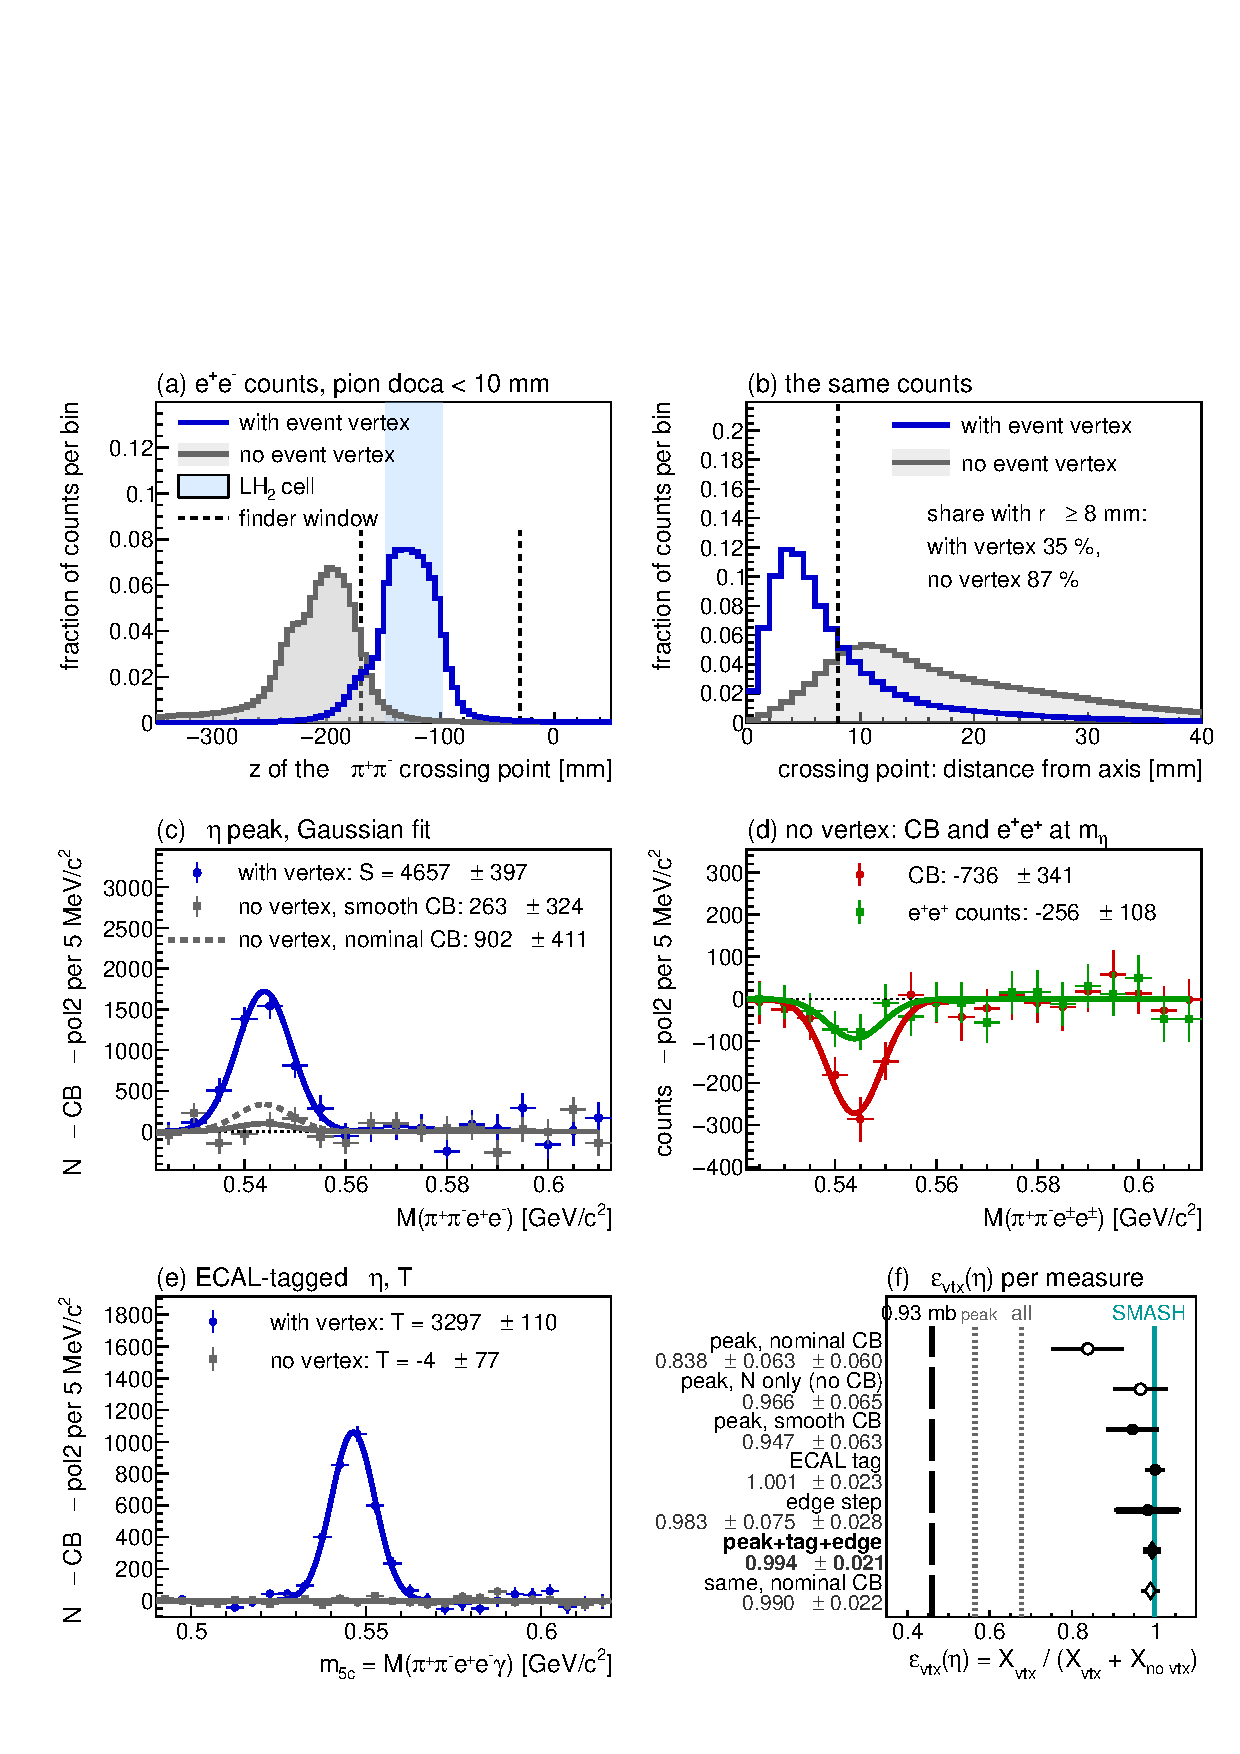
\includegraphics[width=0.72\textwidth]{figs_all/fix2_vtx_fig_cnt_plain.pdf}
\caption{\textbf{What it shows: counts without an event vertex hold no tagged $\eta$, so the vertex requirement keeps practically all the $\eta$, far
from the 0.46 that \sigeta $=0.93$\,mb would need.} Counts with an event vertex blue, without grey. (a, b) $z$ and distance from the beam axis of
the crossing point of the two pions (dashed: the $z$ window of the vertex finder, and 8\,mm; the $z$ of the counts without a vertex is partly
shaped by the selection; shaded: the liquid-hydrogen cell). (c) $\eta$ peak, data minus CB minus the second-order polynomial of a Gaussian fit:
with a vertex; without a vertex with a smooth like-sign CB (squares: one variant; legend: mean of the 12) and with the standard CB (dashed).
(d) Without a vertex: the CB and the $e^+e^+$ counts dip at $m_\eta$. (e) ECAL-tagged $\eta$: 3297 with and $-4\pm77$ without a vertex. (f)
Efficiency per measure as in Table~\ref{tab:vtx} (edge step: thick bar stat $\times1.2$, thin bar with the model rms) and combined,
$0.994\pm0.021$; lines: simulation 0.9997, survival of the counts in the peak window and in all \Mfour (0.565 / 0.677), and 0.46, the value that
\sigeta $=0.93$\,mb would need.
\Sel data read from the 29 daily data files without any vertex requirement: \selnovtx; no target-region cut and no pion-vertex condition;
with a vertex: $\vz>-500$\,mm, without: $\vz=-1000$\,mm (whole events split); each class with its own CB $=2\sqrt{N_{++}N_{--}}$ from its own
like-sign counts; (a, b) pion pairs with a distance of closest approach below 10\,mm; (c) fixed Gaussian (0.5439\,\GeVcc, 5.4\,\MeVcc) plus a
second-order polynomial in \Mfour 0.5225--0.61\,\GeVcc; (e) the ECAL photon cuts of Fig.~\ref{fig:res-ecals}; (f) edge step in the four \Mpipi
slices 0.30--0.34, 0.34--0.37, 0.37--0.39 and 0.39--0.40\,\GeVcc. Simulation: \smashsel.
\figlabels{$S$, $T$: peak content and number of tagged $\eta$; $\varepsilon_{\mathrm{vtx}}(\eta)=X_{\mathrm{vtx}}/(X_{\mathrm{vtx}}+X_{\mathrm{no\,vtx}})$:
the efficiency for a measure $X$; $m_{5c}$: $M(\ppee\gamma)$ with the photon rescaled; pion doca: distance of closest approach of the two pions.}}
\label{fig:vtx}
\end{figure}

\subsection*{Normalisation and corrections not applied}
The $\eta$ yields carry the correction for a trigger loss in one sector on the first beam days, 1.012, times one minus the target-wall share of the
$\eta$ signal, 0.97: $0.98^{+0.03}_{-0.04}$. The wall share of all counts (13--15\,\% of the data minus CB in 0.40--0.70\,\GeVcc) describes the
non-$\eta$ background and is \emph{not} applied to $\eta$ yields. On day 045 the elastic events show no deficit in that sector (share
$1.074\pm0.009$ relative to the clean days), so $L=6079.2\,\nbinv$ is unchanged; the deficit of the \ppee counts on that day ($0.903\pm0.007$) is
specific to the lepton channel (cause not studied). \emph{Known sign, not applied}: higher: trigger live time $+7.1$--7.3\,\%, event loss of the
START-based track sorter $+1.3$--2.8\,\%, counts whose momenta could not be corrected $+2.2$\,\% (together $\times1.109$--1.127: 0.48\,mb;
direct-decay value 0.58--0.59\,mb, 0.70\,mb with its side-band value per \Mee class), the measured vertex correction $1.006\pm0.021$ ($+2$\,\%,
$+4$\,\% at 95\,\% CL), $p_T$ reweighting $+21$\,\% (production model, kept apart: $^{+0.08}_{-0.03}$\,mb); lower: the data peak width (simulated
resolution $\times0.89$, $-10.8$\,\%), a target-wall share of the $\eta$ signal of 12\,\% ($-9$\,\%), $y$-only reweighting ($-8$\,\%).

\textbf{Make-up of the peak.} The data peak is richer in large-\Mee pairs than SMASH ($0.546\pm0.053$ of it at \Mee$\ge10$\,\MeVcc against 0.425): the
side bands per \Mee class and the X17 fit give an $\eta$ scale of 0.50 from the direct decays ($0.497\pm0.059$, stat) and 0.24 from the converted
photons ($0.237\pm0.049$), both with the PDG 2026 branching ratios; the peak value (0.409 with the same branching ratios, 0.418 with those of
the simulation) mixes both. Half their difference ($\pm32$\,\%) is the composition systematic of \sigeta; which SMASH
component is wrong is open. The bump does not decide: the edge gives 0.426 in $u$ (0.423 per slice) with the simulated conversion rate and 0.549
(0.569) with the conversions $\times0.48$, and its own \Mee split cannot fix the converted-photon share; the ECAL tag (0.454 $\pm$ 0.043), from close
\piz Dalitz pairs of the same decay, lies near the direct-decay value, but its prediction moves by a factor 1.46 with the photon energy scale, so today
it favours neither. If the data lose close pairs more than the simulation (\S\ref{sec:notdet}), the direct decays at larger \Mee would be the most
reliable $\eta$ scale, \sigeta $\approx0.52\pm0.06\,(\mathrm{stat})$\,mb; until then 0.43\,mb with its $\pm32$\,\% stands.

\textbf{Literature.} No published inclusive \sigeta exists at this energy. HADES at 3.5\,GeV published $1.14\pm0.20$\,mb (PYTHIA) and $0.93\pm0.14$\,mb
(UrQMD) (Eur.\ Phys.\ J.\ A 48 (2012) 64); the value here is 0.38--0.46 of those, although the cross section should rise with energy, and a
preliminary ECAL analysis of the same beam time showed 1.15--1.72\,mb (no errors). The efficiency of the event-vertex requirement is measured and excluded as the cause. The
one-sided items alone raise the value only to 0.48\,mb (0.50\,mb with the vertex correction at its 95\,\% bound); with the direct-decay value they
give 0.58--0.59\,mb (0.70\,mb with its side-band value per \Mee class), and with that value and the $p_T$ item in addition 0.85\,mb, compatible
with $0.93\pm0.14$\,mb. No significance is quoted, because the make-up of the peak ($\pm32$\,\%) is not resolved.

\textbf{Simulation finding.} HGeant decays the virtual photon of the \piz Dalitz decays of the bump isotropically instead of $1+\cos^2\theta^*$
(Fig.~\ref{fig:res-qed}). It is not corrected in the template fits and the bump area (known-sign systematic: template-fit $\eta$ scale
$+9$/$+12$\,\%, its BR $-7$/$-9$\,\%, double ratio $-8$/$-10$\,\%; \sigeta from the peak unchanged). In the bump-edge values every simulated \piz
Dalitz entry carries its own QED weight, averaged over the circle on which its lost photon must lie; the effective factors are
$0.861\pm0.007\,(\mathrm{sim.\ stat.})\pm0.004\,(\mathrm{model})$ ($u$) and $0.860\pm0.010\pm0.004$ (per slice), depending on the softer lepton
(0.91 at 60--100\,MeV/$c$, 0.80--0.82 above 200\,MeV/$c$). Result: $+9.2$\,\% in $u$ (0.390 $\to$ 0.426) and $+8.1$\,\% per slice
(0.392 $\to$ 0.423); the bump \sigeta is 0.444 / 0.442\,mb.

%======================================================================
\section{X17}
\label{sec:x17}
%======================================================================
\inshort{no X17 signal: $r<0.114$, i.e.\ $\BRX<3.16\times10^{-5}$ at 17\,\MeVcc (90\,\% CL$_s$, PDG 2026); about two times weaker than BESIII near
17\,\MeVcc and numerically similar to the HADES preliminary value, which is built differently and is not a cross-check.}
\begin{table}[!htbp]
\centering
\caption{\textbf{What it shows: the limit at 17\,\MeVcc for each way of tying the X17 yield and each variant.} 90\,\% CL$_s$ upper limits
[$10^{-5}$] at 17.0\,\MeVcc (16.7 and 16.85 within 0.02), PDG 2026. Expected: pseudo-experiments fixed before the opening, median [68\,\%].
Data: \selnom; fit in \Mfour 0.5225--0.6100\,\GeVcc $\times$ \Mee 2--62\,\MeVcc; CB from the like-sign data; $L=6079.2\,\nbinv$;
SMASH shapes of the $\eta$ channels.}
\label{tab:x17limits}
\small
\begin{tabular}{@{}l r l@{}}
\toprule
X17 yield tied to & observed & expected \\
\midrule
fitted direct-decay yield (nominal) & \textbf{3.16} & 2.68 [1.54, 4.92] \\
fixed $\eta$ scale 0.38 & 3.29 & 2.60 [1.55, 4.47] \\
$\eta$ scale of the peak & 2.81 & 2.25 [1.42, 3.56] \\
\midrule
nominal, PDG 2020 & 3.06 & 2.60 [1.50, 4.77] \\
nominal, vector-like ($1+\cos^2\theta$) & 3.79 & \\
nominal, template-noise offset & 3.35 & \\
Feldman--Cousins interval & [0, 3.55] & \\
Bayesian, flat prior & 4.10 & \\
\bottomrule
\end{tabular}
\end{table}

\textbf{Method.} A two-dimensional Poisson likelihood of \Mfour (0.5225--0.610\,\GeVcc) $\times$ \Mee (2--62\,\MeVcc): a free background in every
\Mee bin, the CB from the like-sign data, the $\eta$ channels with their SMASH shapes, and the X17 yield tied to the fitted direct-decay yield. The
procedure and the expected limit were fixed on the \Mee side bands before the region 12--28\,\MeVcc was opened, with BR$(\eta\to\ppee)=2.68\times10^{-4}$
(PDG 2020); the limits are quoted with $2.76\times10^{-4}$ (PDG 2026), which moves $r$ at the limit by $+0.13$\,\%. Fit of all 1050 cells:
$\chi^2$/ndf 0.993; fitted direct-decay yield $3659\pm503$ counts.

\textbf{Why not a simple count?} The Rolke method (W.~Rolke, A.~L\'opez, J.~Conrad, NIM A 551 (2005) 493, as in ROOT) gives a profile-likelihood
interval for one counting window. In the X17 window (\Mfour 0.5312--0.5566\,\GeVcc, \Mee 15.5--24.5\,\MeVcc) it sees $N=6424$ counts against a
predicted background of $6312\pm1196$ and gives fewer than 2083 X17 counts, i.e.\ $\BRX<2.6\times10^{-4}$: \textbf{about 8 times weaker} (8.3). Both are
frequentist methods with the systematic uncertainties as nuisance parameters (on our full likelihood the Feldman--Cousins interval is
$[0,\,3.55\times10^{-5}]$, close to the CL$_s$ limit), but the count must \emph{predict} the background in the window, with 19\,\% uncertainty (15
times the statistical error $\sqrt N\approx80$), while the two-dimensional fit \emph{measures} it in every \Mee bin from the \Mfour side bands and
separates the narrow X17 line from the smooth spectrum of the direct decays. The gain comes from the information used (the shape), not from the
statistical method.

\textbf{Variants} (Table~\ref{tab:x17limits}). The nominal way of tying the yield failed one of its tests on pseudo-experiments (a slope
test); tying it to the fixed $\eta$ scale gives 3.29 and is quoted next to it. Local significance at most $0.98\sigma$ (22\,\MeVcc),
0.49$\sigma$ at 17\,\MeVcc. At most 392 X17 counts. The simulation statistics add 11\,\%; the simulation replicas suggest the nominal is about
6\,\% optimistic (3.35). With \sigeta and its 39.2\,\% folded in, $\sigma\times\mathrm{BR}_X\mathrm{BR}_{ee}<15.6$\,nb (13.5\,nb plain product);
15.7\,nb with the measured vertex correction applied, 16.3\,nb at its 95\,\% bound (PDG 2026).





\floatbarrier
%======================================================================
\section{Open points, corrections and notation}
\label{sec:open}
%======================================================================
\textbf{Open points}: (1) the separate analysis of close \ee pairs: their efficiency at an opening angle of 0--6$^\circ$ in data and simulation,
from \piz, $\eta$ and $\omega$ Dalitz decays with the ECAL photon; (2) the make-up of the peak (which SMASH component is wrong; \sigeta 0.25 or
0.52\,mb); (3) a larger standard simulation and smoother signal templates (several results are limited by the simulation statistics), and at least
10 times more simulated $\eta\to\pipi\piz$ with the full ECAL simulation; (4) a bump-free control region below the peak, for the
background-subtracted bump area; (5) the QED decay angle of the \piz Dalitz decays in HGeant; (6) why the scaled SMASH components fail ($p<0.001$;
nothing above 0.70\,\GeVcc); (7) the class \Mee$<10$\,\MeVcc (its CB factor came out at 7.6--13.2 in the background normalisation fits; there SMASH with the measured scales is 1/0.65 too high,
Fig.~\ref{fig:res-ucompare}); (8) the scale of the other $\eta$ decays (0.47--2.6); (9) how true pairs with a ghost track should be counted
(8.5--14.5\,\% on the ratios before normalisation); (10) the production-model item of \sigeta, quoted apart ($^{+0.08}_{-0.03}$\,mb); (11) the
\Mee scale and resolution of the X17 line, unchecked on data; (12) which vertex condition the elastic luminosity used (about 1\,\% if it used
none); (13) the ECAL full reconstruction (photon energy scale, module efficiency, a photon cut free of START); (14) the size of the low-mass tail of the $\eta$ peak (the data allow $0.3\pm1.0$ of the simulated tail; until then
$t=1\pm0.5$).

{\footnotesize
\setlength{\tabcolsep}{4pt}
\renewcommand{\arraystretch}{1.0}
\begin{longtable}{@{}>{\raggedright\arraybackslash}p{3.6cm} >{\raggedright\arraybackslash}p{\dimexpr\textwidth-3.6cm-2\tabcolsep\relax}@{}}
\caption{\textbf{Corrections used} (what, how, size).}\label{tab:corr}\\
\toprule
correction & how / size \\
\midrule
\endfirsthead
\toprule
correction & how / size \\
\midrule
\endhead
\bottomrule
\endfoot
combinatorial background & like-sign data $2\sqrt{N_{++}N_{--}}$ in 10\,\MeVcc cells of \Mfour, shared out over \Mpipi slices and \Mee classes by the like-sign share / CB$/N$ 0.06 in the peak window \\
mass scale of the simulation & simulated \Mfour moved to $0.99615\,[m^{\mathrm{true}}+1.0\,(m-m^{\mathrm{true}})]$ ($m$: reconstructed, $m^{\mathrm{true}}$: true mass), \Mpipi$\times0.9952$ / ratios of the base selection $-1$ to $-2.5$\,\% \\
$\eta$-decay physics weights & measured $\eta$ decay matrix elements per simulated entry / direct decays in the peak window $\times1.04$ \\
leakage of the peak & the peak leaks into its side bands; corrected with the simulated leakage (0.154) and the background ratio window/side bands (1.186) / peak yield $+22$\,\% \\
bump area at all \Mee & measured at \Mee$\ge10$\,\MeVcc only; divided by the simulated share 0.477 (the area is not determined) \\
trigger loss in one sector & double ratio of counts with/without a track in sector 2, deficit days/clean days, days 034--045 / 1.012 (peak) \\
target-wall share of the $\eta$ & from the $\eta$ per count in the vertex slices (never the wall share of all counts) / $\times0.97$ \\
PDG 2026 & simulated channels rescaled (direct decays $\times1.030$) / \sigeta $-2.2$\,\%; X17 limit $\times1.031$ \\
make-up of the peak & half the difference of the direct-decay and converted-photon values in the data / \sigeta $\pm32$\,\% (systematic only, until the close-pair efficiency is measured) \\
\piz Dalitz decay angle (bump edges only) & every simulated \piz Dalitz bump entry weighted by its QED/isotropic ratio, averaged over the circle of its lost photon (effective 0.861 in $u$, 0.860 per slice, allowance $\pm0.004$) / bump scale $+9.2$\,\% ($u$), $+8.1$\,\% (per slice) \\
peak tail & the simulated low-mass tail of the $\eta$ peak kept, $t=1\pm0.5$ / systematic $\pm3.4$\,\% on the bump scale in $u$, $\pm3.7$\,\% per slice, $\pm8.8$\,\% on the peak scale and \sigeta \\
\end{longtable}
}

{\footnotesize
\setlength{\tabcolsep}{4pt}
\renewcommand{\arraystretch}{1.0}
\begin{longtable}{@{}>{\raggedright\arraybackslash}p{3.6cm} >{\raggedright\arraybackslash}p{\dimexpr\textwidth-3.6cm-2\tabcolsep\relax}@{}}
\caption{\textbf{Notation} used in this summary. The full report defines every item in detail.}\label{tab:nota}\\
\toprule
\endfirsthead
\toprule
\endhead
\bottomrule
\endfoot
count, event group & a count is one stored \ppee combination (one entry): every combination of tracks with the right charges whose four tracks pass the identification; an event can give more than one count. Event group: all counts of one event (the unit of all statistical errors) \\
base / nominal selection & PT3 trigger, a reconstructed event vertex in the target region, START-free particle identification, corrected momenta, all combinations that pass the identification / the same plus both pions used in the event-vertex fit (values in Section~\ref{sec:res}) \\
event vertex & reconstructed by the vertex finder from at least two tracks ($\vz>-500$\,mm; $\vz=-1000$\,mm if none); target region $\vz>-160$\,mm \\
$N$, $N_{++}$, $N_{--}$, CB & unlike-sign and like-sign counts; combinatorial background $2\sqrt{N_{++}N_{--}}$ from the like-sign data (sometimes with a fitted factor) \\
$L$, 64/63 & START-free luminosity of the analysed runs (6079.2\,\nbinv, $\pm6.9$\,\%); PT3 trigger-bit factor (63/64 of the PT3 events carry bit 8192) \\
stat, syst, MC, norm. & statistical (whole events, CB replicas), systematic, simulation statistics (100 bootstrap replicas of the simulation), normalisation \\
SMASH channels & bump: $\eta\to\pipi\piz$ with the \piz Dalitz decay or a converted photon, the other photon lost; peak: direct $\eta\to\ppee$ and $\eta\to\pipi\gamma$ with a converted photon; other $\eta$ decays; non-$\eta$ background without / with a conversion pair \\
windows (\Mfour, \GeVcc) & bump window 0.4550--0.5225; peak window 0.53364--0.55416; peak side bands 0.5250--0.5336 and 0.5542--0.5628; normalisation region of the background 0.575--0.70 (at \Mee$\ge10$\,\MeVcc); the region above the peak of the data/SMASH ratios and of the fits with a free scale per channel 0.565--0.70; test region 0.5225--0.5300; $\eta$ peak band 0.5325--0.5575 \\
\Mpipi slices & below 0.34, 0.34--0.37, 0.37--0.39, 0.39--0.43, above 0.43\,\GeVcc (the bump edge per slice and the CB in $u$ use 0.30--0.34, 0.34--0.37, 0.37--0.39, 0.39--0.40; the ECAL tag per slice below 0.34, 0.34--0.37, 0.37--0.40, 0.40--0.43) \\
$\eta$ scale & a yield of the data divided by the SMASH expectation (data/SMASH) \\
$u$, $E(\Mpipi,\Mee)$ & distance to the kinematic edge, $u=\Mfour-E$; $E$: the largest \Mfour of $\eta\to\pipi\piz$, $\piz\to\gamma\ee$ with the photon lost (exact, with the \Mee term) \\
step height & height of the step at the edge (counts per 2.5\,\MeVcc); its ratio data/SMASH is the bump $\eta$ scale \\
double ratio & peak/SMASH over bump/SMASH \\
visible yield & yield divided by $L$, in visible counts per \nbinv (counts, not events; not a cross section) \\
peak tail, $t$ & low-mass tail of the simulated $\eta$ peak (the leptons' momentum loss in the material shifts \Mfour by more than 5\,\MeVcc); $t$ scales it ($t=1$: SMASH) \\
$r$ & X17 rate relative to the direct decays, $\BRX/\mathrm{BR}(\eta\to\ppee)$ \\
CL$_s$, Feldman--Cousins, $Z$ & limit method; frequentist interval with likelihood-ratio ordering; local significance \\
mismatch $\delta$ & fraction of the model added in quadrature to every bin error to bring $\chi^2/\mathrm{ndf}$ to 1 \\
\end{longtable}
}

\end{document}
